
\documentclass[12pt]{article}
\usepackage{geometry}
 \geometry{letterpaper,left=25mm,top=25mm,right=25mm}
\usepackage[utf8]{inputenc}
\usepackage[spanish]{babel} %Poner algunas palabras reservadas en español
\usepackage{authblk} %Poner instituto en la portada
%Paquetes para símbolos matematicos
\usepackage{amsmath}
\usepackage{mathtools}
\usepackage{amsthm}
\usepackage{amssymb}
\usepackage{bbm}
\usepackage[]{algorithm2e} %Paquete para algoritmos
\usepackage{enumerate}
%Paquete para imagenes
\usepackage{graphicx}
\graphicspath{{img/}}
%Paquete para teoremas
\newtheorem*{thm}{Teorema}
%Quitar la sangria
\setlength{\parindent}{0cm}

\title{Tarea 3}

\author{Fernando Márquez Pérez \\ Juan Antonio Jasso Oviedo \\ Emiliano Dom\'inguez Cruz}
\date{08/11/2019}
\affil{Facultad de Ciencias\\UNAM}

\begin{document}
\begin{titlepage}
    \maketitle
\end{titlepage}

%EJERCICIO 1 ----------------------------------------------------------------------------------
1. Sea $b>0$. Usar el criterio de integrabilidad de $f$ sobre $[a,b]$, para mostrar que:

\begin{enumerate}[\hspace{9px} a)]
    %EJERCICIO A
    \item \(\displaystyle\int_{0}^{b}\frac{x}{3}dx=\frac{b^2}{6}\)\medskip

        Por demostrar que \(\forall \ \varepsilon>0 \ \exists \ P \ : \ U(f,P)-L(f,P)<\varepsilon\)\medskip

        \textbf{Observaciones:}
        \[f(x)=\frac{x}{3} \Rightarrow f'(x)=\frac{1}{3}\]

        Como \(f'(x)>0 \ \forall x \in \mathbbm{R}\), f es creciente en todos los reales, en particular en el intervalo $[0,b]$. Debido a esto, el \'infimo y el supremo de cada intervalo \([t_{i-1},t_i]\) est\'an determinados por \(f(t_{i-1})\) y \(f(t_i)\) respectivamente. (Porque, al ser creciente, si $a<b$, entonces \(f(a)<f(b)\)).\medskip

        Consideraremos a la partici\'on P una partici\'on uniforme, por lo que cumple con las siguientes caracter\'isticas (Presentadas en clase).
        \begin{itemize}
            \item La distancia entre cada intervalo $[b,a]$ es siempre la misma: \(t_i-t_{i-1}=\displaystyle\frac{b-a}{n}\).
            \item El valor $x$ de cada punto $t_i$ en dicho intervalo est\'a presentado como: \(t_i=\displaystyle\frac{(b-a)}{n}i\)
        \end{itemize}

        \[m_i=inf\{f(x) \ | \ t_{i-1} \leq x \leq t_i\} \qquad M_i=sup\{f(x) \ | \ t_{i-1} \leq x \leq t_i\}\]

        \begin{proof}[Prueba:]
            \begin{equation*}%UPPER SUM
                U(f,P)=\sum_{i=1}^n M_i(t_i-t_{i-1}) = \sum_{i=1}^n \big(f(t_i)\big)\left(\displaystyle\frac{b}{n}\right)
            \end{equation*}

            Como \(t_i=\displaystyle\frac{(b-0)}{n}i\), entonces \(f(t_i)=f\left(\displaystyle\frac{(b-0)i}{n}\right) = \frac{\frac{(b)i}{n}}{3} = \frac{bi}{3n}\)

            Sustituyendo tenemos que:
            \begin{equation*}
                \sum_{i=1}^n \big(f(t_i)\big)\left(\displaystyle\frac{b}{n}\right) = \sum_{i=1}^n \left(\frac{bi}{3n}\right)\left(\displaystyle\frac{b}{n}\right) = \sum_{i=1}^n \left(\frac{b^2i}{3n^2}\right) = \left(\frac{b^2}{3n^2}\right) \sum_{i=1}^n i
            \end{equation*}

            Sabemos que: \[\sum_{i=1}^n i = \frac{n(n+1)}{2}\]

            Asi que.

            \begin{equation*}
                \left(\frac{b^2}{3n^2}\right) \sum_{i=1}^n i = \left(\frac{b^2}{3n^2}\right)\left(\frac{n(n+1)}{2}\right) = \left(\frac{b^2}{3n}\right)\left(\frac{n+1}{2}\right) =\left(\frac{b^2}{6}\right)\left(\frac{n+1}{n}\right)
            \end{equation*}

            \[U(f,P)=\left(\frac{b^2}{6}\right)\left(\frac{n+1}{n}\right)\]

            \begin{equation*}%LOWER SUM
                L(f,P)=\sum_{i=1}^n m_i(t_i-t_{i-1}) = \sum_{i=1}^n \big(f(t_{i-1})\big)\left(\displaystyle\frac{b}{n}\right)
            \end{equation*}

            Analogo a \(f(t_i)\), sabemos que \(f(t_{i-1})=\displaystyle\frac{b(i-1)}{3n}\)\medskip

            Entonces:
            \begin{equation*}
                \sum_{i=1}^n \left(\frac{b(i-1)}{3n}\right)\left(\displaystyle\frac{b}{n}\right) = \sum_{i=1}^n \left(\frac{b^2(i-1)}{3n^2}\right) = \left(\frac{b^2}{3n^2}\right)\sum_{i=1}^n (i-1)
            \end{equation*}

            Realizando un cambio de variable sobre \(\sum_{i=1}^n (i-1)\), tenemos \(\sum_{i=0}^{n-1} i\). Como la suma evaluada en $i=0$ es 0 y \(0+n=n\), podemos comenzar la suma desde \(i=1\): \[\sum_{i=1}^{n-1} i = \displaystyle\frac{(n-1)((n-1)+1)}{2}\].

            Sustituendo:
            \begin{align*}
                \left(\frac{b^2}{3n^2}\right)\sum_{i=1}^n (i-1) &= \left(\frac{b^2}{3n^2}\right)\left(\frac{(n-1)((n-1)+1)}{2}\right) = \left(\frac{b^2}{3n^2}\right)\left(\frac{(n-1)n}{2}\right) \\ &= \left(\frac{b^2}{3n}\right)\left(\frac{n-1}{2}\right) = \left(\frac{b^2}{6}\right)\left(\frac{n-1}{n}\right)
            \end{align*}

            \[L(f,P)=\left(\frac{b^2}{6}\right)\left(\frac{n-1}{n}\right)\]
            %PARTICION < E
            Ahora buscamos la Partic\'on $P$ tal que \(U(f,P)-L(f,P)<\varepsilon\)

            \begin{align*}
                U(f,P)-L(f,P) &= \left(\frac{b^2}{6}\right)\left(\frac{n+1}{n}\right)-\left(\frac{b^2}{6}\right)\left(\frac{n-1}{n}\right) = \left(\frac{b^2}{6}\right)\left(\frac{n+1}{n}-\frac{n+1}{n}\right) \\
                &= \left(\frac{b^2}{6}\right)\left(\frac{n+1-(n-1)}{n}\right) = \left(\frac{b^2}{6}\right)\left(\frac{n+1-n+1}{n}\right) \\
                &= \left(\frac{b^2}{6}\right)\left(\frac{2}{n}\right) = \frac{b^2}{3n}
            \end{align*}

            \begin{equation*}
                U(f,P)-L(f,P)<\varepsilon \Longrightarrow \frac{b^2}{3n}<\varepsilon \Longrightarrow \frac{b^2}{3\varepsilon}<n
            \end{equation*}\medskip

            %INFIMO Y SUPREMO
            Ahora obtenemos el \(inf\{U(f,P)\}\) y el \(sup\{L(f,P)\}\):

            \begin{align*}
                inf\{U(f,P)\} &= \lim_{n \to \infty}\left(\frac{b^2}{6}\right)\left(\frac{n+1}{n}\right) = \left(\frac{b^2}{6}\right)\lim_{n \to \infty}\frac{n+1}{n} \\
                &= \left(\frac{b^2}{6}\right)\lim_{n \to \infty}\left(1+\frac{1}{n}\right) = \left(\frac{b^2}{6}\right)(1+0) = \frac{b^2}{6}
            \end{align*}

            \begin{align*}
                sup\{L(f,P)\} &= \lim_{n \to \infty}\left(\frac{b^2}{6}\right)\left(\frac{n-1}{n}\right) = \left(\frac{b^2}{6}\right)\lim_{n \to \infty}\frac{n-1}{n} \\
                &= \left(\frac{b^2}{6}\right)\lim_{n \to \infty}\left(1-\frac{1}{n}\right) = \left(\frac{b^2}{6}\right)(1-0) = \frac{b^2}{6}
            \end{align*}

            \[sup\{L(f,P)\}=inf\{U(f,P)\}=\frac{b^2}{6}\]

            \textbf{$\therefore \ f$ es integrable en [0,b] y} \(\displaystyle\int_{0}^{b}\frac{x}{3}dx=\frac{b^2}{6}\)
        \end{proof}

    %EJERCICIO B
    \item \(\displaystyle\int_{0}^{b}\frac{x^2}{2}dx=\frac{b^3}{6}\)\medskip

        Por demostrar que \(\forall \ \varepsilon>0 \ \exists \ P \ : \ U(f,P)-L(f,P)<\varepsilon\)\medskip

        \textbf{Observaciones:}
        \[f(x)=\frac{x^2}{2} \Rightarrow f'(x)=\frac{1}{2}\cdot2x = x\]

        Como \(f'(x)>0 \ \forall x>0\), f es creciente en todos los reales positivos, en particular en el intervalo $[0,b]$. Debido a esto, el \'infimo y el supremo de cada intervalo \([t_{i-1},t_i]\) est\'an determinados por \(f(t_{i-1})\) y \(f(t_i)\) respectivamente. (Porque, al ser creciente, si $a<b$, entonces \(f(a)<f(b)\)).\medskip

        Consideraremos a la partici\'on P una partici\'on uniforme, por lo que cumple con las siguientes caracter\'isticas (Presentadas en clase).
        \begin{itemize}
            \item La distancia entre cada intervalo $[b,a]$ es siempre la misma: \(t_i-t_{i-1}=\displaystyle\frac{b-a}{n}\).
            \item El valor $x$ de cada punto $t_i$ en dicho intervalo est\'a presentado como: \(t_i=\displaystyle\frac{(b-a)}{n}i\)
        \end{itemize}

        \[m_i=inf\{f(x) \ | \ t_{i-1} \leq x \leq t_i\} \qquad M_i=sup\{f(x) \ | \ t_{i-1} \leq x \leq t_i\}\]

        \begin{proof}[Prueba:]
            \begin{equation*}%UPPER SUM
                U(f,P)=\sum_{i=1}^n M_i(t_i-t_{i-1}) = \sum_{i=1}^n \big(f(t_i)\big)\left(\displaystyle\frac{b}{n}\right)
            \end{equation*}

            Como \(t_i=\displaystyle\frac{(b-0)}{n}i\), entonces \(f(t_i)=f\left(\displaystyle\frac{(b-0)i}{n}\right) = \frac{\left(\frac{(b)i}{n}\right)^2}{2} = \frac{b^2i^2}{2n^2}\)

            Sustituyendo tenemos que:
            \begin{equation*}
                \sum_{i=1}^n \big(f(t_i)\big)\left(\displaystyle\frac{b}{n}\right) = \sum_{i=1}^n \left(\frac{b^2i^2}{2n^2}\right)\left(\displaystyle\frac{b}{n}\right) = \sum_{i=1}^n \left(\frac{b^3i^2}{2n^3}\right) = \left(\frac{b^3}{2n^3}\right) \sum_{i=1}^n i^2
            \end{equation*}

            Sabemos que: \[\sum_{i=1}^n i^2 = \frac{n(n+1)(2n+1)}{6}\]

            Asi que.

            \begin{align*}
                \left(\frac{b^3}{2n^3}\right) \sum_{i=1}^n i^2 &= \left(\frac{b^3}{2n^3}\right)\left(\frac{n(n+1)(2n+1)}{6}\right) = \left(\frac{b^3}{2n^2}\right)\left(\frac{(n+1)(2n+1)}{6}\right) \\
                &= \left(\frac{b^3}{6}\right)\left(\frac{2n^2+3n+1}{2n^2}\right)
            \end{align*}

            \[U(f,P)=\left(\frac{b^3}{6}\right)\left(\frac{2n^2+3n+1}{2n^2}\right)\]
            %LOWER SUM
            \begin{equation*}
                L(f,P)=\sum_{i=1}^n m_i(t_i-t_{i-1}) = \sum_{i=1}^n \big(f(t_{i-1})\big)\left(\displaystyle\frac{b}{n}\right)
            \end{equation*}

            Analogo a \(f(t_i)\), sabemos que \(f(t_{i-1})=\displaystyle\frac{b^2(i-1)^2}{2n^2}\)

            Entonces:
            \begin{equation*}
                \sum_{i=1}^n \big(f(t_i)\big)\left(\displaystyle\frac{b}{n}\right) = \sum_{i=1}^n \left(\frac{b^2(i-1)^2}{2n^2}\right)\left(\displaystyle\frac{b}{n}\right) = \sum_{i=1}^n \left(\frac{b^3(i-1)^2}{2n^3}\right) = \left(\frac{b^3}{2n^3}\right) \sum_{i=1}^n (i-1)^2
            \end{equation*}

            Realizando un cambio de variable sobre \(\sum_{i=1}^n (i-1)^2\), tenemos \(\sum_{i=0}^{n-1} i^2\). Como la suma evaluada en $i=0$ es 0 y \(0+n=n\), podemos comenzar la suma desde \(i=1\): \[\sum_{i=1}^{n-1} i^2 = \displaystyle\frac{(n-1)((n-1)+1)(2(n-1)+1)}{6} = \frac{n(n-1)(2n-1)}{6}\].

            Sustituendo:
            \begin{align*}
                \left(\frac{b^3}{2n^3}\right)\sum_{i=1}^n (i-1)^2 &= \left(\frac{b^3}{2n^3}\right)\left(\frac{n(n-1)(2n-1)}{6}\right) = \left(\frac{b^3}{2n^2}\right)\left(\frac{(n-1)(2n-1)}{6}\right) \\
                &= \left(\frac{b^3}{6}\right)\left(\frac{(n-1)(2n-1)}{2n^2}\right) = \left(\frac{b^3}{6}\right)\left(\frac{2n^2-3n+1}{2n^2}\right)
            \end{align*}

            \[L(f,P)=\left(\frac{b^3}{6}\right)\left(\frac{2n^2-3n+1}{2n^2}\right)\]

            Ahora buscamos la Partic\'on $P$ tal que \(U(f,P)-L(f,P)<\varepsilon\)
            %PARTICION < E
            \begin{align*}
                U(f,P)-L(f,P) &= \left(\frac{b^3}{6}\right)\left(\frac{2n^2+3n+1}{2n^2}\right)-\left(\frac{b^3}{6}\right)\left(\frac{2n^2-3n+1}{2n^2}\right) \\
                &= \left(\frac{b^3}{6}\right)\left(\frac{2n^2+3n+1}{2n^2}-\frac{2n^2-3n+1}{2n^2}\right) \\
                &= \left(\frac{b^3}{6}\right)\left(\frac{2n^2+3n+1-(2n^2-3n+1)}{2n^2}\right) \\
                &= \left(\frac{b^3}{6}\right)\left(\frac{2n^2+3n+1-2n^2+3n-1)}{2n^2}\right) = \left(\frac{b^3}{6}\right)\left(\frac{6n}{2n^2}\right) \\
                &= \left(\frac{b^3}{6}\right)\left(\frac{3}{n}\right) = \frac{b^3}{2n}
            \end{align*}

            \begin{equation*}
                U(f,P)-L(f,P)<\varepsilon \Longrightarrow \frac{b^3}{2n}<\varepsilon \Longrightarrow \frac{b^3}{2\varepsilon}<n
            \end{equation*}\medskip

            %INFIMO Y SUPREMO
            Ahora obtenemos el \(inf\{U(f,P)\}\) y el \(sup\{L(f,P)\}\):

            \begin{align*}
                inf\{U(f,P)\} &= \lim_{n \to \infty}\left(\frac{b^3}{6}\right)\left(\frac{2n^2+3n+1}{2n^2}\right) = \left(\frac{b^3}{6}\right)\lim_{n \to \infty}\frac{2n^2+3n+1}{2n^2}\\
                &= \left(\frac{b^3}{6}\right)\lim_{n \to \infty}\left(1+\frac{3}{2n}+\frac{1}{2n^2}\right) = \left(\frac{b^3}{6}\right)\lim_{n \to \infty}\left(1+\frac{3}{2}\cdot\frac{1}{n}+\frac{1}{2}\cdot\frac{1}{n^2}\right)\\
                &= \left(\frac{b^3}{6}\right)\left(1+\frac{3}{2}\cdot0+\frac{1}{2}\cdot0\right) = \frac{b^3}{6}
            \end{align*}

            \begin{align*}
                sup\{L(f,P)\} &= \lim_{n \to \infty}\left(\frac{b^3}{6}\right)\left(\frac{2n^2-3n+1}{2n^2}\right) = \left(\frac{b^3}{6}\right)\lim_{n \to \infty}\frac{2n^2-3n+1}{2n^2}\\
                &= \left(\frac{b^3}{6}\right)\lim_{n \to \infty}\left(1-\frac{3}{2n}+\frac{1}{2n^2}\right) = \left(\frac{b^3}{6}\right)\lim_{n \to \infty}\left(1-\frac{3}{2}\cdot\frac{1}{n}+\frac{1}{2}\cdot\frac{1}{n^2}\right)\\
                &= \left(\frac{b^3}{6}\right)\left(1-\frac{3}{2}\cdot0+\frac{1}{2}\cdot0\right) = \frac{b^3}{6}
            \end{align*}

            \[sup\{L(f,P)\}=inf\{U(f,P)\}=\frac{b^3}{6}\]

            \textbf{$\therefore \ f$ es integrable en [0,b] y} \(\displaystyle\int_{0}^{b}\frac{x^2}{2}dx=\frac{b^3}{6}\)
        \end{proof}

    %EJERCICIO C
    \item \(\displaystyle\int_{0}^{b}3x^2dx=b^3\)\medskip

        Por demostrar que \(\forall \ \varepsilon>0 \ \exists \ P \ : \ U(f,P)-L(f,P)<\varepsilon\)\medskip

        \textbf{Observaciones:}
        \[f(x)=3x^2 \Rightarrow f'(x)=6x\]

        Como \(f'(x)>0 \ \forall x>0\), f es creciente en todos los reales positivos, en particular en el intervalo $[0,b]$. Debido a esto, el \'infimo y el supremo de cada intervalo \([t_{i-1},t_i]\) est\'an determinados por \(f(t_{i-1})\) y \(f(t_i)\) respectivamente. (Porque, al ser creciente, si $a<b$, entonces \(f(a)<f(b)\)).\medskip

        Consideraremos a la partici\'on P una partici\'on uniforme, por lo que cumple con las siguientes caracter\'isticas (Presentadas en clase).
        \begin{itemize}
            \item La distancia entre cada intervalo $[b,a]$ es siempre la misma: \(t_i-t_{i-1}=\displaystyle\frac{b-a}{n}\).
            \item El valor $x$ de cada punto $t_i$ en dicho intervalo est\'a presentado como: \(t_i=\displaystyle\frac{(b-a)}{n}i\)
        \end{itemize}

        \[m_i=inf\{f(x) \ | \ t_{i-1} \leq x \leq t_i\} \qquad M_i=sup\{f(x) \ | \ t_{i-1} \leq x \leq t_i\}\]

        \begin{proof}[Prueba:]
            \begin{equation*}%UPPER SUM
                U(f,P)=\sum_{i=1}^n M_i(t_i-t_{i-1}) = \sum_{i=1}^n \big(f(t_i)\big)\left(\displaystyle\frac{b}{n}\right)
            \end{equation*}

            Como \(t_i=\displaystyle\frac{(b-0)}{n}i\), entonces \(f(t_i)=f\left(\displaystyle\frac{(b-0)i}{n}\right) = 3\cdot\left(\frac{bi}{n}\right)^2 = \frac{3b^2i^2}{n^2}\)

            Sustituyendo tenemos que:
            \begin{equation*}
                \sum_{i=1}^n \big(f(t_i)\big)\left(\displaystyle\frac{b}{n}\right) = \sum_{i=1}^n \left(\frac{3b^2i^2}{n^2}\right)\left(\displaystyle\frac{b}{n}\right) = \sum_{i=1}^n \left(\frac{3b^3i^2}{n^3}\right) = \left(\frac{3b^3}{n^3}\right) \sum_{i=1}^n i^2
            \end{equation*}

            Sabemos que: \[\sum_{i=1}^n i^2 = \frac{n(n+1)(2n+1)}{6}\]

            Asi que.

            \begin{align*}
                \left(\frac{3b^3}{n^3}\right) \sum_{i=1}^n i^2 &= \left(\frac{3b^3}{n^3}\right)\left(\frac{n(n+1)(2n+1)}{6}\right) = \left(\frac{3b^3}{n^2}\right)\left(\frac{(n+1)(2n+1)}{6}\right) \\
                &= b^3\left(\frac{2n^2+3n+1}{2n^2}\right)
            \end{align*}

            \[U(f,P)=b^3\left(\frac{2n^2+3n+1}{2n^2}\right)\]
            %LOWER SUM
            \begin{equation*}
                L(f,P)=\sum_{i=1}^n m_i(t_i-t_{i-1}) = \sum_{i=1}^n \big(f(t_{i-1})\big)\left(\displaystyle\frac{b}{n}\right)
            \end{equation*}

            Analogo a \(f(t_i)\), sabemos que \(f(t_{i-1})=\displaystyle\frac{3b^2(i-1)^2}{n^2}\)

            Entonces:
            \begin{equation*}
                \sum_{i=1}^n \big(f(t_i)\big)\left(\displaystyle\frac{b}{n}\right) = \sum_{i=1}^n \left(\frac{3b^2(i-1)^2}{n^2}\right)\left(\displaystyle\frac{b}{n}\right) = \sum_{i=1}^n \left(\frac{3b^3(i-1)^2}{n^3}\right) = \left(\frac{3b^3}{n^3}\right) \sum_{i=1}^n (i-1)^2
            \end{equation*}

            Realizando un cambio de variable sobre \(\sum_{i=1}^n (i-1)^2\), tenemos \(\sum_{i=0}^{n-1} i^2\). Como la suma evaluada en $i=0$ es 0 y \(0+n=n\), podemos comenzar la suma desde \(i=1\): \[\sum_{i=1}^{n-1} i^2 = \displaystyle\frac{(n-1)((n-1)+1)(2(n-1)+1)}{6} = \frac{n(n-1)(2n-1)}{6}\].

            Sustituendo:
            \begin{align*}
                \left(\frac{3b^3}{n^3}\right)\sum_{i=1}^n (i-1)^2 &= \left(\frac{3b^3}{n^3}\right)\left(\frac{n(n-1)(2n-1)}{6}\right) = \left(\frac{3b^3}{n^2}\right)\left(\frac{(n-1)(2n-1)}{6}\right) \\
                &= b^3\cdot\left(\frac{(n-1)(2n-1)}{2n^2}\right) = b^3\cdot\left(\frac{2n^2-3n+1}{2n^2}\right)
            \end{align*}

            \[L(f,P)=b^3\cdot\left(\frac{2n^2-3n+1}{2n^2}\right)\]

            Ahora buscamos la Partic\'on $P$ tal que \(U(f,P)-L(f,P)<\varepsilon\)
            %PARTICION < E
            \begin{align*}
                U(f,P)-L(f,P) &= b^3\cdot\left(\frac{2n^2+3n+1}{2n^2}\right)-b^3\cdot\left(\frac{2n^2-3n+1}{2n^2}\right) \\
                &= b^3\cdot\left(\frac{2n^2+3n+1}{2n^2}-\frac{2n^2-3n+1}{2n^2}\right) \\
                &= b^3\cdot\left(\frac{2n^2+3n+1-(2n^2-3n+1)}{2n^2}\right) \\
                &= b^3\cdot\left(\frac{2n^2+3n+1-2n^2+3n-1}{2n^2}\right) \\
                &= b^3\cdot\left(\frac{6n}{2n^2}\right) = \frac{3b^3}{n}
            \end{align*}

            \begin{equation*}
                U(f,P)-L(f,P)<\varepsilon \Longrightarrow \frac{3b^3}{n}<\varepsilon \Longrightarrow \frac{3b^3}{\varepsilon}<n
            \end{equation*}\medskip

            %INFIMO Y SUPREMO
            Ahora obtenemos el \(inf\{U(f,P)\}\) y el \(sup\{L(f,P)\}\):

            \begin{align*}
                inf\{U(f,P)\} &= \lim_{n \to \infty}b^3\left(\frac{2n^2+3n+1}{2n^2}\right) = b^3\lim_{n \to \infty}\frac{2n^2+3n+1}{2n^2}\\
                &= b^3\lim_{n \to \infty}\left(1+\frac{3}{2n}+\frac{1}{2n^2}\right) = b^3\lim_{n \to \infty}\left(1+\frac{3}{2}\cdot\frac{1}{n}+\frac{1}{2}\cdot\frac{1}{n^2}\right)\\
                &= b^3\left(1+\frac{3}{2}\cdot0+\frac{1}{2}\cdot0\right) = b^3
            \end{align*}

            \begin{align*}
                sup\{L(f,P)\} &= \lim_{n \to \infty}b^3\left(\frac{2n^2-3n+1}{2n^2}\right) = b^3\lim_{n \to \infty}\frac{2n^2-3n+1}{2n^2}\\
                &= b^3\lim_{n \to \infty}\left(1-\frac{3}{2n}+\frac{1}{2n^2}\right) = b^3\lim_{n \to \infty}\left(1-\frac{3}{2}\cdot\frac{1}{n}+\frac{1}{2}\cdot\frac{1}{n^2}\right)\\
                &= b^3\left(1-\frac{3}{2}\cdot0+\frac{1}{2}\cdot0\right) = b^3
            \end{align*}

            \[sup\{L(f,P)\}=inf\{U(f,P)\}=b^3\]

            \textbf{$\therefore \ f$ es integrable en [0,b] y} \(\displaystyle\int_{0}^{b}3x^2dx=b^3\)
        \end{proof}

    %EJERCICIO D
    \item \(\displaystyle\int_{0}^{b}x^3dx=\frac{b^4}{4}\)\medskip

        Por demostrar que \(\forall \ \varepsilon>0 \ \exists \ P \ : \ U(f,P)-L(f,P)<\varepsilon\)\medskip

        \textbf{Observaciones:}
        \[f(x)=x^3 \Rightarrow f'(x)=3x^2\]

        Como \(f'(x)>0 \ \forall x \in \mathbbm{R}\), f es creciente en todos los reales, en particular en el intervalo $[0,b]$. Debido a esto, el \'infimo y el supremo de cada intervalo \([t_{i-1},t_i]\) est\'an determinados por \(f(t_{i-1})\) y \(f(t_i)\) respectivamente. (Porque, al ser creciente, si $a<b$, entonces \(f(a)<f(b)\)).\medskip

        Consideraremos a la partici\'on P una partici\'on uniforme, por lo que cumple con las siguientes caracter\'isticas (Presentadas en clase).
        \begin{itemize}
            \item La distancia entre cada intervalo $[b,a]$ es siempre la misma: \(t_i-t_{i-1}=\displaystyle\frac{b-a}{n}\).
            \item El valor $x$ de cada punto $t_i$ en dicho intervalo est\'a presentado como: \(t_i=\displaystyle\frac{(b-a)}{n}i\)
        \end{itemize}

        \[m_i=inf\{f(x) \ | \ t_{i-1} \leq x \leq t_i\} \qquad M_i=sup\{f(x) \ | \ t_{i-1} \leq x \leq t_i\}\]

        \begin{proof}[Prueba:]
            \begin{equation*}%UPPER SUM
                U(f,P)=\sum_{i=1}^n M_i(t_i-t_{i-1}) = \sum_{i=1}^n \big(f(t_i)\big)\left(\displaystyle\frac{b}{n}\right)
            \end{equation*}

            Como \(t_i=\displaystyle\frac{(b-0)}{n}i\), entonces \(f(t_i)=f\left(\displaystyle\frac{(b-0)i}{n}\right) = \left(\frac{bi}{n}\right)^3 = \frac{b^3i^3}{n^3}\)

            Sustituyendo tenemos que:
            \begin{equation*}
                \sum_{i=1}^n \big(f(t_i)\big)\left(\displaystyle\frac{b}{n}\right) = \sum_{i=1}^n \left(\frac{b^3i^3}{n^3}\right)\left(\displaystyle\frac{b}{n}\right) = \sum_{i=1}^n \left(\frac{b^4i^3}{n^4}\right) = \left(\frac{b^4}{n^4}\right) \sum_{i=1}^n i^3
            \end{equation*}

            Sabemos que: \[\sum_{i=1}^n i^3 = \left(\frac{n(n+1)}{2}\right)^2\]

            Asi que.

            \begin{align*}
                \left(\frac{b^4}{n^4}\right) \sum_{i=1}^n i^3 &= \left(\frac{b^4}{n^4}\right)\left(\frac{n(n+1)}{2}\right)^2 = \left(\frac{b^4}{n^4}\right)\left(\frac{n^2(n+1)^2}{4}\right) \\
                &= \left(\frac{b^4}{n^2}\right)\left(\frac{(n+1)^2}{4}\right) = \left(\frac{b^4}{4}\right)\left(\frac{(n+1)^2}{n^2}\right) \\
                &= \left(\frac{b^4}{4}\right)\left(\frac{n^2+2n+1}{n^2}\right)
            \end{align*}

            \[U(f,P)=\left(\frac{b^4}{4}\right)\left(\frac{n^2+2n+1}{n^2}\right)\]

            \begin{equation*}%LOWER SUM
                L(f,P)=\sum_{i=1}^n m_i(t_i-t_{i-1}) = \sum_{i=1}^n \big(f(t_{i-1})\big)\left(\displaystyle\frac{b}{n}\right)
            \end{equation*}

            Analogo a \(f(t_i)\), sabemos que \(f(t_{i-1})=\displaystyle\frac{b^3(i-1)^3}{n^3}\)

            Entonces:
            \begin{equation*}
                \sum_{i=1}^n \left(\frac{b^3(i-1)^3}{n^3}\right)\left(\displaystyle\frac{b}{n}\right) = \sum_{i=1}^n \left(\frac{b^4(i-1)^3}{n^4}\right) = \left(\frac{b^4}{n^4}\right)\sum_{i=1}^n (i-1)^3
            \end{equation*}

            Realizando un cambio de variable sobre \(\sum_{i=1}^n (i-1)^3\), tenemos \(\sum_{i=0}^{n-1} i^3\). Como la suma evaluada en $i=0$ es 0 y \(0+n=n\), podemos comenzar la suma desde \(i=1\): \[\sum_{i=1}^{n-1} i^3 = \displaystyle\left(\frac{(n-1)((n-1)+1)}{2}\right)^2\].

            Sustituendo:
            \begin{align*}
                \left(\frac{b^4}{n^4}\right)\sum_{i=1}^n (i-1)^3 &= \left(\frac{b^4}{n^4}\right)\left(\frac{(n-1)((n-1)+1)}{2}\right)^2 = \left(\frac{b^4}{n^4}\right)\left(\frac{(n-1)^2n^2}{4}\right) \\ &= \left(\frac{b^4}{n^2}\right)\left(\frac{(n-1)^2}{4}\right) = \left(\frac{b^4}{4}\right)\left(\frac{(n-1)^2}{n^2}\right) \\
                &= \left(\frac{b^4}{4}\right)\left(\frac{n^2-2n+1}{n^2}\right)
            \end{align*}

            \[L(f,P)=\left(\frac{b^4}{4}\right)\left(\frac{n^2-2n+1}{n^2}\right)\]
            %PARTICION < E
            Ahora buscamos la Partic\'on $P$ tal que \(U(f,P)-L(f,P)<\varepsilon\)

            \begin{align*}
                U(f,P)-L(f,P) &= \left(\frac{b^4}{4}\right)\left(\frac{n^2+2n+1}{n^2}\right) - \left(\frac{b^4}{4}\right)\left(\frac{n^2-2n+1}{n^2}\right) \\
                &= \left(\frac{b^4}{4}\right)\left(\frac{n^2+2n+1}{n^2} - \frac{n^2-2n+1}{n^2}\right)\\
                &= \left(\frac{b^4}{4}\right)\left(\frac{n^2+2n+1-(n^2-2n+1)}{n^2}\right)\\
                &= \left(\frac{b^4}{4}\right)\left(\frac{n^2+2n+1-n^2+2n-1}{n^2}\right)\\
                &= \left(\frac{b^4}{4}\right)\left(\frac{4n}{n^2}\right) = \frac{b^4}{n}
            \end{align*}

            \begin{equation*}
                U(f,P)-L(f,P)<\varepsilon \Longrightarrow \frac{b^4}{n}<\varepsilon \Longrightarrow \frac{b^4}{\varepsilon}<n
            \end{equation*}\medskip

            %INFIMO Y SUPREMO
            Ahora obtenemos el \(inf\{U(f,P)\}\) y el \(sup\{L(f,P)\}\):

            \begin{align*}
                inf\{U(f,P)\} &= \lim_{n \to \infty}\left(\frac{b^4}{4}\right)\left(\frac{n^2+2n+1}{n^2}\right) = \left(\frac{b^4}{4}\right)\lim_{n \to \infty}\left(\frac{n^2+2n+1}{n^2}\right) \\
                &= \left(\frac{b^4}{4}\right)\lim_{n \to \infty}\left(1+2\cdot\frac{1}{n}+\frac{1}{n}\cdot\frac{1}{n}\right) \\
                &= \left(\frac{b^4}{4}\right)(1+2\cdot0+0\cdot0) = \frac{b^4}{4}
            \end{align*}

            \begin{align*}
                sup\{L(f,P)\} &= \lim_{n \to \infty}\left(\frac{b^4}{4}\right)\left(\frac{n^2-2n+1}{n^2}\right) = \left(\frac{b^4}{4}\right)\lim_{n \to \infty}\left(\frac{n^2-2n+1}{n^2}\right) \\
                &= \left(\frac{b^4}{4}\right)\lim_{n \to \infty}\left(1-2\cdot\frac{1}{n}+\frac{1}{n}\cdot\frac{1}{n}\right) \\
                &= \left(\frac{b^4}{4}\right)(1-2\cdot0+0\cdot0) = \frac{b^4}{4}
            \end{align*}

            \[sup\{L(f,P)\}=inf\{U(f,P)\}=\frac{b^4}{4}\]

            \textbf{$\therefore \ f$ es integrable en [0,b] y} \(\displaystyle\int_{0}^{b}x^3dx=\frac{b^4}{4}\)
        \end{proof}

\end{enumerate}

%EJERCICIO 2 ----------------------------------------------------------------------------------
2. Explica por qu\'e la funci\'on
\(f(n)=
\begin{cases}
    \displaystyle\frac{1}{x} \quad \text{si} \ \ 0<x<1\\
    0 \quad \text{si} \ \ x=0
\end{cases}
\) no es integrable.\bigskip

    Para poder demostrar que una funci\'on es integrable mediante el criterio de integraci\'on, esta debe de estar acotada en el intervalo a evaluar. Pero recordemos que \(\frac{1}{x}\) no est\'a acotada superiormente (\(\lim_{x\to0^+}\frac{1}{x}=\infty\). Presentado una prueba m\'as formal:\medskip

    Supongamos que f(x) est\'a acotada superiormente en el intervalo \((0,1)\). Lo que significa que:
    \[\exists M\in\mathbbm{N} \ tq \ \forall x\in(0,1) \Rightarrow \left|f(x)\right|<M\]

    Pero si proponemos \(\displaystyle x=\frac{1}{M+1}\) tenemos que:
    \[f\left(\frac{1}{M+1}\right)=\frac{1}{\frac{1}{M+1}}=M+1\]

    Entonces: \(\displaystyle M+1<M \Rightarrow\!\Leftarrow\). As\'i, por contradicci\'on, \(\displaystyle\frac{1}{x}\) no est\'a acotada en el intervalo \((0,1)\), por lo que la funci\'on no cumple con las hip\'otesis del criterio de integraci\'on.\medskip

%EJERCICIO 3 ----------------------------------------------------------------------------------
3. Obtenga la cota de la forma \(m(b-a) \leq \displaystyle\int_{0}^{b}f(x)dx \leq M(b-a)\), en los intervalos indicados de los siguientes incisos.

\begin{enumerate}[\hspace{9px} a)]
    %EJERCICIO A
    \item \(\sin(x) \text{, en} \ -\pi \leq x \leq \pi\)\bigskip

        Sabemos que $\sin(x)$ es continua en cualquier intervalo y además es periodica (el periodo es $2\pi$). Sabemos, tambi\'en, que $-1\leq \sin(x)\leq 1$.\bigskip
        
        Como $f$ es integrable en $[-\pi,\pi]$ entonces: \[sup\{L(f,P)\}=\displaystyle\int_{-\pi}^{\pi}\sin(x)dx=inf\{U(f,P)\}\]
        
        De lo anterior se sigue que como \(\displaystyle\frac{\pi}{2}\in[\pi,-\pi]\) y $\sin\left(\displaystyle\frac{\pi}{2}\right)=1$ (que es el valor m\'aximo posible), la cota superior $M$ será $1$.\bigskip
        
        Ahora para la cota inferior m: Sabemos que $\sin(x)$ es impar (Propiedad demostrada en clase), por lo que \(\sin\left(-\displaystyle\frac{\pi}{2}\right)=-1\) (que  es el valor m\'inimo posible) entonces $m=-1$.\bigskip

        Por lo tanto: 
        \[-1(\pi-(-\pi)) \leq \int_{-\pi}^{\pi}\sin(x)dx \leq 1(\pi-(-\pi)) \Rightarrow -2\pi \leq \int_{-\pi}^{\pi}\sin(x)dx \leq 2\pi\]

    %EJERCICIO B
    \item \(x^4 \text{, en} \ -4 \leq x \leq 4\)\bigskip

        Al ser un polinomio $x^4$ es continua e integrable en todos los $\mathbbm{R}$.\bigskip

        Como $f$ es integrable en \(x^4 \text{, en} \ -4\) entonces:  \[sup\{L(f,P)\}=\displaystyle\int_{-4}^{4}x^4dx=inf\{U(f,P)\}\]

        \textbf{Observaciones:}
        \begin{itemize}
            \item $f$ es par: \(f(-x)=(-x)^4=x^4=f(x)\).
            \item \(x^4\geq0 \ \forall x\in \mathbbm{R}\).
            \item Del punto anterior se infiere que el valor m\'inimo de $f$ es 0.
            \item \(f'(x) = 4x^3\), por lo que $f$ es creciente cuando \(4x^3>0 \Rightarrow x>0\).
        \end{itemize}


        Buscamos la cota superior M: Dado que la funci\'on es par y creciente en $x>0$, M tiene que ser el valor m\'as grande (m\'as a la derecha del 0) de $x$, que en en intervalo \([-4,4]\) es 4, as\'i entonces \(M = f(4) = 4^4 = 256\).

        Ahora para la cota inferior m: Sabemos que el valor mínimo que puede obtener la función es $f(0)=0$ y como \(0\in[-4,4]\) entoces $m=0$.\bigskip

        De lo anterior, se sigue que:
        \[0(4-(-4)) \leq \int_{-4}^{4}x^4dx \leq 256(4-(-4)) \Rightarrow 0\leq \int_{-4}^{4}x^4dx \leq 256(8)\]

    %EJERCICIO C
    \item \(\tan(x) \text{, en} \ -\displaystyle\frac{\pi}{4} \leq x \leq \frac{\pi}{4}\) \bigskip

        Sabemos que $\tan(x)$ es continua e integrable en \(\mathbbm{R}\setminus\displaystyle\left\{\frac{(2k+1)\pi}{2}, k\in\mathbbm{Z}\right\}\) (Por definici\'on de tangente).\bigskip
        
        Como \(\left[-\displaystyle\frac{\pi}{4},\frac{\pi}{4}\right]\in\left(-\displaystyle\frac{\pi}{2},\frac{\pi}{2}\right)\) (un intervalo conocido en el que $\tan$ es continua) entonces es integrable en el intervalo dado.\bigskip
        
        Con ellos sabemos que: \quad \(sup\{L(f,P)\}=\displaystyle\int_{-\frac{\pi}{4}}^{\frac{\pi}{4}}\tan(x)=inf\{U(f,P)\}\)\bigskip

        NOTA: \(f'(x) = \displaystyle\frac{1}{\cos^2(x)} > 0 \ \forall x \in \mathbbm{R}\setminus\displaystyle\left\{\frac{(2k+1)\pi}{2}, k\in\mathbbm{Z}\right\}\) (Por el cuadrado y porque $1>0$) Lo que significa que $\tan$ siempre es creciente.\bigskip

        Con ello sabemos que la cota superior M va a ser el valor m\'as grande de $x$, por lo que \(M = \tan\left(\displaystyle\frac{\pi}{4}\right)=\displaystyle\frac{\sin(\pi/4)}{\cos(\pi/4)}=1\) (Porque, por la definici\'on geom\'etrica de $\sin$ y $\cos$, \(\sin(\pi/4)=\cos(\pi/4)\)).\bigskip

        De forma an\'aloga a la cota superior, obtenemos la cota inferior m, como $f$ es siempre creciente, el valor m\'inimo ser\'a la $x$ m\'as pequeña, es decir, \(m = f\left(-\displaystyle\frac{\pi}{4}\right) = \displaystyle\frac{\sin(-\pi/4)}{\cos(-\pi/4)}=-1\) (Por lo mismo que el anteiror con la diferencia de que, al ser $\cos$ par \(\cos(-\pi/4)=\cos(\pi/4)\) y $\sin$ impar \(\sin(-\pi/4)=-\sin(\pi/4)\), de ah\'i el signo negativo).\bigskip

        De lo anterior obtenemos:
        \[-1\left(\frac{\pi}{4}-\left(-\frac{\pi}{4}\right)\right) \leq \int_{-\frac{\pi}{4}}^{\frac{\pi}{4}}\tan(x)dx \leq 1\left(\frac{\pi}{4}-\left(-\frac{\pi}{4}\right)\right) \Rightarrow -\frac{\pi}{2} \leq \int_{-\frac{\pi}{4}}^{\frac{\pi}{4}}\tan(x)dx \leq \frac{\pi}{2}\]

\end{enumerate}

%EJERCICIO 4 ----------------------------------------------------------------------------------
4.
\begin{enumerate}[\hspace{9px} a)]
    %EJERCICIO A
    \item Mostrar que si $f$ es integrable sobre $[a,b]$ y \(f(x) \geq 0 \ \forall \ x \in [a,b]\), entonces \(\displaystyle\int_{a}^{b}f \geq 0\).\medskip

        \textbf{Observaciones: }
        \begin{itemize}
            \item \(f(x) \geq 0 \ \forall \ x \in [a,b]\)
            \item Como, por hip\'otesis, $f$ es integrable sobre $[a,b]$: \[L(f,P)\leq\int_{a}^{b}f\leq U(f,P)\]
        \end{itemize}

        \begin{proof}[Prueba:]
            . \medskip

            Consideremos $P$ una partici\'on de $[a,b]$ tal que \(P=\{t_0=a,t_1,...,t_n=b\}\), entonces:
            \[L(f,P) = \sum_{i=1}^n m_i(t_i-t_{i-1})\]
            Con \(m_i=inf\{f(x) \ | \ t_{i-1} \leq x \leq t_i\}\).\medskip

            Dado que, por hip\'otesis, \(f(x)\geq 0 \ \forall x \in [a,b]\), entonces \(m_i \geq 0 \ \forall \ i \in [1,n]\)\medskip

            Sabemos tambi\'en que, dada la construcci\'on de $P$, \(t_{i-1}\leq t_1 \ \forall \ i \in [1,n]\), por lo que \((t_i-t_{i-1})\geq 0 \ \forall \ i \in [1,n]\)\medskip

            Considerando lo anterior podemos deducir que \(m_i(t_i-t_{i-1})\geq 0 \ \forall \ i \in [1,n]\) (Porque la multiplicaci\'on de dos positivos es positiva).\medskip

            Por lo mismo \(\big(L(f,P) = \sum_{i=1}^n m_i(t_i-t_{i-1})\big)\geq 0\) (Porque la suma de numeros positivos es siempre positiva).

            Con ello y las observaciones tenemos que:
            \[0\leq L(f,P)\leq\int_{a}^{b}f\leq U(f,P)\]

            Por \'ultimo, por transitivad, tenemos:
            \[0\leq \int_{a}^{b}f\]
        \end{proof}


    %EJERCICIO B
    \item Mostrar que si $f$ y $g$ son integrables sobre $[a,b]$ y \(f(x) \geq g(x) \ \forall \ x \in [a,b]\), entonces \(\displaystyle\int_{a}^{b}f \geq \displaystyle\int_{a}^{b}g\).\medskip

        \textbf{Observaciones: }
        \begin{itemize}
            \item \(f(x) \geq g(x) \ \forall \ x \in [a,b]\)
            \item Como, por hip\'otesis, $f$ y $g$ son integrables sobre $[a,b]$: \[sup\{L(f,P)\}=\int_{a}^{b}f=inf\{U(f,P)\} \qquad sup\{L(g,P)\}=\int_{a}^{b}g=inf\{U(g,P)\}\]
        \end{itemize}

        \begin{proof}[Prueba:]
            . \medskip

            Consideremos $P$ una partici\'on de $[a,b]$ tal que \(P=\{t_0=a,t_1,...,t_n=b\}\), entonces:
            \[L(f,P) = \sum_{i=1}^n m_i(t_i-t_{i-1}) \quad \text{y} \quad L(g,P) = \sum_{i=1}^n m_i'(t_i-t_{i-1})\]
            Con \(m_i=inf\{f(x) \ | \ t_{i-1} \leq x \leq t_i\} \quad \text{y} \quad m_i'=inf\{g(x) \ | \ t_{i-1} \leq x \leq t_i\}\).\medskip

            Dado que, por hip\'otesis, \(f(x)\geq g(x) \ \forall x \in [a,b]\), entonces \(m_i \geq m_i' \ \forall \ i \in [1,n]\)\medskip

            Asi: \qquad \((t_{i-1}-t_i)=(t_{i-1}-t_i) \Longrightarrow m_i(t_{i-1}-t_i)\geq m_i'(t_{i-1}-t_i) \ \forall \ i \in [1,n]\)

            Tomando en cuenta lo anterior y recordando que si \(a<b\) y \(c<d\), entonces \(a+c<b+d\), tenemos que:

            \begin{multline}
                \label{eq4-bf}
                \sum_{i=1}^n m_i(t_i-t_{i-1})\geq\sum_{i=1}^n m_i'(t_i-t_{i-1}) \Longrightarrow L(f,P)\geq L(g,P) \\ \Longrightarrow sup\{L(f,P)\}\geq sup\{L(g,P)\}
            \end{multline}

            Retomando la segunda observaci\'on: \[sup\{L(f,P)\}=\int_{a}^{b}f=inf\{U(f,P)\} \qquad sup\{L(g,P)\}=\int_{a}^{b}g=inf\{U(g,P)\}\]
            Y con el resultado \eqref{eq4-bf}, tenemos:
            \[\int_{a}^{b}f\geq\int_{a}^{b}g\]
        \end{proof}

\end{enumerate}

%EJERCICIO 5 ----------------------------------------------------------------------------------
5. Mostrar que: \quad \(\displaystyle\int_{ca}^{cb}f(t)dt=c\displaystyle\int_{a}^{b}f(ct)dt\)

\begin{proof}
    . \medskip

    Supongamos que \(f(ct)\) es integrable sobre \([a,b]\), por lo que: \(\forall \ \varepsilon>0 \ \exists \ P \ : \ U(f,P)-L(f,P)<\varepsilon/c<\varepsilon\)

    Por definici\'on, sabemos que:
    \begin{multline}
        \label{5intab}
        L(f(ct),P)\leq\int_{a}^{b}f(ct)dt\leq U(f(ct),P) \\ \Longrightarrow sup\{L(f(ct),P)\}=\int_{a}^{b}f(ct)dt=inf\{U(f(ct),P)\}
    \end{multline}
    y buscamos:
    \begin{equation}
        \label{5intcacb}
        L(f,P')\leq\int_{ca}^{cb}f(t)dt\leq U(f,P') \Longrightarrow sup\{L(f,P')\}=\int_{ca}^{cb}f(t)dt=inf\{U(f,P')\}
    \end{equation}

    Siendo $P$, una partici\'on definida como: \(P=\{t_0=a,t_1,...,t_n=b\}\). Y $P'$ una partici\'on inducida de $P$ trasa multiplicar cada $t_i$ por $c$: \(P'\{c\cdot t_0=c\cdot a,c\cdot t_1,...,c\cdot t_n=c\cdot b\}\)\bigskip

    \textbf{Considerando $c\geq0$:}\bigskip

    Multiplicamos \eqref{5intab} por $c$: \quad \(c\cdot L(f(ct),P)\leq c\cdot\int_{a}^{b}f(ct)dt\leq c\cdot U(f(ct),P)\).\bigskip

    Calcularmos las sumas superiores y las inferiores de $f$ con respecto a $P$ y a $P'$:

    \begin{align*}
        &U(f(ct),P)=\sum_{i=0}^n M_i(t_i-t_{i-1}) \quad &&L(f(ct),P)=\sum_{i=0}^n m_i(t_i-t_{i-1})\\
        &U(f,P')=\sum_{i=0}^n M_i'(c\cdot t_i-c\cdot t_{i-1}) \quad &&L(f,P')=\sum_{i=0}^n m_i'(c\cdot t_i-c\cdot t_{i-1})
    \end{align*}

    Con:
    \begin{align*}
        &M_i=sup\{f(c\cdot x) \ | \ t_{i-1}\leq x\leq t_i\} \quad &&m_i=inf\{f(c\cdot x) \ | \ t_{i-1}\leq x\leq t_i\}\\
        &M_i'=sup\{f(x) \ | \ c\cdot t_{i-1}\leq x\leq c\cdot t_i\} \quad &&m_i'=inf\{f(x) \ | \ c\cdot t_{i-1}\leq x\leq c\cdot t_i\}
    \end{align*}

    (La igualdad entre $M_i=M_i'$, $m_i=m_i'$ es un hecho que me resulta particularmente dificil de explicar, tratar\'e de abordarlo de la mejor forma posible).\bigskip

    Consideremos ahora un valor $u$ cualquiera tal que \(a\leq u\leq b \Longrightarrow t_{0}\leq u\leq t_n\) y lo multiplicamos por $c$ para obtener su equivalente en la partici\'on $P'$: \(c\cdot a\leq c\cdot u\leq c\cdot b \Longrightarrow c\cdot t_{0}\leq c\cdot u\leq c\cdot t_n\).\bigskip
    Y comparamos sus im\'agenes en sus correspondientes funciones: $m$ en \(f(c\cdot x)\) y $c\cdot m$ en \(f(x)\)
    \[f(c\cdot (u))=f(c\cdot u) \quad \text{y}  \quad f\big((c\cdot u)\big)=f(c\cdot u)\]
    Tenemos, entonces, que \(\forall u\in[a,b]\) y \(\forall (c\cdot u) \in [ca,cb]\) (Valor inducido en la plartici\'on $P'$ por la partici\'on $P$): \(f(c\cdot (u))=f\big((c\cdot u)\big)\).\bigskip
    Asi, pues, si \(f(c\cdot (u_1))<f(c\cdot (u_2)) \Longrightarrow f\big((c\cdot u_1)\big)<f\big((c\cdot u_2)\big)\). Lo que, en otras palabras, significa que si \(u_1\in[a,b]\) es el valor m\'as pequeño de $f(c\cdot x)$, entonces \(c\cdot u_1\in[ca,cb]\) es el valor m\'as pequeño de $f(x)$. De forma a\'naloga sucede con el valor m\'as grande.\bigskip

    Con lo anteior y la defici\'on de \(m_i, \ m_i', \ M_i, \ M_i'\), tenemos que \(M_i=M_i'\) y que \(m_i=m_i'\) \(\forall i\in[1,n]\)

    Si usamos ahora la ecuaci\'on \eqref{5intab} multiplicada por $c$ y la desarrollamos tenemos que:

    \begin{align*}
        c\cdot L(f(ct),P) &= c \cdot \sum_{i=0}^n m_i(t_i-t_{i-1}) = \sum_{i=0}^n m_i\cdot c(t_i-t_{i-1}) \\
        &= \sum_{i=0}^n m_i(c\cdot t_i-c\cdot t_{i-1}) = \sum_{i=0}^n m_i'(c\cdot t_i-c\cdot t_{i-1})
    \end{align*}

    \begin{align*}
        c\cdot U(f(ct),P) &= c \cdot \sum_{i=0}^n M_i(t_i-t_{i-1}) = \sum_{i=0}^n M_i\cdot c(t_i-t_{i-1}) \\
        &= \sum_{i=0}^n M_i(c\cdot t_i-c\cdot t_{i-1}) = \sum_{i=0}^n M_i'(c\cdot t_i-c\cdot t_{i-1})
    \end{align*}

    As\'i:
    \begin{multline*}
        c\cdot(U(f(ct),P)-L(f(ct),P))<c\cdot\varepsilon/c \Longrightarrow c\cdot U(f(ct),P)-c\cdot L(f(ct),P)< \varepsilon \\ \Longrightarrow U(f,P')-L(f,P')<\varepsilon
    \end{multline*}

    Lo que significa que si $f(ct)$ es integrable sobre \([a,b]\), entonces $f$ es integrable sobre \([ca,cb]\)

    Tenemos entonces:
    \begin{multline*}
        L(f,P')\leq c\cdot\int_{a}^{b}f(ct)dt\leq U(f,P') \Longrightarrow \\ sup\{L(f,P')\}=c\cdot\int_{a}^{b}f(ct)dt=inf\{U(f,P')\}
    \end{multline*}

    Recordando la ecuaci\'on \eqref{5intcacb} tenemos: \(sup\{L(f,P')\}=\displaystyle\int_{ca}^{cb}f(t)dt=inf\{U(f,P')\}\)

    Que nos da:
    \begin{equation*}
        c\cdot\int_{a}^{b}f(ct)dt=\int_{ca}^{cb}f(t)dt
    \end{equation*}

    \textbf{Considerando $c<0$:}\bigskip

    Multiplicamos \eqref{5intab} por $c$: \quad \(c\cdot L(f(ct),P)\geq c\cdot\int_{a}^{b}f(ct)dt\geq c\cdot U(f(ct),P)\).\bigskip

    Como $c<0$, al inducir la partici\'on $P'$ obtenemos que $t_{i-1}>t_i \ \forall i \in[1,n]$, lo que significa que $ca$ es el valor m\'as grande y $cb$ es m\'as pequeño.\bigskip

    Dada la conmutatividad de la suma y la definici\'on de $L(f,P')$ y $U(f,P')$, es lo mismo cacularlar yendo del intervalo $[ct_n,ct_{n-1}]$ (el de las $t's$ m\'as pequeñas) al intervalo $[t_1,t_0]$ (el de las $t's$ m\'as grandes) que al rev\'es (Desde los valores de $t$ mas grandes a los m\'as chicos).\bigskip

    Con lo anteior, calcularmos las sumas superiores y las inferiores de $f$ con respecto a $P$ y a $P'$:

    \begin{align*}
        &U(f(ct),P)=\sum_{i=0}^n M_i(t_i-t_{i-1}) \quad &&L(f(ct),P)=\sum_{i=0}^n m_i(t_i-t_{i-1})\\
        &U(f,P')=\sum_{i=0}^n M_i'(c\cdot t_{i-1}-c\cdot t_i) \quad &&L(f,P')=\sum_{i=0}^n m_i'(c\cdot t_{i-1}-c\cdot t_i)
    \end{align*}

    Con:
    \begin{align*}
        &M_i=sup\{f(c\cdot x) \ | \ t_{i-1}\leq x\leq t_i\} \quad &&m_i=inf\{f(c\cdot x) \ | \ t_{i-1}\leq x\leq t_i\}\\
        &M_i'=sup\{f(x) \ | \ c\cdot t_{i-1}\geq x\geq c\cdot t_i\} \quad &&m_i'=inf\{f(x) \ | \ c\cdot t_{i-1}\geq x\geq c\cdot t_i\}
    \end{align*}

    Analago al caso con $c\geq0$: $M_i=M_i'$ y $m_i=m_i'$.

    Usando la ecuaci\'on \eqref{5intab} multiplicada por $c$ y la desarrollamos tenemos:

    \begin{align*}
        c\cdot L(f(ct),P) &= c \cdot \sum_{i=0}^n m_i(t_i-t_{i-1}) = \sum_{i=0}^n m_i\cdot c(t_i-t_{i-1}) \\
        &= \sum_{i=0}^n m_i(c\cdot t_{i-1}-c\cdot t_i) \quad &&\text{Porque $c>0$}\\
        &= \sum_{i=0}^n m_i'(c\cdot t_{i-1}-c\cdot t_i) = L(f,P')
    \end{align*}

    \begin{align*}
        c\cdot U(f(ct),P) &= c \cdot \sum_{i=0}^n M_i(t_i-t_{i-1}) = \sum_{i=0}^n M_i\cdot c(t_i-t_{i-1}) \\
        &= \sum_{i=0}^n M_i(c\cdot t_{i-1}-c\cdot t_i) \quad &&\text{Porque $c>0$}\\
        &= \sum_{i=0}^n M_i'(c\cdot t_{i-1}-c\cdot t_i) = U(f,P')
    \end{align*}

    Tenemos entonces:
    \begin{multline*}
        L(f,P')\geq c\cdot\int_{a}^{b}f(ct)dt\geq U(f,P') \Longrightarrow \\ sup\{L(f,P')\}=c\cdot\int_{a}^{b}f(ct)dt=inf\{U(f,P')\}
    \end{multline*}

    Recordando la ecuaci\'on \eqref{5intcacb} tenemos: \(sup\{L(f,P')\}=\displaystyle\int_{ca}^{cb}f(t)dt=inf\{U(f,P')\}\)

    Que nos da:
    \begin{equation*}
        c\cdot\int_{a}^{b}f(ct)dt=\int_{ca}^{cb}f(t)dt
    \end{equation*}

\end{proof}

%EJERCICIO 6 ----------------------------------------------------------------------------------
6. Sea $b>0$. Supongase que $f$ es una funci\'on integrable sobre $[-b,b]$.

\begin{enumerate}[\hspace{9px} a)]
    %EJERCICIO A
    \item Si $f$ es una funci\'on par, demostrar que \(\displaystyle\int_{-b}^{b}f(t)dt=2\int_{0}^{b}f(t)dt\).\medskip
    
    Observemos que \(b > 0\) y \(f\) integrable en \([-b, b]\) por lo que podemos rescribir la integral de esta manera:
    \[\int_{-b}^{b}f(t)dt = \int_{-b}^{0}f(t)dt + \int_{0}^{b}f(t)dt\]
    Y eso puede tambien ser rescrito: 
    \[\int_{-b}^{b}f(t)dt = \int_{0}^{b}f(t)dt - \int_{0}^{-b}f(t)dt\]

    Como $f$ es par por hip\'otesis: \(f(t) = f(-t) = f((-1)t)\)\medskip
    \[\int_{-b}^{b}f(t)dt = \int_{0}^{b}f(t)dt + (-1)\int_{0}^{-b}f((-1)t)dt\]
    
    Utilizando la propiedad demostrada en el ejercicio 5 tenemos que:
    \begin{equation*}
        (-1)\int_{0}^{-b}f(t(-1))dt = \int_{0(-1)}^{-b(-1)}f(t) = \int_{0}^{b}f(t)
    \end{equation*}
    Sustituyendo en nuestra ecuaci\'on:
    \[\int_{-b}^{b}f(t)dt = \int_{0}^{b}f(t)dt + \int_{0}^{b}f(t) = 2\int_{0}^{b}f(t)dt\]
    
    %EJERCICIO B
    \item Si $f$ es una funci\'on impar, demostrar que \(\displaystyle\int_{-b}^{b}f(t)dt=0\).\medskip
    
    Observemos que \(b>0\) y\(f\) integrable en \([-b,b]\) por lo que podemos rescribir la integral de esta manera:
    \[\displaystyle\int_{-b}^{b}f(t)dt = \displaystyle\int_{-b}^{0}f(t)dt+\displaystyle\int_{0}^{b}f(t)dt\]
    Y eso puede tambien ser rescrito:
    \[\int_{-b}^{b}f(t)dt=\int_{0}^{b}f(t)dt - \displaystyle\int_{0}^{-b}f(t)dt\]

    Como $f$ es par por hip\'otesis: \(f(t) = -f(-t) = (-1)f((-1)t)\)\medskip
    \begin{multline*}
        \int_{-b}^{b}f(t)dt = \int_{0}^{b}f(t)dt + (-1)\int_{0}^{-b}(-1)f((-1)t)dt\\ = \int_{0}^{b}f(t)dt + (-1)(-1)\int_{0}^{-b}f((-1)t)dt
    \end{multline*}
    
    Utilizando la propiedad demostrada en el ejercicio 5 tenemos que:
    \begin{equation*}
        (-1)\int_{0}^{-b}f(t(-1))dt = \int_{0(-1)}^{-b(-1)}f(t) = \int_{0}^{b}f(t)
    \end{equation*}
    Sustituyendo en nuestra ecuaci\'on:
    \[\int_{-b}^{b}f(t)dt = \int_{0}^{b}f(t)dt + (-1)\int_{0}^{b}f(t) = \int_{0}^{b}f(t)dt - \int_{0}^{b}f(t)dt = 0\]

\end{enumerate}

%EJERCICIO 7 ----------------------------------------------------------------------------------
7. Hallas las areas de las regiones limitadas por:

\begin{enumerate}[\hspace{9px} a)]
    %EJERCICIO A
    \item Las gr\'aficas de \(f(x)=x^2\) y \(g(x)=\displaystyle\frac{x^2}{2}+2\).\bigskip
    
        Observemos como se comportan las funciones. 
        La funcion \(f(x)=x^2\) tiene:\medskip

        \textbf{Continuidad: }\(x^2\) Es un polinomio, por lo que es continua.\medskip

        \textbf{Dominio: }\(\mathbb{R}\) ya que nunca se indetermina.\medskip
        
        \textbf{Imagen: }\(x^2 \Rightarrow\sqrt{x^2}\Rightarrow|x|\Rightarrow x\geq 0\)\medskip

        \textbf{Ra\'ices: }\(x^2=0\Rightarrow x=0\)\medskip

        \textbf{Paridad: }\(x^2=(-x)^2=x^2\) Es par\medskip

        \textbf{Derivadas: }\(f'(x)=2x\)\qquad\(f''(x)=2\)  \medskip

        \textbf{Puntos y valores criticos: }\medskip
        
        \(2x=0 \Leftrightarrow x=0\) y sustituyendo en \(f(x) \Rightarrow x^2=0 \Leftrightarrow x=0\Rightarrow 2>0\) \((0,0)\). Como \(f''(x)>0\) siempre, el punto es un m\'inimo\medskip

        \textbf{Crecencia: }\medskip
        
        \(2x>0 \Leftrightarrow x>0\) y \(2x<0 \Leftrightarrow x<0\) por lo que es decreciente en el intervalo \((-\infty,0)\) y creciente en \((0,\infty)\)\medskip

        \textbf{Concavidad y Convexidad: }\quad\(f''(x)>0\) Es Convexa.\bigskip
        
        La funcion \(g(x)=\displaystyle\frac{x^2}{2}+2\) tiene:\medskip

        \textbf{Dominio: }\(\mathbb{R}\) ya que nunca se indetermina \medskip

        \textbf{Imagen: }
        \[y=\frac{x^2}{2}+2 \Rightarrow \frac{x^2}{2}=y-2 \Rightarrow x^2=2y-4 \Rightarrow x=\sqrt{2y-4} \Longrightarrow 2y-4\geq0 \Rightarrow y\geq2\]

        \(Img(f): [2,\infty)\)\medskip

        \textbf{Continuidad: } Cociente de continuas es continua (y x o tiene restricciones), suma de continuas tambien lo es, por lo que $f$ es continua.\medskip

        \textbf{Raices: }
        \[\displaystyle\frac{x^2}{2}+2=0\Rightarrow\displaystyle\frac{x^2}{2}=-2\Rightarrow x^2=-1\]No tiene raices reales.\medskip

        \textbf{Paridad: }\quad \(\displaystyle\frac{x^2}{2}+2=\frac{(-x)^2}{2}+2 = \frac{x^2}{2}+2\) es par.\medskip

        \textbf{Derivadas: }\quad \(g'(x)=x\) y \(g''(x)=1\)\medskip

        \textbf{Puntos y valores criticos:}\medskip
        
        \(x=0\) \, como \(g''(x)\) siempre es mayor a 0. es un m\'inimo
        \textbf{Crecencia: } Es decreciente cuando \(x<0\) y decreciente cuando \(x>0\) (Por $g'(x)$).\medskip

        \textbf{Concavidad y Convexidad: }\(g''(x)>0\) Es convexa.\bigskip

        \begin{figure}[ht]
            \centering
            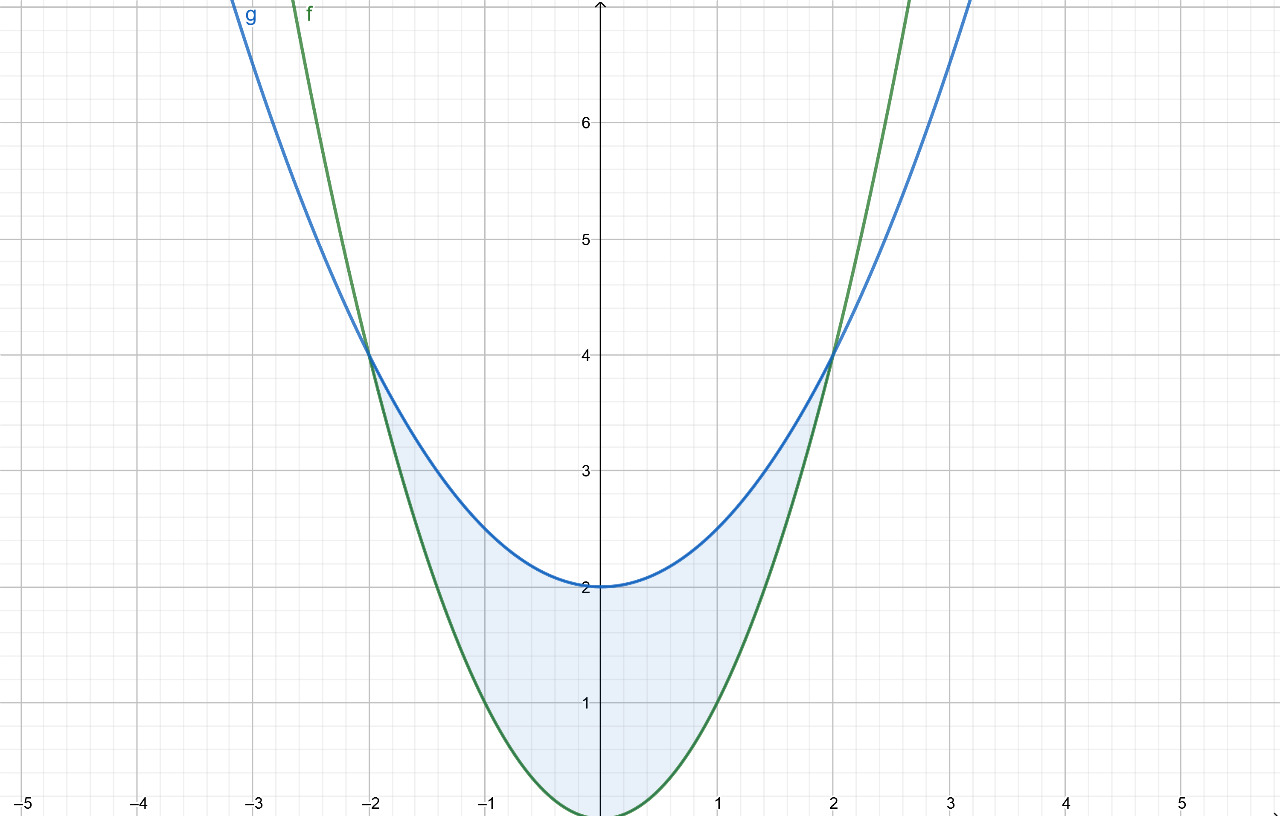
\includegraphics[width=0.5\textwidth]{7-a}
        \end{figure}
        
        Primero debemos observar donde se intersecan para entender que area esta contenida entre las funciones, \(x^2=\displaystyle\frac{x^2}{2}+2\)
        \[2x^2=x^2+4\Rightarrow x^2=4\Rightarrow x=\pm 2\]
        Las funciones se cruzan en \((-2,4)\) y \((2,4)\) y sabemos, por su imagen, que \(x^2<\displaystyle\frac{x^2}{2}+2\) en \([-2,2]\)\medskip
        El area contenida entre dos funciones puede ser representada como la diferencia entre el area de la superior y el de la inferior.\medskip

        La primitiva de \(x^n\) es \(x^{n-1}/(n-1)\) y la de \(c\) es \(cx\).
        \begin{align*}
            \int_{-2}^{2}\left(\frac{x^2}{2}+2\right)dx - \int_{-2}^{2}x^2dx&= \int_{-2}^{2}\frac{x^2}{2}dx + \int_{-2}^{2}2dx - \int_{-2}^{2}x^2dx\\
            &= \left[\frac{2^3}{6}-\frac{(-2)^3}{6}\right]+\big[2(2)-2(-2)\big]-\left[\frac{2^3}{3}-\frac{(-2)^3}{3}\right]\\
            &= \left[\frac{8}{6}+\frac{8}{6}\right]+8-\left[\frac{8}{3}+\frac{8}{3}\right]\\
            &= \frac{8}{3}+8-\frac{16}{3} = \frac{8}{3}+\frac{24}{3}-\frac{16}{3}\\
            &= \frac{16}{3}
        \end{align*}

    %EJERCICIO B
    \item Las gr\'aficas de \(f(x)=x^2\) y \(g(x)=1-x^2\).\bigskip
    
        Observemos como funciona la funcion que aun no conocemos:\bigskip

        La funcion \(1-x^2\) tiene: \medskip

        \textbf{Dominio: }\(\mathbb{R}\) ya que nunca se indetermina.\medskip

        \textbf{Imagen: }\medskip
        \begin{equation*}
            y=1-x^2 \Rightarrow x^2=1-y \Rightarrow x = \sqrt{1-y} \Rightarrow 1-y\geq0 \Rightarrow y\leq1
        \end{equation*}

        \(Img(f): [1,\infty]\)\medskip

        \textbf{Continuidad: } x no tiene restricciones y resta de continuas es continua.\medskip

        \textbf{Raices: }\(1-x^2=0\Rightarrow x^2=1\Rightarrow x=\pm1\) o \(x=\pm1\)\medskip

        \textbf{Paridad: }\(1-x^2 = 1-(-x)^2=1-x^2\) es par\medskip

        \textbf{Derivadas: }\(g'(x)=-2x \qquad g''(x)=-2\)\medskip

        \textbf{Puntos y valores criticos: }\(-2x=0\Rightarrow x=0\) y sustituyendo en \(g'(x)\Rightarrow -2(0)=0\) (No nos dice nada). Pero al evaluar en \(f(0)=1-0^2=1\), \((0,1)\), por la imagen, es un m\'aximo\medskip

        \textbf{Crecencia: }\(-2x>0\Rightarrow x<0\) Por lo que es Creciente en \(x<0\). \(-2x<0\Leftrightarrow x>0\) Por lo que es decreciente en \(x>0\)\medskip

        \textbf{Concavidad y Convexidad: } \(g''(x)<0\) es c\'oncava siempre y no tiene puntos de inflexi\'on.\medskip

        \begin{figure}[ht]
            \centering
            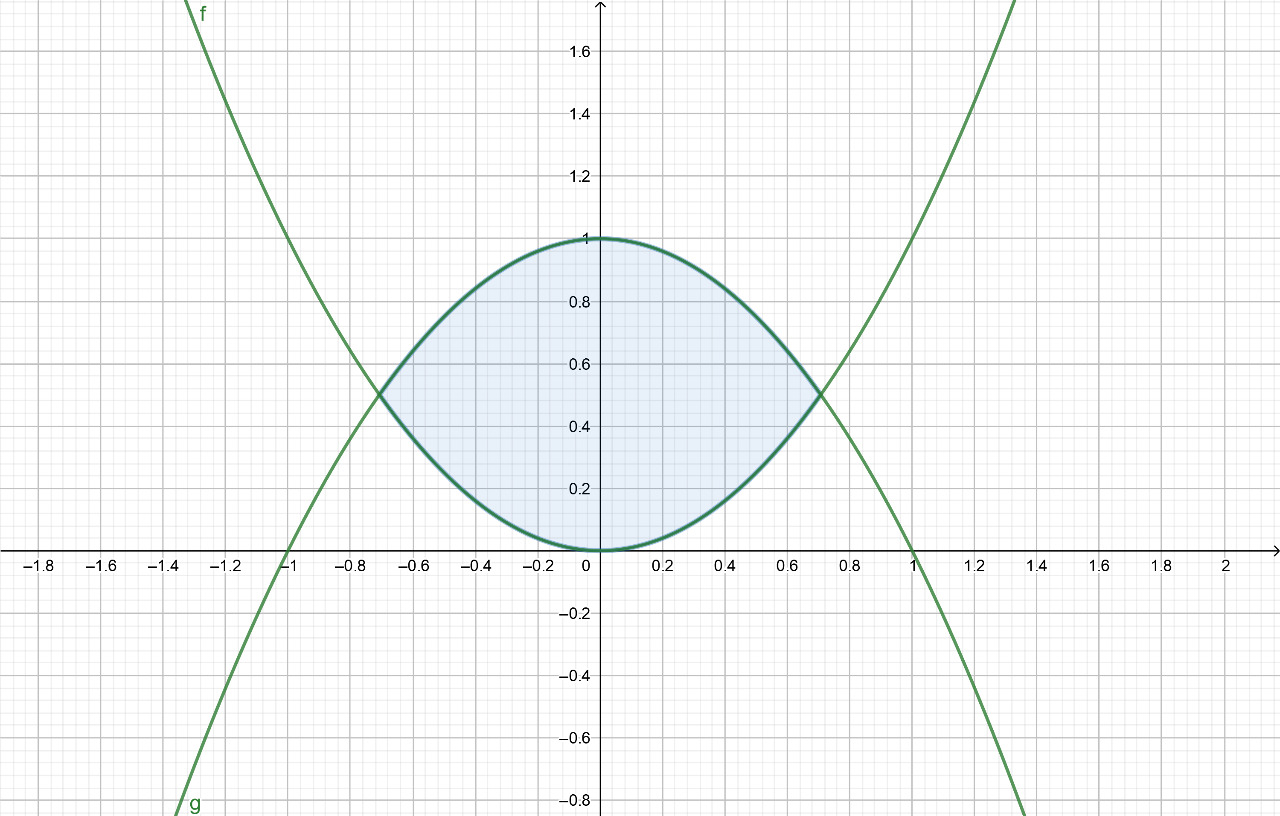
\includegraphics[width=0.5\textwidth]{7-b}
        \end{figure}

        Veamos donde se intersecan las funciones \(x^2=1-x^2\) 
        \[2x^2=1\Rightarrow x^2=\displaystyle\frac{1}{2}\Rightarrow x=\pm\displaystyle\frac{1}{\sqrt{2}}\]
        Las funciones se cruzan en \(\left(-\frac{1}{\sqrt{2}},\displaystyle\frac{1}{2}\right)\) y \(\left(\frac{1}{\sqrt{2}},\displaystyle\frac{1}{2}\right)\) y por sus derivadas y sus puntos c\'iticos podremos saber que en el intervalo \(1-x^2\) es la funcion superior.\medskip

        El area contenida entre dos funciones puede ser representada como la diferencia entre el area de la superior y el de la inferior.\medskip
        \begin{align*}
            \int_{-\frac{1}{\sqrt{2}}}^{\frac{1}{\sqrt{2}}}(1-x^2)dx - \int_{-\frac{1}{\sqrt{2}}}^{\frac{1}{\sqrt{2}}} x^2dx &= \int_{-\frac{1}{\sqrt{2}}}^{\frac{1}{\sqrt{2}}} 1dx - \int_{-\frac{1}{\sqrt{2}}}^{\frac{1}{\sqrt{2}}} x^2dx - \int_{-\frac{1}{\sqrt{2}}}^{\frac{1}{\sqrt{2}}} x^2dx\\
            &= \int_{-\frac{1}{\sqrt{2}}}^{\frac{1}{\sqrt{2}}} 1dx - 2\int_{-\frac{1}{\sqrt{2}}}^{\frac{1}{\sqrt{2}}} x^2dx\\
            &= \frac{1}{\sqrt{2}}-\left(-\frac{1}{\sqrt{2}}\right) - 2\left[\frac{\left(\frac{1}{\sqrt{2}}\right)^3}{3}-\frac{\left(-\frac{1}{\sqrt{2}}\right)^3}{3}\right]\\
            &= \frac{2}{\sqrt{2}} - 2\left[\frac{\frac{1}{2\sqrt{2}}}{3}+\frac{\frac{1}{2\sqrt{2}}}{3}\right]\\
            &= \frac{2}{\sqrt{2}} - 2\left[\frac{2}{6\sqrt{2}}\right] = \frac{2}{\sqrt{2}} - \frac{4}{6\sqrt{2}}\\
            &= \frac{12-4}{6\sqrt{2}} = \frac{8}{6\sqrt{2}} = \frac{4}{3\sqrt{2}}
        \end{align*}
        NOTA: \((\sqrt{2})^3 = (2^{1/2})^3 = 2^{3(1/2)} = 2^{3/2} = \sqrt{2^3} = \sqrt{2\cdot2^2} = 2\sqrt{2}\)\medskip

    %EJERCICIO C
    \item Las gr\'aficas de \(f(x)=x^2\) y \(g(x)=1-x^2\) y \(h(x)=2\).\medskip
    
        Observemos como se comporta la funcion que aun no conocemos\medskip

        La funcion \(h(x)=2\) tiene:\bigskip

        \textbf{Dominio: }\(\mathbb{R}\) ya que nunca se indetermina.\medskip
        
        \textbf{Imagen: } \(x=2\)\medskip

        \textbf{Continuidad: }Toda constante, es continua.\medskip

        \textbf{Raices: }\(2\neq0\) No tiene.\medskip
        
        \textbf{Paridad: }\(2=2\) Par.\medskip

        \textbf{Derivados: }\(h'(x)=0 \qquad h''(x)=0\)\medskip
        
        \textbf{Puntos y valores criticos: } Al ser constante todos sus puntos son m\'aximos y m\'inimos.\medskip
        
        \textbf{Crecencia: } Al ser constante no crece ni decrece.\medskip

        \textbf{Concavidad y Convexidad: } Al ser constante no es Concava ni Convexa.\bigskip

        \begin{figure}[ht]
            \centering
            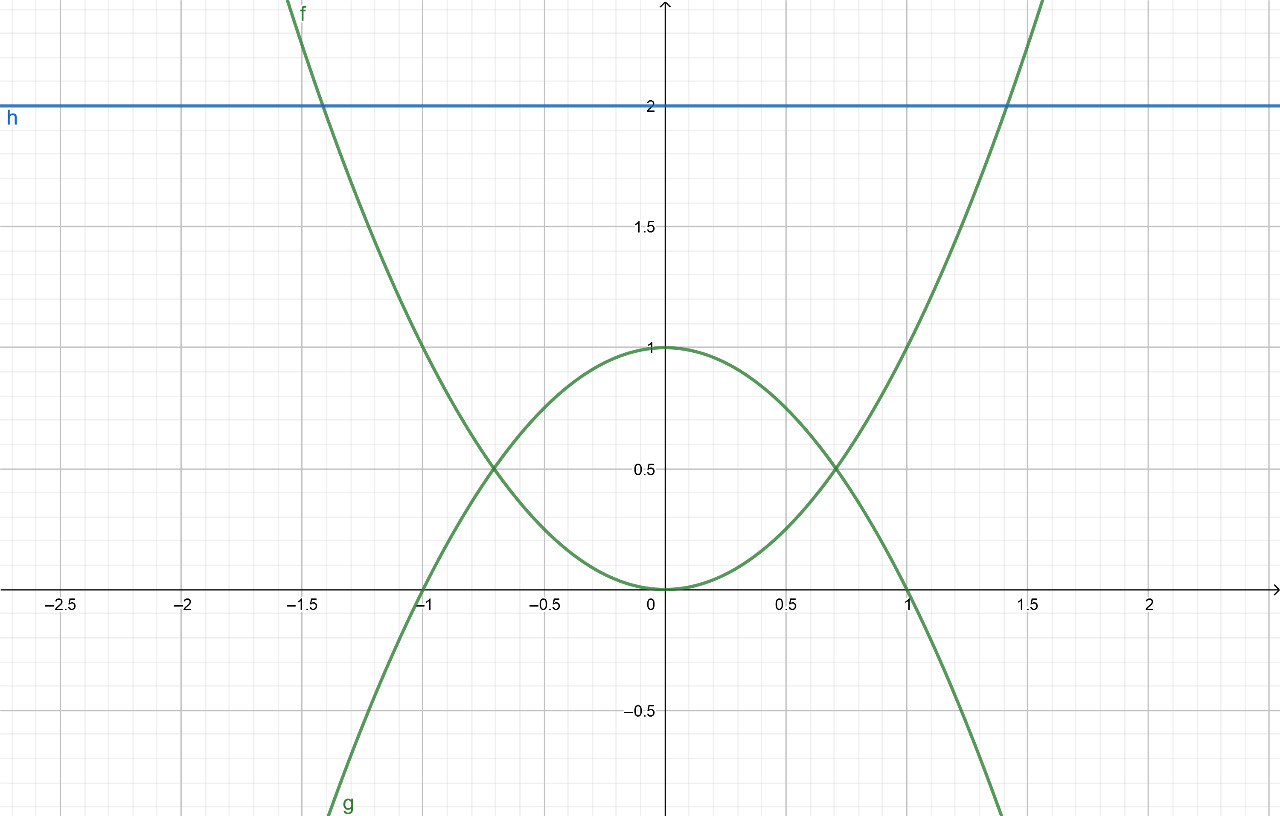
\includegraphics[width=0.5\textwidth]{7-c}
        \end{figure}

        Como ya sabemos, $f$ y $g$ se intersecan en \(\left(-\frac{1}{\sqrt{2}},\displaystyle\frac{1}{2}\right)\) y \(\left(\frac{1}{\sqrt{2}},\displaystyle\frac{1}{2}\right)\). Como \(g(x)\leq1\), nunca de encuentra con \(h\), \(f(x)\), por su par, si que se interseca con \(h\) en \((2,\sqrt{2}),\ (2,-\sqrt{2})\) (despejando x de \(2=x^2 \Rightarrow x=\pm\sqrt{2}\)).\medskip

        Seg\'un la gr\'afica tenemos que el \'area qeu buscamos est\'a denotada por: 
        \[\int_{-\sqrt{2}}^{\sqrt{2}}2dx-\int_{-\sqrt{2}}^{\sqrt{2}}x^2dx-\left[\int_{-\frac{1}{\sqrt{2}}}^{\frac{1}{\sqrt{2}}}(1-x^2)dx - \int_{-\frac{1}{\sqrt{2}}}^{\frac{1}{\sqrt{2}}} x^2dx\right]\]

        Entonces podemos usar el inciso b para decir que: 
        \[\int_{-\sqrt{2}}^{\sqrt{2}}2dx-\int_{-\sqrt{2}}^{\sqrt{2}}x^2dx-\frac{4}{3\sqrt{2}}\]
        \begin{align}
            \int_{-\sqrt{2}}^{\sqrt{2}}2dx-\int_{-\sqrt{2}}^{\sqrt{2}}x^2dx-\frac{4}{3\sqrt{2}} &= [2(\sqrt{2})-2(-\sqrt{2})] - \left[\frac{(\sqrt{2})^3}{3}-\frac{(-\sqrt{2})^3}{3}\right]-\frac{4}{3\sqrt{2}}\\
            &= 4\sqrt{2}-\left[\frac{2\sqrt{2}}{3}+\frac{2\sqrt{2}}{3}\right]-\frac{4}{3\sqrt{2}}\\
            &= 4\sqrt{2}-\frac{4\sqrt{2}}{3}-\frac{4}{3\sqrt{2}} = 4\left[\sqrt{2}-\frac{\sqrt{2}}{3}-\frac{1}{3\sqrt{2}}\right]\\
            &= 4\left[\frac{3\sqrt{2}^2-\sqrt{2}^2-1}{3\sqrt{2}}\right] = 4\left[\frac{6-2-1}{3\sqrt{2}}\right]\\
            &= 4\frac{3}{3\sqrt{2}} = \frac{4}{\sqrt{2}} = \frac{2^2}{2^{1/2}} = 2^{3/2} = 2\sqrt{2}
        \end{align}

    %EJERCICIO D
    \item Las gr\'aficas de \(f(x)=x^2\) y \(g(x)=x^2-2x+4\) y el eje vertical.\bigskip
    
        Observemos como se comporta la funcion que aun no conocemos.\medskip

        La funcion \(g(x) = x^2-2x+4\) tiene:\medskip

        \textbf{Continuidad: } Todo polinomio es continuo.\medskip

        \textbf{Dominio: }\(\mathbb{R}\) porque es un polinomio.\medskip

        \textbf{Imagen: } \(y = x^2-2x+4 \Longrightarrow x^2-2x+(4-y)=0\)\medskip

        Aplicamos la f\'ormula general con \(a=1, \ b=-2, \ c=4-y\):
        \begin{equation*}
            x=\frac{-(-2)\pm\sqrt{(-2)^2-4(1)(4-y)}}{2(1)} = \frac{2\pm\sqrt{-12+4y}}{2}
        \end{equation*}
        Entonces..
        \begin{align}
            -12+4y\geq0 \Longrightarrow 4y\geq12 \Longrightarrow y\geq3
        \end{align}
        \(Img(f): [3,\infty]\)\medskip

        \textbf{Raices: } No tiene ya que \(x\geq 3\).\medskip

        \textbf{Paridad: } \(f(-x)=(-x)^2-2(-x)+4=x^2+2x+4\) No es ni par ni impar.\medskip

        \textbf{Derivados: }\(g'(x)=2x-2 \qquad g''(x)=2\)\medskip

        \textbf{Puntos y valores criticos: } \(2x-2=0\Rightarrow 2x=2\Rightarrow x=1\) y sustituyendo en \(g(x)\Rightarrow 1^2-2\cdot1\)\((1,3)\) es un m\'inimo porque \(g''(x)>0\)\medskip

        \textbf{Crecencia: }\medskip
        
        \(2x-2<0\Rightarrow 2x<2\Leftrightarrow x<1\), $g$ es decreciente cuando \(x<1\).\medskip

        \(2x-2>0\Rightarrow 2x>2\Leftrightarrow x>1\), $g$ es creciente cuando \(x>1\).\medskip

        \textbf{Concavidad y Convexidad: }\(g''(x)>0\) Es Convexa siempre.\bigskip

        \begin{figure}[ht]
            \centering
            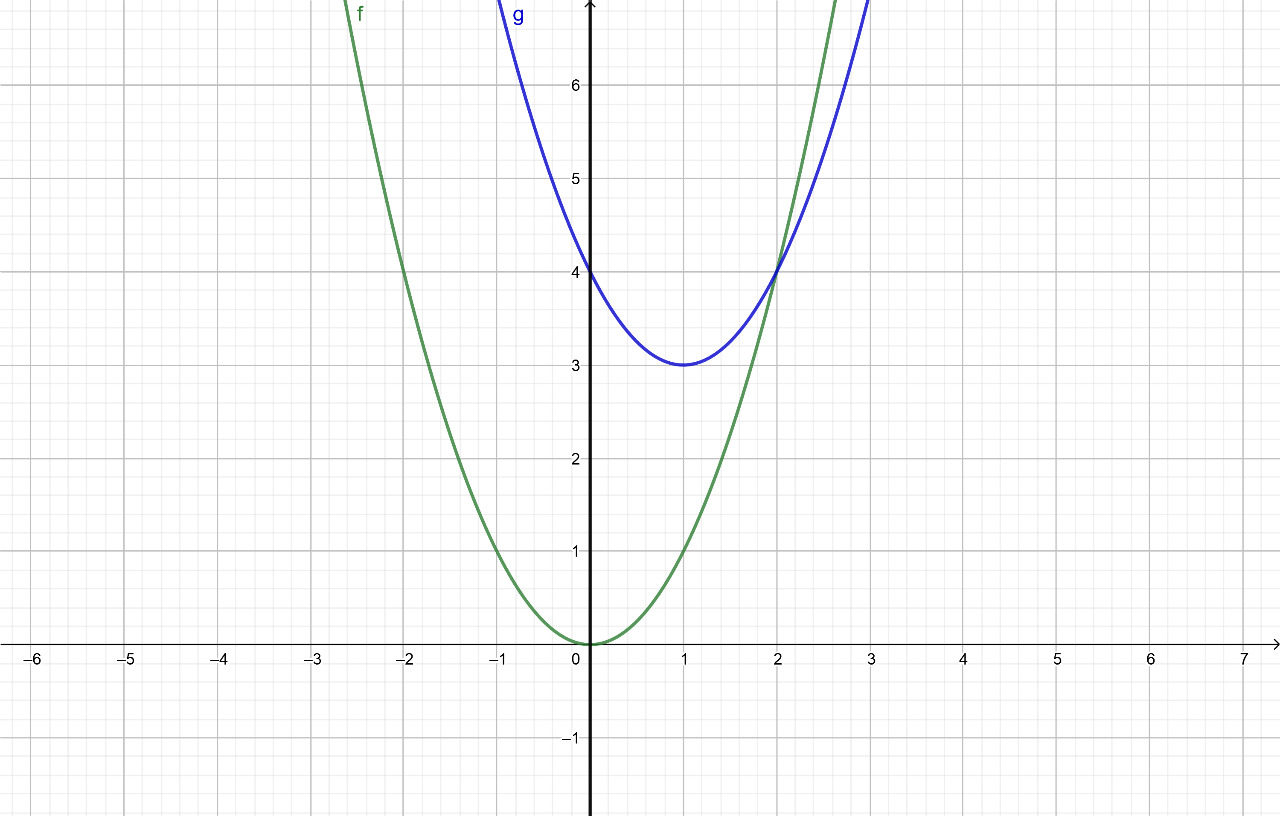
\includegraphics[width=0.5\textwidth]{7-d}
        \end{figure}

        Al usar el eje Y, tenemos uno de los extremos de nuestro rango \(x=0\), encontremos el otro \(x^2 = x^2-2x+4\Rightarrow 2x=4\Rightarrow x=2\) Asi que nuestro intervalo es \([0,2]\).\medskip

        \(0\leq x\leq2 \Longrightarrow 0\leq x^2\leq 4\) y \(0\leq2x\leq4 \Longrightarrow 0\geq -2x\geq -4 \Longrightarrow 4\geq 4-2x\geq 0\)\medskip

        Asi entonces \(x^2<x^2+(4-2x)\) (Porque \(4-2x\) es positivo en el intervalo a evaluar). entonces \(g\) es la funci\'on superior.
        \begin{align*}
            \int_{0}^{2}(x^2-2x+4)dx-\int_{0}^{2}x^2dx &= \int_{0}^{2}x^2dx -\int_{0}^{2}2xdx +\int_{0}^{2}4dx -\int_{0}^{2}x^2dx \\
            &= -2\int_{0}^{2}xdx +\int_{0}^{2}4dx = -2\left[\frac{2^2}{2}-\frac{0^2}{2}\right]+4(2)-4(0)\\
            &= -4+8=4
        \end{align*}

\end{enumerate}

%EJERCICIO 8 ----------------------------------------------------------------------------------
8. Hallar la derivada de cada una de las siguientes funciones.

\begin{enumerate}[\hspace{9px} a)]
    %EJERCICIO A
    \item \(F(x)=\displaystyle\int_{a}^{x^3}\sin^3(t)dt\)\medskip
    
        Vemos a \(F(x)\) como una composici\'on de funciones:
        \[g(x)=\int_{a}^{x}\sin^3(t)dt \qquad h(x)=x^3 \Longrightarrow F(x)=g(h(x))\]

        Derivando \(F(x)\) tenemos:
        \[F'(x)=g'(h(x))h'(x)\]
        \(h'(x)=\frac{d}{dx}x^3=3x^2\)\medskip

        \(g'(x)\): seno es continua y derivable en todos los \(\mathbb{R}\), por lo que \(\sin(x)^3\) tambi\'en lo es, adem\'as el intervalo va de \([a,x]\). As\'i podemos usar el primer teorema fundamental del c\'alculo para decir que:
        \[g'(x) = sin^3(x)\]

        Entonces: \(F'(x)=g'(h(x))h'(x) = (sin^3(x^3))(3x^2) = 3x^2\cdot\sin^3(x^3)\)\medskip
        
    %EJERCICIO B
    \item \(F(x)=\displaystyle\int_{3}^{\left(\displaystyle\int_{1}^{x}\sin^3(t)dt\right)}\frac{1}{1+\sin^6(t)+t^2}dt\)\medskip
    
        Vemos a \(F(x)\) como una composici\'on de funciones:
        \[g(x)=\int_{3}^{x}\frac{1}{1+\sin^6(t)+t^2}dt \qquad h(x)=\int_{1}^{x}\sin^3(t)dt \Longrightarrow F(x)=g(h(x))\]

        Derivando \(F(x)\) tenemos:
        \[F'(x)=g'(h(x))h'(x)\]

        Con el inciso a obtenemos \(h'(x) = \sin^3(x)\).\medskip

        \(g'(x)\): \(\sin^6(x)\geq0\) y \(t^2\geq0\) (Por ser exponentes par) \(\sin^6(x)+t^2+1>\sin^6(x)+t^2\geq0\). Por lo que el denominador nunca es 0. seno es continuo y \(t^2+1\) (polinomio) tambi\'en. As\'i \(\frac{1}{1+\sin^6(t)+t^2}\) es continua. Adem\'as el intervalo es \([3,x]\). Con lo que se puede usar el PTFC para afirmar que:
        \[g'(x) = \frac{1}{1+\sin^6(x)+x^2}\]

        Entonces: \(\displaystyle F'(x) = g'(h(x))h'(x) = \frac{\sin^3(x)}{1+\sin^6\left(\int_{1}^{x}\sin^3(t)dt\right)+\left(\int_{1}^{x}\sin^3(t)dt\right)^2}\)\medskip

    %EJERCICIO C
    \item \(F(x)=\displaystyle\int_{15}^{x}\left(\int_{8}^{y}\frac{1}{1+\sin^2(t)+t^2}dt\right)dy\)\medskip
    
        Analogo a como se demostr\'o en el inciso b, \(\displaystyle\frac{1}{1+\sin^2(t)+t^2}\) es continua. As\'i, su integral N cualquier intervalo es continua. Adem\'as el intervalo de la integral de \(F(x)\) es \([15,x]\). Por lo que se puede utilizar el PTFC para decir que:
        \[F'(x) = \int_{8}^{x}\frac{1}{1+\sin^2(t)+t^2}dt\]

\end{enumerate}

%EJERCICIO 9 ----------------------------------------------------------------------------------
9. Para cda una de las siguiente integrales impropias. Mostrar si es convergente o no seg\'un sea el caso.

\begin{enumerate}[\hspace{9px} a)]
    %EJERCICIO A
    \item \(\displaystyle\int_{0}^{\infty}x^rdx\) si $r<-1$
        \begin{equation*}
            \int_{0}^{\infty}x^rdx = \lim_{b\to\infty}\int_{0}^{b}x^rdx
        \end{equation*}

        Como la funci\'on es continua e integrable, podemos obtener una primitiva: \(g(x)=\displaystyle\frac{x^{r+1}}{r+1}\) (Como \(r<-1\) nunca de indetermina). As\'i tenemos (Por el STFC) que:
        \[\lim_{b\to\infty}\int_{0}^{b}x^rdx = \lim_{b\to\infty}\left[\frac{b^{r+1}}{r+1}-\frac{0^{r+1}}{r+1}\right] = \lim_{b\to\infty}\frac{b^{r+1}}{r+1}\]
        Como \(r<-1 \Longrightarrow r+1<0\), lo que significa que \(r+1\) siempre es negativo, por lo que \(a^{r+1}=1/a^{-(r+1)}\):
        \begin{equation*}
            \lim_{b\to\infty}\frac{b^{r+1}}{r+1} = \lim_{b\to\infty}\frac{\frac{1}{b^{-(r+1)}}}{r+1} = \frac{1}{r+1}\lim_{b\to\infty}\frac{1}{b^{-(r+1)}} \Rightarrow\ \text{Como \(-(r+1)>0\)} \Rightarrow \frac{1}{r+1}\cdot0 = 0
        \end{equation*}

        Por lo tanto, como el l\'imite existe y no es \(\pm\infty\), la integral converge.\bigskip

    %EJERCICIO B
    \item \(\displaystyle\int_{1}^{\infty}\frac{1}{x}dx\)\medskip
        
        (Resuleto en clase)\medskip

        Sabiendo que \(\displaystyle\int_1^{\displaystyle a^b}\frac{1}{x}dx = b\int_1^a\frac{1}{x}dx\). Podemos reescribir la inegral como (\(a>1\)):
        \[\int_{1}^{\infty}\frac{1}{x}dx = \lim_{b\to\infty}\int_{1}^{a^b}\frac{1}{x}dx = \lim_{b\to\infty}b\int_{1}^{a}\frac{1}{x}dx\]
        Como \(a>1\) (Por como construimos la integral), la integral es postivia, asi:
        \[\lim_{b\to\infty}b\int_{1}^{a}\frac{1}{x}dx = \int_{1}^{a}\frac{1}{x}dx\lim_{b\to\infty}b = \infty\]

        Por lo tanto, la integral diverge.\bigskip

    %EJERCICIO C
    \item \(\displaystyle\int_{0}^{a}x^rdx\) si $-1<r<0$\bigskip
        
        Analogo al ejericicio a. La primitiva es \(g(x)=\displaystyle\frac{x^{r+1}}{r+1}\):
        \begin{equation*}
            \int_{0}^{a}x^rdx = \frac{a^{r+1}}{r+1} - \frac{0^{r+1}}{r+1}
        \end{equation*}
        Como \(-1<r<0 \Rightarrow 0<r+1<1\), \(\displaystyle\frac{0^{r+1}}{r+1}=0\) por lo que:
        \begin{equation*}
            \int_{0}^{a}x^rdx = \frac{a^{r+1}}{r+1}
        \end{equation*}

        Por lo tanto, la integral converge.\bigskip

    %EJERCICIO D
    \item \(\displaystyle\int_{0}^{1}\frac{1}{x}dx\)\medskip
    
    (Resuelto en el inciso 10)\bigskip

\end{enumerate}

%EJERCICIO 10 ----------------------------------------------------------------------------------
10. Muestre que la regi\'on \(A=\{(x,y) \ | \ x<1, \ 0 \leq y \leq \frac{1}{x}\}\) tiene \'area infinita.\medskip

(Ejercicio realizado en clase).\bigskip

\textbf{Observaciones:}\medskip
\begin{itemize}
    \item $A$ se refiere al \'area bajo la curva de \(\displaystyle\frac{1}{x}\) en el intervalo $[0,1]$: \quad \(\displaystyle\int_0^1\frac{1}{x}dx\)
    \item Propiedad presentada en clase: \(\displaystyle\int_1^{\displaystyle a^b}\frac{1}{x}dx = b\int_1^a\frac{1}{x}dx\)\bigskip
\end{itemize}

Por demostrar que \(\displaystyle\int_0^1\frac{1}{x}dx = \infty\)

\begin{proof}[Prueba:]
    . \medskip

    Consideremos $b>0$ en: \(\displaystyle\lim_{b\to0}\int_b^1\frac{1}{x}dx\).\medskip

    \textbf{Nota:} \(\displaystyle\lim_{b\to\infty}\left(\frac{1}{2}\right)^b = \lim_{b\to\infty} \frac{1^b}{2^b} = \lim_{b\to\infty} \frac{1}{2^b} = 0\)\bigskip

    Entonces podemos reescribir la f\'omula como:

    \[\lim_{b\to\infty}\int_{\left(\frac{1}{2}\right)^b}^1\frac{1}{x}dx\]

    Usando las propiedades de las integales y la propiedad de las observaciones tenemos que:

    \begin{align*}
        \lim_{b\to\infty}\int_{\left(\frac{1}{2}\right)^b}^1\frac{1}{x}dx = \lim_{b\to\infty}-\int^{\left(\frac{1}{2}\right)^b}_1\frac{1}{x}dx = \lim_{b\to\infty}-b\cdot\int^{\left(\frac{1}{2}\right)}_1\frac{1}{x}dx
    \end{align*}

    \textbf{Observaci\'on:} \(\displaystyle\int^{\left(\frac{1}{2}\right)}_1\frac{1}{x}dx <0\) porque \(1/2<1\). Entonces \(\displaystyle-\int^{\left(\frac{1}{2}\right)}_1\frac{1}{x}dx >0\)\bigskip

    Por tanto:
    \[\lim_{b\to\infty}-b\cdot \int^{\left(\frac{1}{2}\right)}_1\frac{1}{x}dx  = \lim_{b\to\infty}b\cdot -\int^{\left(\frac{1}{2}\right)}_1\frac{1}{x}dx = \infty\]

    Por transitividad: \qquad \(\displaystyle\int_0^1\frac{1}{x}dx = \infty\)\medskip

\end{proof}

%EJERCICIO 11 ----------------------------------------------------------------------------------
11. Encontrar la gr\'afica de las siguientes funciones.

\begin{enumerate}[\hspace{9px} a)]
    %EJERCICIO A
    \item \(f(x)=\tan(x)-x\)\bigskip
    
        \textbf{Continuidad: }\medskip

            $x$ es un polinomio, por lo que es continua en todos los $\mathbbm{R}$, \(\tan(x)\) es continua en \(\mathbbm{R}\setminus\displaystyle\left\{\frac{(2k+1)\pi}{2}, k\in\mathbbm{Z}\right\}\) porque es donde su denominador (\(\cos(x)\)) se iguala a 0. as\'i entonces \(f(x)\) es continua en \(\mathbbm{R}\setminus\displaystyle\left\{\frac{(2k+1)\pi}{2}, k\in\mathbbm{Z}\right\}\).\bigskip
        
        \textbf{Dominio: }\medskip
            
            Dada la continuidad de la funci\'on y debido al dominio de \(tan(x)\):\medskip

            \(Dom(f):\mathbbm{R}\setminus\displaystyle\left\{\frac{(2k+1)\pi}{2}, k\in\mathbbm{Z}\right\}\)\bigskip

        \textbf{Imagen: }\medskip

            Analizamos la funci\'on en torno a $\tan(x)$ (Una func\'ion ya definida en clase), y tenemos que:

            \begin{align*}
                \tan(x)-x<\tan(x) \quad \text{si} \ x>0\\
                \tan(x)-x>\tan(x) \quad \text{si} \ x<0
            \end{align*}

            Con lo anterior y sabiendo que \(\tan(x)\) no est\'a acotada, tenemos que \(\tan(x)-x\) tampoco lo est\'a, asi: \(Img(f): \mathbbm{R}\)\bigskip

        \textbf{Ra\'ices: }\medskip
            \begin{align*}
                \tan(x)-x=0 \Rightarrow \tan(x)=x \Rightarrow \frac{\sin(x)}{\cos(x)}=x
            \end{align*}

            Un punto en el que esto sucede es cuando \(x=0\): \(\tan(0)-0=0\)

            Esto ocurre cuando $\tan(x)$ est\'a en el intervalo \((-\pi/2,\pi/2)\). CAbe recordar que como la funci\'on es siempre creciente s\'olo puede tocar una vez el 0 por periodo.

        \textbf{Paridad: }\medskip

            Partimos sabiendo que \(\sin(-x)=-\sin(x)\) (seno es impar) y que \(\cos(-x)=\cos(x)\) (coseno es par).

            \begin{align*}
                f(-x)&=\tan(-x)-(-x)=\frac{\sin(-x)}{\cos(-x)}+x \\
                &= \frac{-\sin(x)}{\cos(x)}+x = -\tan(x)+x \\
                &= -(\tan(x)-x)= -f(x)
            \end{align*}

            $f$ es impar.\bigskip

        \textbf{Derivadas: }\medskip

            Sabiendo que: \(\displaystyle\frac{d}{dx}\tan(x) = \displaystyle\frac{1}{\cos^2(x)}\)

            \begin{align*}
                f'(x) &= \frac{d}{dx}\tan(x) - \frac{d}{dx}x = \frac{1}{\cos^2(x)} - 1 = \frac{1}{\cos^2(x)} - \frac{\cos^2(x)}{\cos^2(x)} \\
                &= \frac{1-\cos^2(x)}{\cos^2(x)} = \frac{\sin^2(x)}{\cos^2(x)} = \tan^2(x)
            \end{align*}

            \begin{align*}
                f''(x) &= \frac{d}{dx}\tan^2(x)\cdot\frac{d}{dx}\tan(x) = 2\cdot\tan(x)\cdot\frac{1}{\cos^2(x)} \\
                &= 2\cdot\frac{\sin(x)}{\cos(x)}\cdot\frac{1}{\cos^2(x)} = \frac{2\sin(x)}{\cos^3(x)}
            \end{align*}
            
        \textbf{Puntos y valores cr\'iticos: }\medskip

            \begin{equation*}
                f'(x)=0 \Longrightarrow \tan^2(x)=0 \Longrightarrow \frac{\sin(x)}{\cos(x)}=0 \Longrightarrow \sin(x)=0
            \end{equation*}

            Sabemos, por la definici\'on dada en clase, que \(\sin(x)=0\) en \(x=k\pi, \ k\in\mathbbm{Z}\), as\'i entonces 
            \[f'(x)=0 \quad \text{si} \ x=k\pi, \ k\in\mathbbm{Z}\]

            Para los valores cr\'iticos tenemos que \(\tan^2(x)=0, \quad \text{si} \ x=k\pi, \ k\in\mathbbm{Z}\), asi:

            \begin{equation*}
                f(x) = \tan(x)-x \quad \text{con } \  x=k\pi, \ k\in\mathbbm{Z}
            \end{equation*}

            Como en esos puntos \(\tan(x)=0\), entonces tendremos: \[f(x)=-x \quad \text{con } \  x=k\pi, \ k\in\mathbbm{Z} \Longrightarrow (k\pi,-k\pi) \quad \text{con } \  x=k\pi, \ k\in\mathbbm{Z}\]

        \textbf{Crecencia: }\medskip

            Analizando \(f'(x)\) tenemos que \(\tan^2(x)>0 \ \forall x\in\mathbbm{R}\) (Por el cuadrado), as\'i, $f$ siempre es creciente.

        \textbf{Puntos y valores de Inflexi\'on: }\medskip

            \begin{equation*}
                f''(x)=0 \Longrightarrow \frac{2\sin(x)}{\cos^3(x)} \Longrightarrow \sin(x)=0
            \end{equation*}

            Analogo al an\'alisis de los puntos cr\'iticos (Pues en ambos casos llegamos \(\sin(x)=0\)), tendremos que los valores de inflexi\'on ser\'an:
            \[(k\pi,-k\pi) \quad \text{con } \  x=k\pi, \ k\in\mathbbm{Z}\]

            Lo que tambi\'em significa que todos nuestros puntos cr\'itcos son puntos de inflexi\'on, por lo que la funci\'on no tiene nim\'inimos ni m\'aximos.

        \textbf{Concavidad y Convexidad: }\medskip

        CONVEXIDAD:
        \begin{equation*}
            \frac{2\sin(x)}{\cos^3(x)}>0 
            \begin{cases}
                2\sin(x)>0 \wedge \cos^3(x)>0 \qquad \sin(x)>0 \wedge \cos(x)>0 \quad \dots (1)\\ \\
                2\sin(x)<0 \wedge \cos^3(x)<0 \qquad \sin(x)<0 \wedge \cos(x)<0 \quad \dots (2)
            \end{cases}
        \end{equation*}

        Analizando con \(0<x<2\pi\)

        \begin{equation*}
            (1) \dots \ \sin(x)>0 \wedge \cos(x)>0 \Longrightarrow (0,\pi) \cap ([0,\pi/2) \cup (3\pi/2,2\pi]) \Longrightarrow \left(0,\frac{\pi}{2}\right)
        \end{equation*}

        \begin{equation*}
            (2) \dots \ \sin(x)<0 \wedge \cos(x)<0 \Longrightarrow (\pi,2\pi) \cap (\pi/2,3\pi/2) \Longrightarrow \left(\pi,\frac{3\pi}{2}\right)
        \end{equation*}

        Basados en que el periodo de \(\tan(x)\) es $\pi$, extendemos el intervalo y obtenemos que $f$ es c\'convexa en:
        \[\left(k\pi,\frac{\pi}{2}+k\pi\right) \ k\in\mathbbm{Z}\]

        CONCAVIDAD:
        \begin{equation*}
            \frac{2\sin(x)}{\cos^3(x)}<0 
            \begin{cases}
                2\sin(x)>0 \wedge \cos^3(x)<0 \qquad \sin(x)>0 \wedge \cos(x)<0 \quad \dots (1)\\ \\
                2\sin(x)<0 \wedge \cos^3(x)>0 \qquad \sin(x)<0 \wedge \cos(x)>0 \quad \dots (2)
            \end{cases}
        \end{equation*}

        \begin{equation*}
            (1) \dots \ \sin(x)>0 \wedge \cos(x)<0 \Longrightarrow (0,\pi) \cap (\pi/2,3\pi/2) \Longrightarrow \left(\frac{\pi}{2},\pi\right)
        \end{equation*}

        \begin{equation*}
            (2) \dots \ \sin(x)<0 \wedge \cos(x)>0 \Longrightarrow (\pi,2\pi) \cap ([0,\pi/2) \cup (3\pi/2,2\pi]) \Longrightarrow \left(\frac{3\pi}{2},2\pi\right)
        \end{equation*}

        Al igual que con la convexidad usamos la propiedad periodica de $\tan(x)$ para extender el intervalo:
        \[\left(\frac{\pi}{2}+k\pi,k\pi+\pi\right) \ k\in\mathbbm{Z}\]

        \textbf{Gr\'afica: }\medskip

        \begin{figure}[ht]
            \centering
            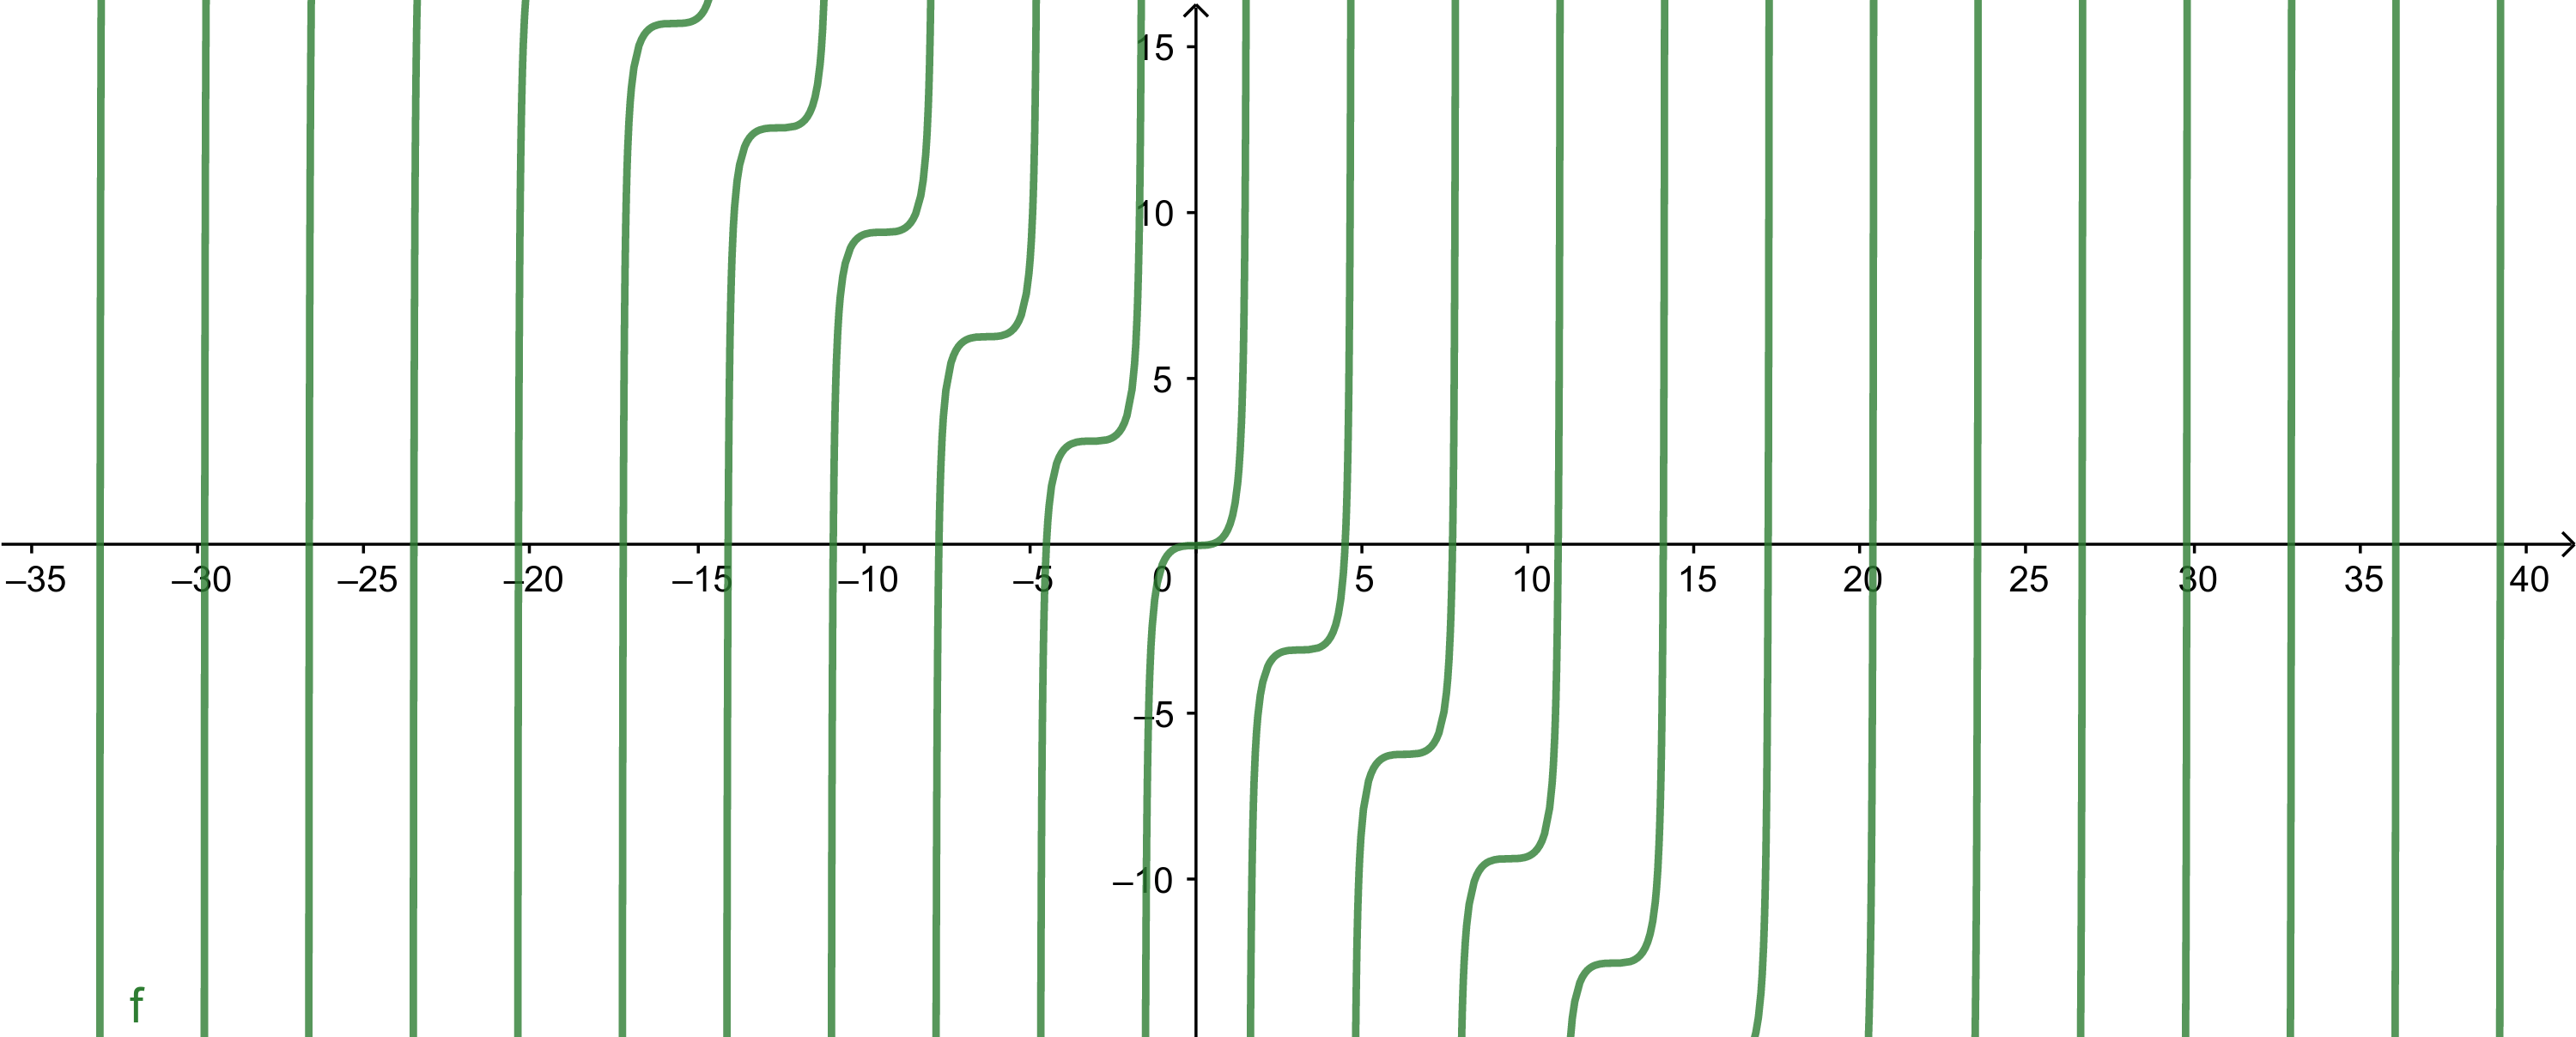
\includegraphics[width=0.5\textwidth]{11-a}
        \end{figure}

    %EJERCICIO B
    \item \(f(x)=x+\sin(x)\)\bigskip
    
    \textbf{Continuidad: }\medskip

        $x$ es una recta continua y \(sin(x)\) es tambi\'en continuo en todos los $\mathbbm{R}$. Por lo que \(f(x)\) es continua en todos los $\mathbbm{R}$.\medskip

    \textbf{Dominio: }\medskip

        Como no hay nig\'un punto en el que la funci\'on est\'e indefinida: \(Dom(f): \mathbbm{R}\)\medskip

    \textbf{Imagen: }\medskip
        \begin{equation*}
            -1\leq\sin(x)\leq1 \Longrightarrow x-1\leq x+\sin(x)\leq x+1
        \end{equation*}

        Lo que significa que \(f(x)\) est\'a por debajo de \(x+1\) (y \(x+1\) no est\'a acotada inferiormente) y por encima de \(x-1\) (y \(x-1\) no est\'a acotada superiormente). \(x+\sin(x)\) no est\'a acotada, por lo que: \(Img(f): \mathbbm{R}\)\medskip

    \textbf{Ra\'ices: }\medskip

        \(x+1\) tiene ra\'iz en -1 (\((-1)+1=0\)) y \(x-1\) tiene ra\'iz en 1 \(1-1=0\). Como \(f(x)\) est\'a entre dichas funciones, s\'olo puede tener ra\'iz en \([-1,1]\), buscando la \(x\in[-1,1]\) tal que \(f(x)=0\), encontramos que el \'unico punto posible es \(x=0 \Rightarrow f(0)=0-\sin(0)=0-0=0\) (Cosa que se respalda dado que la funci\'on es impar).\medskip

    \textbf{Paridad: }\medskip

        Sabiendo que \(\sin(-x)=-\sin(x)\) (seno es impar):
        \begin{align*}
            f(-x)=(-x)+\sin(-x)=-x-\sin(x)=-(x+\sin(x))=-f(x) \quad \text{(es impar)}
        \end{align*}

    \textbf{Derivadas: }
        \begin{align*}
            f'(x) = \frac{d}{dx}[x+\sin(x)] = 1+\cos(x)
        \end{align*}

        \begin{align*}
            f''(x) = \frac{d}{dx}[1+\cos(x)]=-\sin(x)        
        \end{align*}

    \textbf{Puntos y valores cr\'iticos: }
        \begin{align*}
            f'(x)=0 \Longrightarrow 1+\cos(x)=0 \Longrightarrow \cos(x)=-1
        \end{align*}

        Sabemos que \(\cos(x)=-1\) en \([0,2\pi]\) s\'olo cuando \(x=\pi\) (Por la definici\'on geom\'etrica de coseno) y su que s periodo es \(2\pi\), por lo que los puntos cr\'iticos de $f$ son:
        \[x=(2k+1)\pi, \ k\in\mathbbm{Z}\]

        Evaluando \(f(\pi)=\pi+\sin(\pi)=\pi+0=\pi\) y otro pnto cr\'itico: \(f(-\pi)=-\pi+\sin(-\pi)=-\pi+0=-\pi\)\medskip

        Por lo que los valores cr\'iticos de \(f\) son (considerando el periodo de seno (\(2\pi\))):
        \[([2k+1]\pi,[2k+1]\pi), \ k\in\mathbbm{Z}\]

    \textbf{Crecencia: }
        \begin{align*}
            -1\leq\cos(x)\leq1 \Longrightarrow 1-1\leq1+\cos(x)\leq1+1 \Longrightarrow 0\leq1+\cos(x)\leq2 
        \end{align*}

        Habiendo acotado \(f'(x)=x+\cos(x)\) nos damos cuenta de que \(f'(x)>0\) en todos los puntos en los que no es 0 (Los puntos cr\'iticos), por lo que la funci\'on es siempre creciente.\medskip

    \textbf{Puntos y valores de Inflexi\'on: }
        \begin{equation*}
            f''(x)=0 \Longrightarrow -\sin(x)=0 \Longrightarrow \sin(x)=0 
        \end{equation*}

        Sabemos, por la definici\'on de seno, que \(\sin(x)=0\) cuando \(x=\pi \ \vee x=0 \vee x=2\pi\), lo que, aplicando el periodo de \(\sin(x)\), se reescribe como:
        \[x=k\pi, k\in\mathbbm{Z} \quad \text{(Puntos de inflexión)}\]

        Valores de inflexi\'on:
        \[f(k\pi)=k\pi+\sin(k\pi)=k\pi+0=k\pi \Longrightarrow (k\pi,k\pi), k\in\mathbbm{Z}\]

    \textbf{Concavidad y Convexidad: }\medskip
    
        CONCAVIDAD:
        \begin{equation*}
            f''(x)>0 \Longrightarrow -\sin(x)>0 \Longrightarrow \sin(x)<0
        \end{equation*}

        Sabemos, por definici\'on, que \(\sin(x)<0\) en \((\pi,2\pi)\), que aplicando el periodo de \(\sin(x)\) nos proporciona los intervalos:
        \[(2k\pi+\pi, \ 2k\pi+2\pi), k\in\mathbbm{Z}\]

        CONVEXIDAD:
        \begin{equation*}
            f''(x)<0 \Longrightarrow -\sin(x)<0 \Longrightarrow \sin(x)>0
        \end{equation*}

        Sabemos, por definici\'on, que \(\sin(x)>0\) en \((0,\pi)\), que aplicando el periodo de \(\sin(x)\) nos proporciona los intervalos:
        \[(2k\pi, \ 2k\pi+\pi), k\in\mathbbm{Z}\]

    \textbf{Gr\'afica: }\medskip

    \begin{figure}[ht]
        \centering
        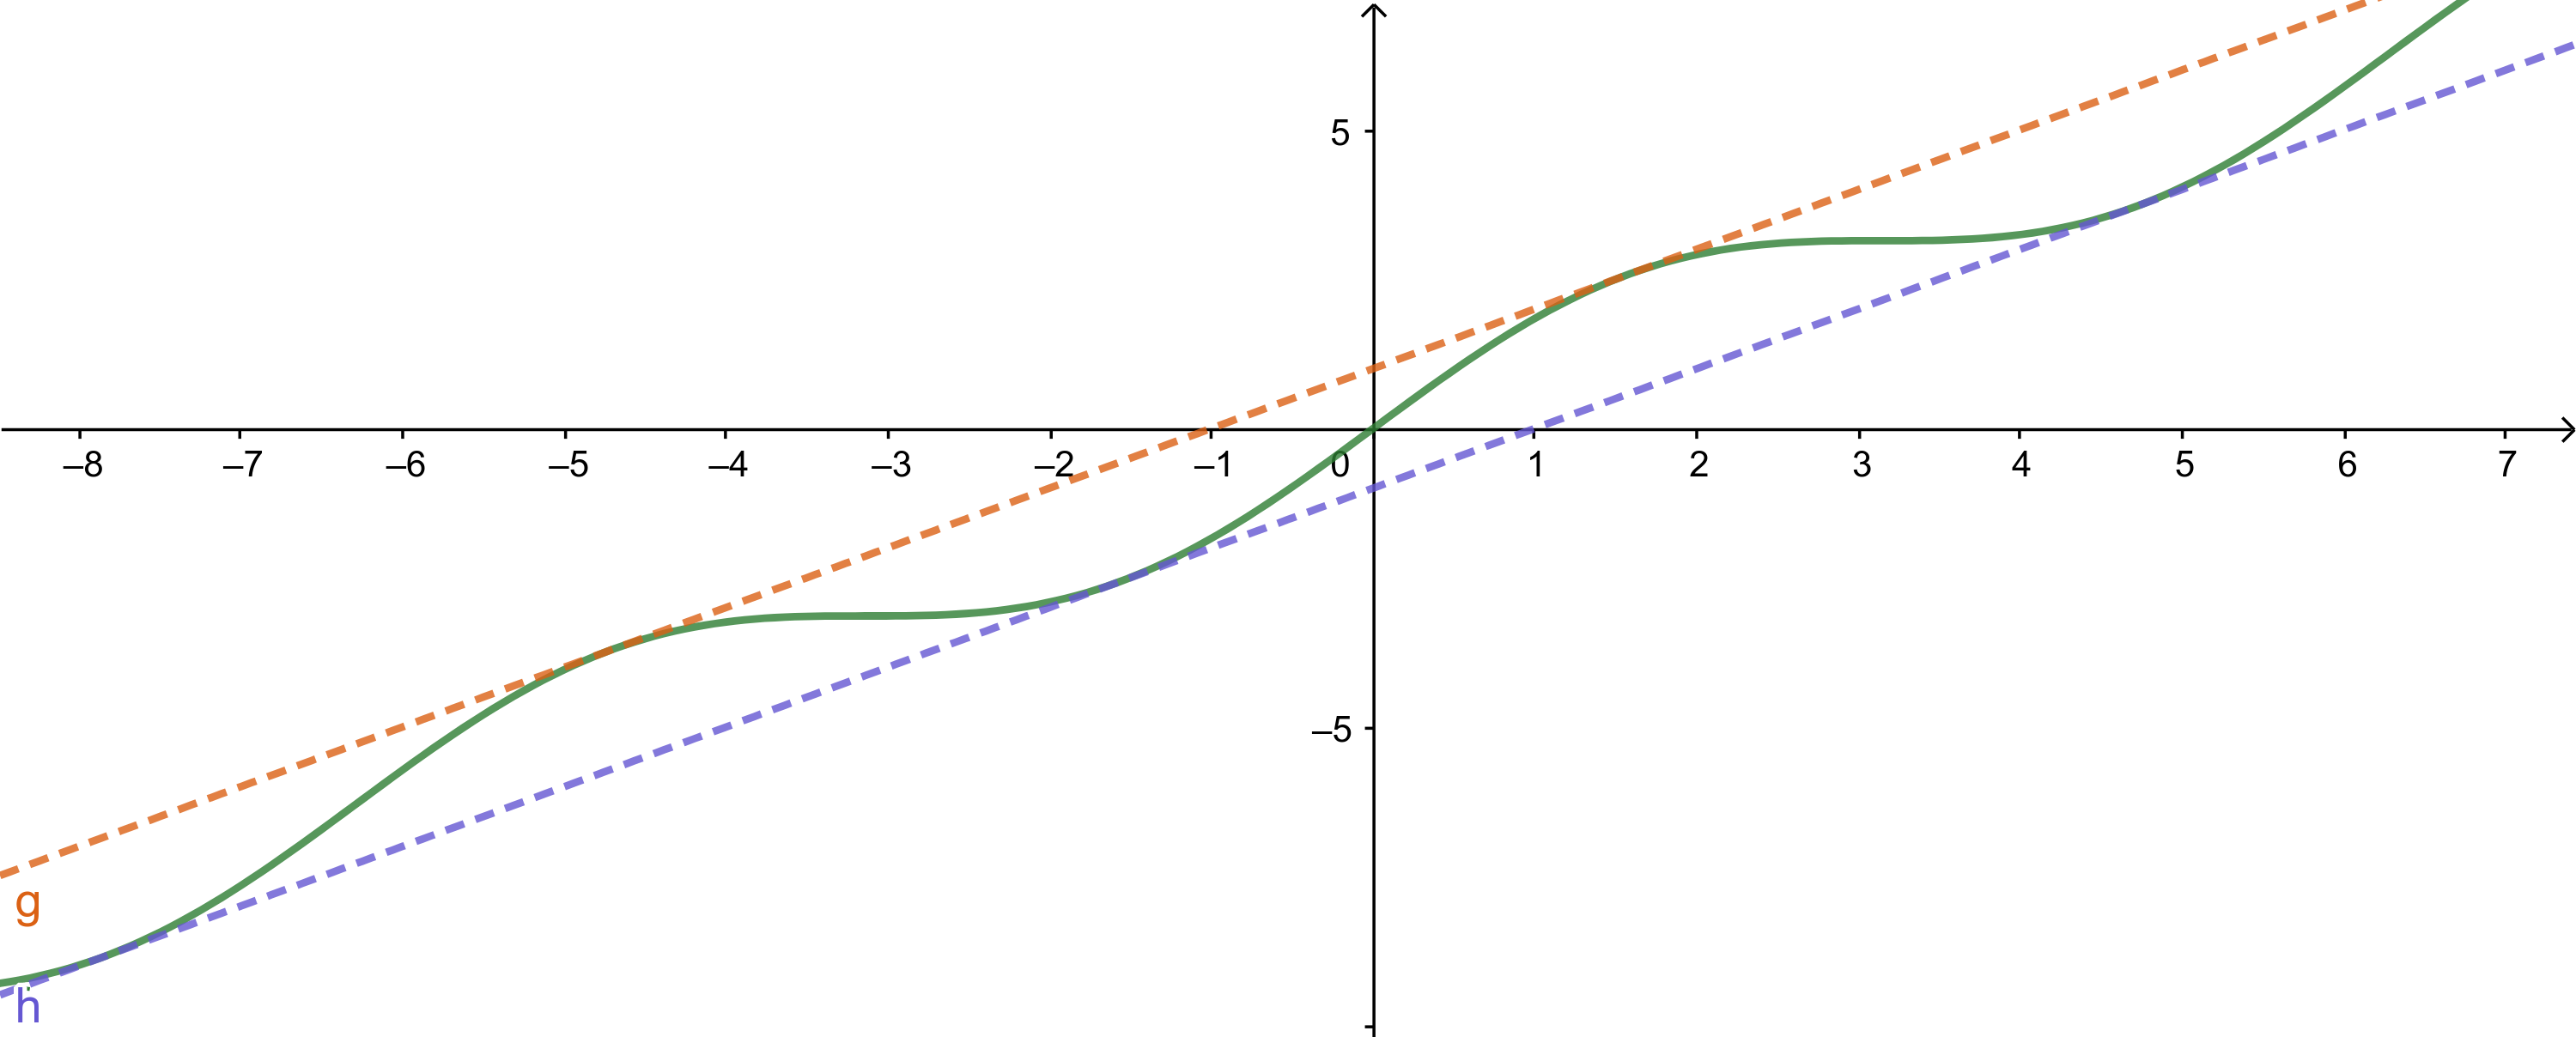
\includegraphics[width=0.5\textwidth]{11-b}
    \end{figure}

    %EJERCICIO C
    \item \(f(x)=\sin(x)+\sin(2x)\)\bigskip
    
    \textbf{Continuidad: }\medskip

        \(\sin(x)\) y \(\sin(2x)\) son funciones continuas en todos los \(\mathbbm{R}\), por lo que su suma (\(\sin(x)+\sin(2x)\)), tambi\'en es continua en todos los \(\mathbbm{R}\).\medskip

    \textbf{Dominio: }\medskip

        Como no hay nug\'un punto en el que la funci\'on no est\'e definida: \(Dom(f): \mathbbm{R}\)\medskip

    \textbf{Imagen: }
        \begin{equation*}
            -1\leq<sin(2x)\leq1 \quad \text{y} \quad -1\leq\sin(x)\leq1
        \end{equation*}

        Asi que:
        \begin{equation*}
            -1-1<\sin(x)+\sin(2x)<1+1 \Longrightarrow -2<\sin(x)+\sin(2x)<2
        \end{equation*}

        La imagen que obtenemos es: \(I:[-2,2]\). Pero resulta no ser exacta, ps \(\sin(x_0)\) no es igual que \(\sin(x_0)\). Por lo que resulta es un desface en la suma de las funciones, por lo que, en realidad, la imagen de $f$ es un subconunto de I.\medskip

    \textbf{Ra\'ices: }
        \begin{equation*}
            \sin(x)+\sin(2x) = \sin(x)+2\sin(x)\cos(x) = \sin(x)(1+2\cos(x))
        \end{equation*}

        As\'i entonces, \(f(x)=0\) cuando \(\sin(x)=0 \Longrightarrow x=2k\pi, k\in\mathbbm{Z}\) y cuando \(1+2\cos(x)=0\)\medskip

        Sabemos que \(f(\pi/2)=1+2\cos(\pi/2)=1+0=1\) y que \(f(\pi) = 1+2\cos(\pi) = 1-2 = -1\), por lo que, por el TVI (Porque la funci\'on es continua), sabemos que hay una ra\'iz en \((\pi/2,\pi)\)\medskip

        Usando el m\'etodo de Newton-Raphson:
        \begin{equation*}
            x_1 = x_0 - \frac{f(x_0)}{f'(x_0)} = \frac{\pi}{2} - \frac{\sin(\frac{\pi}{2})+\sin(2\frac{\pi}{2})}{\cos(\frac{\pi}{2})+2\cos(2\frac{\pi}{2})} = \frac{\pi}{2}+\frac{1+0}{0+2(-1)} = \frac{\pi}{2}-\frac{1}{2}
        \end{equation*}

        Resulta ser una buena aproximaci\'on a la ra\'iz que, probando numeros, queda \(f(2\pi/3) = 0\) y \(\displaystyle\frac{2\pi}{3}\approx\frac{\pi}{2}-\frac{1}{2}\) (No la usaremos en la descripci\'on pues se obtuvo con calculos no permitidos).\medskip

        As\'i, las raices de \(f\) son:
        \begin{align*}
            x = 2k\pi \quad \text{y} \quad x = \frac{2k\pi}{3}, \ k\in \mathbbm{Z}
        \end{align*}

    \textbf{Paridad: }\medskip
        
        Sabiendo que \(\sin(x)\) es par:
        \begin{equation*}
            f(-x)=\sin(-x)+\sin(-2x) = -\sin(x) - \sin(2x) = -(\sin(x)+\sin(2x)) = -f(x)
        \end{equation*}

    \textbf{Derivadas: }
        \begin{align*}
            f'(x) &= \frac{d}{dx}[\sin(x)+\sin(2x)] = \cos(x) + 2\cos(2x) \\
            &= \cos(x) + 2(\cos^2(x)-\sin^2(x)) = \cos(x) + 2(\cos^2(x)-(1-\cos^2(x))) \\
            &= \cos(x) + 2(2\cos^2(x)-1) = 4\cos^2(x)+\cos(x)-2
        \end{align*}

        \begin{align*}
            f''(x) = \frac{d}{dx}[\cos(x) + 2\cos(2x)] = -\sin(x) - 2\cdot2\sin(2x) = -\sin(x) - 4\sin(2x)
        \end{align*}

    \textbf{Puntos y valores cr\'iticos: }
        \begin{align*}
            f'(x) = 0 \Longrightarrow 4\cos^2(x)+\cos(x)-2=0
        \end{align*}

        Sustituendo con \(u=\cos(x)\) tenemos que:
        \begin{equation*}
            4u^2+u-2=0 \quad \text{a=4, b=1, c=-2}
        \end{equation*}
        \begin{equation*}
            \cos(x) = u = \frac{-1\pm\sqrt{1^2-4(4(-2))}}{2(4)} = \frac{-1\pm\sqrt{33}}{8}
        \end{equation*}
        Acotando lo obtenido tenemos dos casos:
        \begin{align*}
            (1) \quad &25<33<36 \Longrightarrow \sqrt{25}<\sqrt{33}<\sqrt{36} \Longrightarrow 5<\sqrt{33}<6 \\
            &\Longrightarrow 4<-1+\sqrt{33}<5 \\
            &\Longrightarrow 0<\frac{1}{2}<\frac{-1+\sqrt{33}}{8}<\frac{5}{8}<1
        \end{align*}
        \begin{align*}
            (2) \quad &25<33<36 \Longrightarrow \sqrt{25}<\sqrt{33}<\sqrt{36} \Longrightarrow -5>-\sqrt{33}>-6 \\
            &\Longrightarrow -6>-1-\sqrt{33}>-7 \\
            &\Longrightarrow 0>-\frac{3}{4}>\frac{-1-\sqrt{33}}{8}>-\frac{7}{8}>-1
        \end{align*}

        Entonces los puntos cr\'iticos en \([-1,1]\): \medskip
        
        \(\cos(x_0)=\displaystyle\frac{-1+\sqrt{33}}{8} \Longrightarrow x = \arccos\left(\frac{-1+\sqrt{33}}{8}\right)\) y \medskip
        
        \(\cos(x_1)=\displaystyle\frac{-1-\sqrt{33}}{8} \Longrightarrow x = \arccos\left(\frac{1+\sqrt{33}}{8}\right)\)

        Donde \(\arccos(0)<x_0<\arccos(1) \Longrightarrow \frac{3\pi}{2}<x_0<2\pi\) y \(\arccos(-1)<x_1<\arccos(0) \Longrightarrow \frac{\pi}{2}<x_0<\pi\).

        Al extender ambos puntos por el periodo tendremos:
        \begin{align*}
            x_0 = \pm\arccos\left(\frac{-1+\sqrt{33}}{8}\right)+2k\pi \ , \ x_1 = \pm\arccos\left(\frac{1+\sqrt{33}}{8}\right)+2k\pi+\pi\ , \ k\in\mathbbm{R}
        \end{align*}
        NOTA: El \(\pm\) se debe a que \(\cos(-x)=\cos(x)\)\medskip

        Como la derivada de \(\cos(x)\) es \(-\sin(x)\) y \(\frac{3\pi}{2}<x_0<2\pi\). En dicho intervalo \(\sin(x)<0\), por lo que el punto que observamos es un m\'aximo cuando tomamos el positivo y un m\'inimo cuando tomamos el negativo (porque lo tomamos del cuadrante contrario, sonde seno (por se impar) es poitivo).

        Analogo es el caso de \(\frac{\pi}{2}<x_0<\pi\). Intervalo donde \(\sin(x)<0\). Por lo que si tomamos el positivo el punto es in m\'aximo y si tomamos el negativo un m\'inimo

        Analizamos la funci\'on en base a los puntos cr\'iticos obtenidos con respecto a \(\cos(x)\) y a \(\sin(x)\) para obtener los datos restantes.

    \textbf{Gr\'afica: }\medskip

    \begin{figure}[ht]
        \centering
        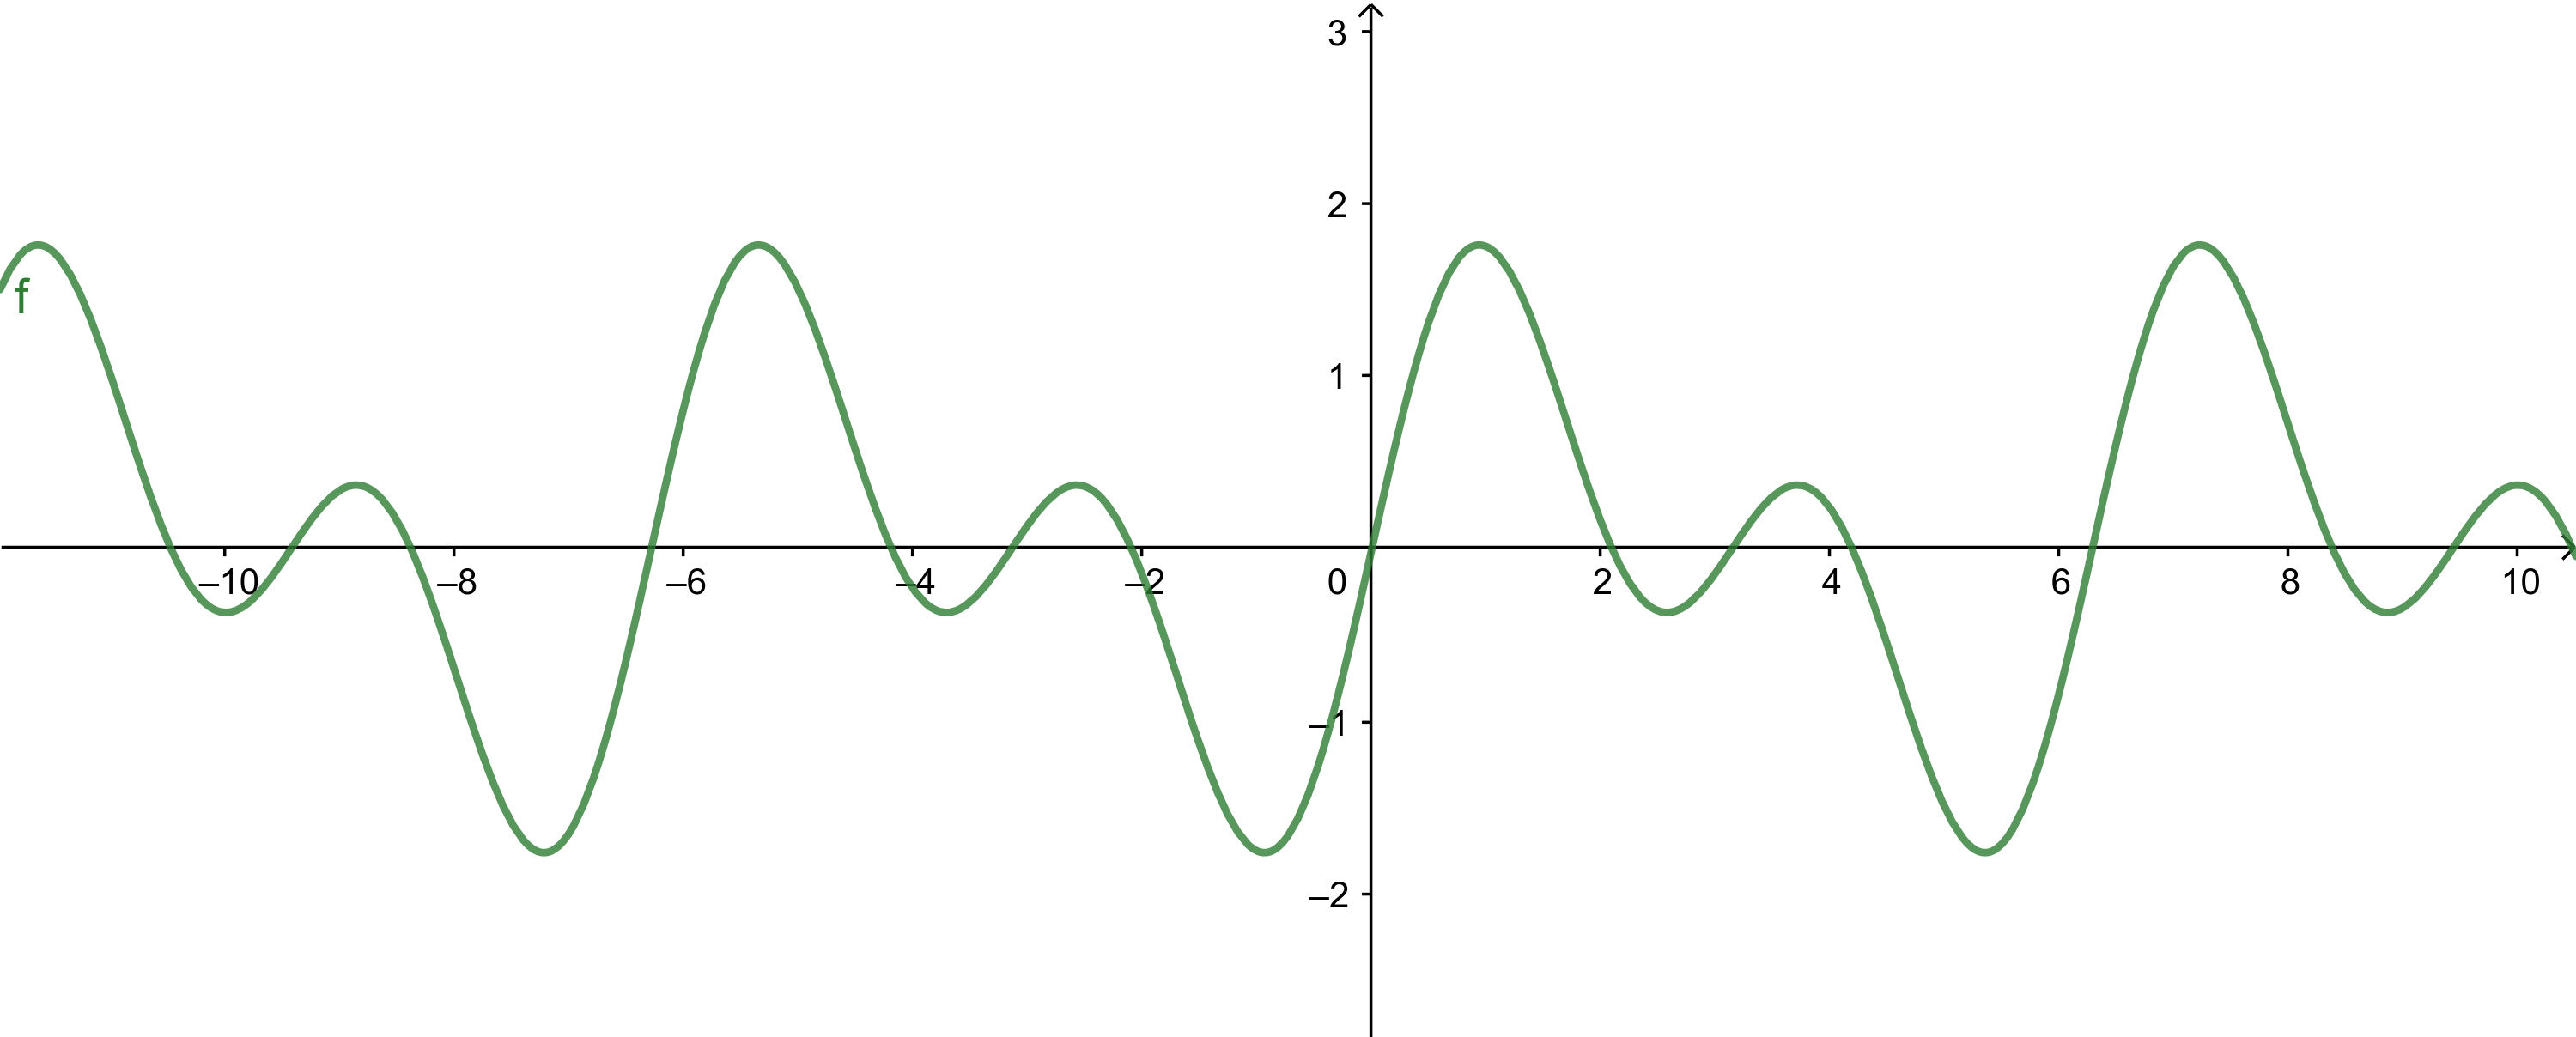
\includegraphics[width=0.5\textwidth]{11-c}
    \end{figure}

\end{enumerate}

%EJERCICIO 12 ----------------------------------------------------------------------------------
12.
\begin{enumerate}[\hspace{9px} a)]
    %EJERCICIO A
    \item Partiendo de la f\'ormula para $\cos(2x)$, deducir las f\'ormulas para $\sin^2(x)$ y $\cos^2(x)$ en t\'erminos de $\cos(2x)$.\bigskip
    
        Sabemos que: \(\cos(2x)=\cos(x+x)=\cos^2(x)-\sin^2(x)\).\bigskip
        %COS
        Desarrollando lo anterior para tener a $\cos(x)$ en t\'erminos de $\cos(2x)$:
        \begin{align*}
            \cos(2x) &= \cos^2(x)-\sin^2(x) = \cos^2(x)-\sin^2(x) + 0 \\
            &= \cos^2(x)-\sin^2(x) + \cos^2(x) - \cos^2(x) \\
            &= \cos^2(x) + \cos^2(x) -(\sin^2(x)+\cos^2(x)) = 2\cos^2(x)-1
        \end{align*}
        \begin{equation*}
            \cos(2x)= 2\cos^2(x)-1 \Longrightarrow \cos^2(x) = \frac{1+\cos(2x)}{2}
        \end{equation*}
        %SIN
        Ahora para $\sin(x)$:
        \begin{align*}
            \cos(2x) &= \cos^2(x)-\sin^2(x) = \cos^2(x)-\sin^2(x) + 0 \\
            &= \cos^2(x)-\sin^2(x) + \sin^2(x) - \sin^2(x) \\
            &= \cos^2(x)+\sin^2(x) - \sin^2(x) - \sin^2(x) = 1 - 2\sin^2(x)
        \end{align*}
        \begin{equation*}
            \cos(2x) = 1 - 2\sin^2(x) \Longrightarrow \sin^2(x) = \frac{1-\cos(2x)}{2}
        \end{equation*}

    %EJERCICIO B
    \item Mostrar que \(\cos\left(\displaystyle\frac{x}{2}\right)=\sqrt{\frac{1+\cos(x)}{2}}\) y \(\sin\left(\displaystyle\frac{x}{2}\right)=\sqrt{\frac{1-\cos(x)}{2}}\) para \(0 \leq x \leq \displaystyle\frac{\pi}{2}\).\bigskip
        %COS
        Por el inciso anterior sabemos que: \(\cos^2(x) = \displaystyle\frac{1+\cos(2x)}{2}\)\bigskip

        Proponemos un cambio de variable tal que \(t=2x\), con lo que tenemos:
        \[\cos^2(x) = \frac{1+\cos(2x)}{2} \Longrightarrow \cos^2\left(\displaystyle\frac{t}{2}\right)=\frac{1+\cos(t)}{2}\]

        Como, por hip\'otesis, \(0 \leq t \leq \displaystyle\frac{\pi}{2}\), \(0\leq\displaystyle\frac{t}{2}<\frac{\pi}{4}\). Por lo que \(1\geq\cos(t)\geq0\) y \(\displaystyle\frac{1+\cos(2t)}{2}>0\) por lo que podemos sacar ra\'iz cuadrada a ambos lados, asi:
        \[\cos\left(\displaystyle\frac{t}{2}\right)=\sqrt{\frac{1+\cos(t)}{2}}\]

        NOTA: Aunque la ra\'z denota un $\pm$, como ya especificamos que, dado el intervalo, $\cos(x)$ es mayor a 0, podemos dar por especificado el signo positivo. El caso ser\'a el mismo para $\sin(x)$.\bigskip

        %SIN
        Ahora con seno: \(\sin^2(x) = \frac{1-\cos(2x)}{2}\)\bigskip

        Proponemos un cambio de variable tal que \(t=2x\), con lo que tenemos:
        \[\sin^2(x) = \frac{1-\cos(2x)}{2} \Longrightarrow \sin^2\left(\displaystyle\frac{t}{2}\right)=\frac{1-\cos(t)}{2}\]

        Como, por hip\'otesis, \(0 \leq t \leq \displaystyle\frac{\pi}{2}\), \(0\leq\displaystyle\frac{t}{2}<\frac{\pi}{4}\). Por lo que \(0\leq\sin(t)\leq1\) y \(\frac{1-\cos(2t)}{2}>0\) (por que \(1=\cos(0)\leq\cos(2t)\leq\cos(\pi)=-1 \Longrightarrow 1-\cos(2t)>0\) por lo que podemos sacar ra\'iz cuadrada a ambos lados, asi:
        \[\sin\left(\displaystyle\frac{t}{2}\right)=\sqrt{\frac{1-\cos(t)}{2}}\]

    %EJERCICIO C
    \item Usar el primer inciso para calcular \(\displaystyle\int_{a}^{b}\sin^2(x)dx\) y \(\displaystyle\int_{a}^{b}\cos^2(x)dx\).
    
        \textbf{NOTA:} Obtenemos \(\displaystyle\int_{a}^{b}\cos(2x)dx\):\medskip

        Buscamos una primitiva cuya derivada sea $\cos(2x)$. Sabemos que \(\displaystyle\frac{d}{dx}\sin(x)=\cos(x)\), y, por ende, que \(\displaystyle\frac{d}{dx}\sin(2x)=\frac{d}{dx}\sin(2x)\cdot \frac{d}{dx}2x = 2\cos(2x)\). Como ese dos no figura en la integral, dividimos entre dos la primitiva al inicio: \(\displaystyle\frac{d}{dx}\sin(2x)/2=\frac{1}{2}\cdot\frac{d}{dx}\sin(2x)\cdot \frac{d}{dx}2x = \frac{2\cos(2x)}{2} = \cos(2x)\).\bigskip

        Asi: \quad \(\displaystyle\int_{a}^{b}\cos(2x)dx = \frac{\sin(2x)}{2}+c\).\bigskip

        \textbf{Observaciones:}
        \begin{itemize}
            \item \(\sin^2(x) = \displaystyle\frac{1-\cos(2x)}{2}\)
            \item \(\cos^2(x) = \displaystyle\frac{1+\cos(2x)}{2}\)
            \item \(\sin^2(x)+\cos^2(x)=1\)
            \item \(\sin(2x) = \sin(x+x)=2\sin(x)\cos(x)\)
            \item \(\cos(2x) = \cos^2(x)-\sin^2(x)\)
        \end{itemize}
        %SIN
        \begin{align*}
            \int_{a}^{b}\sin^2(x)dx& = \int_{a}^{b}\frac{1-\cos(2x)}{2}dx = \frac{1}{2}\int_{a}^{b}(1-\cos(2x))dx \\
            &= \frac{1}{2}\left[\int_{a}^{b}1dx - \int_{a}^{b}\cos(2x)dx\right] = \frac{1}{2}\left[x - \frac{\sin(2x)}{2}\right] \\
            &=\frac{x}{2} - \frac{\sin(2x)}{4} = \frac{2x-\sin(2x)}{4} \\
            &= \frac{2x-2\sin(x)\cos(x)}{4} = \frac{2(x-\sin(x)\cos(x))}{4} \\
            &= \frac{x-\sin(x)\cos(x)}{2}
        \end{align*}
        %COS
        \begin{align*}
            \int_{a}^{b}\cos^2(x)dx& = \int_{a}^{b}\frac{1+\cos(2x)}{2}dx = \frac{1}{2}\int_{a}^{b}(1+\cos(2x))dx \\
            &= \frac{1}{2}\left[\int_{a}^{b}1dx + \int_{a}^{b}\cos(2x)dx\right] = \frac{1}{2}\left[x + \frac{\sin(2x)}{2}\right] \\
            &=\frac{x}{2} + \frac{\sin(2x)}{4} = \frac{2x+\sin(2x)}{4} \\
            &= \frac{2x+2\sin(x)\cos(x)}{4} = \frac{2(x+\sin(x)\cos(x))}{4} \\
            &= \frac{x+\sin(x)\cos(x)}{2}
        \end{align*}

\end{enumerate}

%EJERCICIO 13 ----------------------------------------------------------------------------------
13. Mostrar que:

\begin{enumerate}[\hspace{9px} a)]
    %EJERCICIO A
    \item \(\arcsin'(x)=\displaystyle\frac{1}{\sqrt{1-x^2}}\), si \(-1<x<1\) \bigskip
    
        \textbf{Observaciones:}
        \begin{itemize}
            \item \(\displaystyle\frac{d}{dx}\big(h^{-1}(x)\big) = \frac{1}{h'(h^{-1})}\)
            \item \(\sin'(x) = \cos'(x)\)
            \item \(\sin^2(x)+\cos^2(x)=1\)
            \item \(\sin(\arcsin(x))=x \Longrightarrow \sin^2(\arcsin(x))=x^2\)
        \end{itemize}

        \begin{proof}[Prueba:]
            . \medskip

            Considerando que $\arcsin$ es la inversa de $\sin$ tenemos que su derivada esta denotada por la f\'ormula anterior (Aplicando las observaciones):
            \[\arcsin'(x) = \frac{1}{\sin'(\arcsin(x))} = \frac{1}{\cos(\arcsin(x))}\]

            Despejando \(\cos(x)\) de \(\sin^2(x)+\cos^2(x)=1\), tenemos que: \(\cos(x) = \sqrt{1-\sin^2(x)}\). Sustituyendo lo obtenido en la ecuaci\'on:

            \[\frac{1}{\cos(\arcsin(x))} = \frac{1}{\sqrt{1-\sin^2(\arcsin(x))}} = \frac{1}{\sqrt{1-x^2}}\]

            Finalmente, por transitividad:
            \[\arcsin'(x) = \frac{1}{\sqrt{1-x^2}}\]
        \end{proof}

    %EJERCICIO B
    \item \(\arccos'(x)=\displaystyle-\frac{1}{\sqrt{1-x^2}}\), si \(-1<x<1\) \bigskip
    
        \textbf{Observaciones:}
        \begin{itemize}
            \item \(\displaystyle\frac{d}{dx}\big(h^{-1}(x)\big) = \frac{1}{h'(h^{-1})}\)
            \item \(\cos'(x) = -\sin'(x)\)
            \item \(\sin^2(x)+\cos^2(x)=1\)
            \item \(\cos(\arccos(x))=x \Longrightarrow \cos^2(\arccos(x))=x^2\)
        \end{itemize}

        \begin{proof}[Prueba:]
            . \medskip

            Considerando que $\arccos$ es la inversa de $\cos$ tenemos que su derivada esta denotada por la f\'ormula anterior (Aplicando las observaciones):
            \[\arccos'(x) = \frac{1}{\cos'(\arccos(x))} = \frac{1}{-\sin(\arccos(x))}\]

            Despejando \(\sin(x)\) de \(\sin^2(x)+\cos^2(x)=1\), tenemos que: \(\sin(x) = \sqrt{1-\cos^2(x)}\). Sustituyendo lo obtenido en la ecuaci\'on:

            \[-\frac{1}{\sin(\arccos(x))} = -\frac{1}{\sqrt{1-\cos^2(\arcsin(x))}} = -\frac{1}{\sqrt{1-x^2}}\]

            Finalmente, por transitividad:
            \[\arccos'(x) = -\frac{1}{\sqrt{1-x^2}}\]
        \end{proof}

    %EJERCICIO C
    \item \(\arctan'(x)=\displaystyle\frac{1}{1+x^2}\), para toda $x$. \bigskip
        
        \textbf{Observaciones:}
        \begin{itemize}
            \item \(\displaystyle\frac{d}{dx}\big(h^{-1}(x)\big) = \frac{1}{h'(h^{-1})}\)
            \item \(\tan'(x) = \sec^2(x)\)
            \item \(\sec^2(x)=1+\tan^2(x)\)
            \item \(\tan(\arctan(x))=x \Longrightarrow \tan^2(\arctan(x))=x^2\)
        \end{itemize}

        \begin{proof}[Prueba:]
            . \medskip

            Considerando que $\arctan$ es la inversa de $\tan$ tenemos que su derivada esta denotada por la f\'ormula anterior (Aplicando las observaciones):
            \[\arctan'(x) = \frac{1}{\tan'(\arctan(x))} = \frac{1}{\sec^2(\arctan(x))} = \frac{1}{1+\tan^2(\arctan(x))} = \frac{1}{1+x^2}\]

            Por transitividad:
            \[\arctan'(x) = \frac{1}{1+x^2}\]
        \end{proof}

\end{enumerate}

%EJERCICIO 14 ----------------------------------------------------------------------------------
14. Aplicar la derivaci\'on logar\'itmica para obtener la derivada $f'(x)$ de cada una de las siguientes funciones:

\begin{enumerate}[\hspace{9px} a)]
    %EJERCICIO A
    \item \(f(x)=(1+x)(1+e^{x^2})\)\bigskip
    
        Aplicamos logaritmo natural a ambos lados de la igualdad:
        \[\ln(f(x))=\ln((1+x)(1+e^{x^2}))\]

        Por las propiedades del \(\ln\) tenemos: \quad \(\ln(f(x))=\ln(1+x)+\ln(1+e^{x^2})\)

        Derivando:
        \begin{align*}
            \frac{d}{dx}\ln(f(x)) &= \frac{d}{dx}(\ln(1+x)+\ln(1+e^{x^2}))\\
            \frac{f'(x)}{f(x)} &= \frac{\frac{d}{dx}(1+x)}{1+x}+\frac{\frac{d}{dx}(1+e^{x^2})}{1+e^{x^2}} = \frac{1}{1+x}+\frac{2xe^{x^2}}{1+e^{x^2}}\\
            &= \frac{(1+e^{x^2})+(2xe^{x^2})(1+x)}{(1+x)(1+e^{x^2})}\\
            &= \frac{1+e^{x^2}+2xe^{x^2}+2x^2e^{x^2}}{(1+x)(1+e^{x^2})}\\
            f'(x)&= (1+x)(1+e^{x^2})\left[\frac{1+e^{x^2}+2xe^{x^2}+2x^2e^{x^2}}{(1+x)(1+e^{x^2})}\right]\\
            &= 1+e^{x^2}+2xe^{x^2}+2x^2e^{x^2}
        \end{align*}

    %EJERCICIO B
    \item \(f(x)=(\cos(x))^{\sin(x)}+(\sin(x))^{\cos(x)}\)\bigskip
    
        Sabiendo que \(e^{\ln(a)}=a\), lo aplicamos a cada operando de la suma: 
        \[f(x)=e^{\ln(\cos(x)^{\sin(x)})}+e^{\ln(\sin(x)^{\cos(x)})}\]

        Usando la propiedad logar\'itmica de los exponene tenemos:
        \[f(x)=e^{\sin(x)\ln(\cos(x))}+e^{\cos(x)\ln(\sin(x))}\]

        Derivando:
        \begin{align*}
            f'(x) &= \frac{d}{dx}\left[e^{\sin(x)\ln(\cos(x))}+e^{\cos(x)\ln(\sin(x))}\right] = \frac{d}{dx}\left(e^{\sin(x)\ln(\cos(x))}\right) + \frac{d}{dx}\left(e^{\cos(x)\ln(\sin(x))}\right)\\
            &= \left[e^{\sin(x)\ln(\cos(x))}\cdot \frac{d}{dx}[\sin(x)\ln(\cos(x))]\right] + \left[e^{\cos(x)\ln(\sin(x))}\cdot \frac{d}{dx}[\cos(x)\ln(\sin(x))]\right]
        \end{align*}

        Desarrolando las derivadas:
        \begin{align*}
            \frac{d}{dx}[\sin(x)\ln(\cos(x))] &= \frac{d}{dx}\sin(x)\cdot\ln(\cos(x)) + \sin(x)\cdot\frac{d}{dx}(\ln(\cos(x)))\\
            &= \cos(x)\cdot\ln(\cos(x)) + \sin(x)\cdot\frac{-\sin(x)}{\cos(x)}\\
            &=  \cos(x)\cdot\ln(\cos(x)) - \frac{\sin(x)^2}{\cos(x)}
        \end{align*}

        \begin{align*}
            \frac{d}{dx}[\cos(x)\ln(\sin(x))] &= \frac{d}{dx}\cos(x)\cdot\ln(\sin(x)) + \cos(x)\cdot\frac{d}{dx}(\ln(\sin(x)))\\
            &= -\sin(x)\cdot\ln(\sin(x))+\cos(x)\cdot\frac{\cos(x)}{\sin(x)}\\
            &= -\sin(x)\cdot\ln(\sin(x))+\frac{\cos^2(x)}{\sin(x)}
        \end{align*}

        Recordando que \(e^{\ln(a)}=a\), resustitumos todo:
        \begin{align*}
            f'(x) &= \cos(x)^{\sin(x)}\left[\cos(x)\cdot\ln(\cos(x)) - \frac{\sin(x)^2}{\cos(x)}\right]+\\
            & \quad  \ \sin(x)^{\cos(x)}\left[-\sin(x)\cdot\ln(\sin(x))+\frac{\cos^2(x)}{\sin(x)}\right]\\
            &= \left[\cos(x)^{\sin(x)}\cdot\cos(x)\cdot\ln(\cos(x)) - \cos(x)^{\sin(x)}\cdot\frac{\sin(x)^2}{\cos(x)}\right]+\\
            & \quad \ \left[-\sin(x)^{\cos(x)}\cdot\sin(x)\cdot\ln(\sin(x)) + \sin(x)^{\cos(x)}\cdot\frac{\cos^2(x)}{\sin(x)}\right]
        \end{align*}

        \begin{multline*}
            f'(x) = \cos(x)^{\sin(x)+1}\cdot\ln(\cos(x)) - \cos(x)^{\sin(x)-1}\sin^2(x) \\- \sin(x)^{\cos(x)+1}\cdot\ln(\sin(x)) + \sin(x)^{\cos(x)-1}\cos^2(x)
        \end{multline*}

    %EJERCICIO C
    \item \(f(x)=\displaystyle\frac{(3-x)^{1/3}x^3}{(1-x)(3+x)^{2/3}}\)\bigskip
        \begin{align*}
            f(x)&= \frac{(3-x)^{1/3}x^3}{(1-x)(3+x)^{2/3}} \Longrightarrow \ln(f(x)) = \ln\left(\frac{(3-x)^{1/3}x^3}{(1-x)(3+x)^{2/3}}\right)\\
            \ln(f(x)) &= \ln((3-x)^{1/3}) + \ln(x^3) - (\ln(1-x) + \ln((3+x)^{2/3}))\\
            &= \frac{1}{3}\cdot\ln(3-x) + 3\ln(x) - \ln(1-x) - \frac{2}{3}\cdot\ln(3+x)\\
            \ln(f(x))' &= \frac{d}{dx}\left[\frac{1}{3}\cdot\ln(3-x) + 3\ln(x) - \ln(1-x) - \frac{2}{3}\cdot\ln(3+x)\right]\\
            \frac{f'(x)}{f(x)} &= \frac{-1}{3(3-x)} + \frac{3}{x} - \frac{-1}{1-x} - \frac{2}{3(3+x)}\\
            f'(x)&=f(x)\left[\frac{-1}{3(3-x)} + \frac{3}{x} - \frac{-1}{1-x} - \frac{2}{3(3+x)}\right]\\
            &= \frac{(3-x)^{1/3}x^3}{(1-x)(3+x)^{2/3}}\left[\frac{-1}{3(3-x)} + \frac{3}{x} - \frac{-1}{1-x} - \frac{2}{3(3+x)}\right]\\
            f'(x)&= \frac{(3-x)^{1/3}x^3}{(1-x)(3+x)^{2/3}}\left[-\frac{1}{9-3x} + \frac{3}{x} + \frac{1}{1-x} - \frac{2}{9+3x}\right]
        \end{align*}

    %EJERCICIO D
    \item \(f(x)=\displaystyle\frac{e^x-e^{-x}}{e^{3x}(1+x^3)}\)\bigskip
        \begin{align*}
            f(x)&=\frac{e^x-e^{-x}}{e^{3x}(1+x^3)} \Longrightarrow \ln(f(x)) = \ln\left(\frac{e^x-e^{-x}}{e^{3x}(1+x^3)}\right)\\
            \ln(f(x))&= \ln(e^x-e^{-x}) - [\ln(e^{3x}) + \ln(1+x^3)]\\
            \ln(f(x))' &= \frac{d}{dx}\left[\ln(e^x-e^{-x}) - \ln(e^{3x}) - \ln(1+x^3)\right]\\
            \frac{f'(x)}{f(x)} &= \frac{\frac{d}{dx}(e^x-e^{-x})}{e^x-e^{-x}} - \frac{\frac{d}{dx}e^{3x}}{e^{3x}} - \frac{3x^2}{1+x^3}\\
            &= \frac{e^x+e^{-x}}{e^x-e^{-x}} - \frac{3e^{3x}}{e^{3x}} - \frac{3x^2}{1+x^3}\\
            &= \frac{e^x+e^{-x}}{e^x-e^{-x}} - \frac{3x^2}{1+x^3} -3\\
            f'(x) &= f(x)\left[\frac{e^x+e^{-x}}{e^x-e^{-x}} - \frac{3x^2}{1+x^3} -3\right]\\
            &= \frac{e^x-e^{-x}}{e^{3x}(1+x^3)}\left[\frac{e^x+e^{-x}}{e^x-e^{-x}} - \frac{3x^2}{1+x^3} -3\right]\\
            &= \frac{e^x-e^{-x}}{e^{3x}(1+x^3)}\cdot\frac{e^x+e^{-x}}{e^x-e^{-x}} -\frac{e^x-e^{-x}}{e^{3x}(1+x^3)}\cdot\frac{3x^2}{1+x^3} -\frac{3(e^x-e^{-x})}{e^{3x}(1+x^3)}\\
            &= \frac{e^x+e^{-x}}{e^{3x}(1+x^3)} - \frac{3x^2(e^x-e^{-x})}{e^{3x}(1+x^3)^2} - \frac{3(e^x-e^{-x})}{e^{3x}(1+x^3)}\\
            &= \frac{(1+x^3)(e^x+e^{-x})-3x^2(e^x-e^{-x})-3(e^x-e^{-x})(1+x^3)}{e^{3x}(1+x^3)^2}\\
            f'(x) &= \frac{(1+x^3)(e^x+e^{-x})-3(e^x-e^{-x})(x^3+x^2+1)}{e^{3x}(1+x^3)^2}\\
        \end{align*}

\end{enumerate}

%EJERCICIO 15 ----------------------------------------------------------------------------------
15. Hallar la gr\'afica de las siguientes funciones.

\begin{enumerate}[\hspace{9px} a)]
    %EJERCICIO A
    \item \(f(x)=e^{1+x}\)\bigskip
    
        \textbf{Continuidad: }\medskip

            \(1+x\) es un polimonio, por lo que es continuo en todos los \(\mathbbm{R}\). $e^x$ es una funci\'on continua tambi\'en, y la composici\'on de dos funciones continuas es continua, por lo que \(e^{1+x}\) es continua en todos los \(\mathbbm{R}\)

        \textbf{Dominio: }\medskip

            Por el punto anteior y por el hecho de que $x$ no tiene ning\'un tipo de restricci\'on: \(Dom(f): \mathbbm{R}\)\medskip

            NOTA: Dos puntos \'utiles para graficar la funci\'on son: \(f(0)=e^{1+0}=e\), y \(f(-1)=e^{1-1}=e^0=1\)\medskip

        \textbf{Imagen: }
            \begin{equation}
                \label{cotainfa}
                1+x>x \Longrightarrow e^{1+x}>e^x>0
            \end{equation}

            Sabiendo que: \(\lim_{x\to-\infty}e^x=0\)
            \begin{equation}
                \label{lima}
                \lim_{x\to-\infty}e^{1+x}=\lim_{x\to-\infty}e\cdot e^x=e\lim_{x\to-\infty}e^x=e\cdot(0)=0
            \end{equation}

            Por la ecuaci\'on \eqref{lima} y por la definici\'on de la exponencial, sabemos que $f(x)>0$. Luego, por la ecuaci\'on \eqref{cotainfa}, sabemos que \(e^{1+x}\) est\'a por encima de \(e^x\), sabemos tambi\'en que \(e^x\) no est\'a acotada superiormente, por lo que \(e^{1+x}\) tampoco lo est\'a. As\'i entonces, la imagen de $f$ es:
            \[Img(f): \mathbbm{R}^+\]

        \textbf{Paridad: }
            \begin{equation*}
                f(-x) = e^{1+(-x)} = e^{1-x} \qquad \text{(No es ni par ni impar)}
            \end{equation*}

        \textbf{Derivadas: }

            \begin{align*}
                f'(x) &= \frac{d}{dx}e^{1+x} = \frac{d}{dx}e^{1+x}\cdot\frac{d}{dx}(1+x) = e^{1+x}(1) = e^{1+x}
            \end{align*}

            Por lo anterior \(f''(x) = e^{1+x}\)\medskip

        \textbf{Puntos y valores cr\'iticos: }\medskip

            Como \(f'(x)=f(x)\) y ya demostramos en la imagen de la funci\'on que \'esta nunca toca el 0, asi pues, la funci\'on no tiene puntos cr\'iticos.\medskip

        \textbf{Crecencia: }\medskip

            De nuevo, como \(f'(x)=f(x)\) y \(f(x)>0 \ \forall x\in\mathbbm{R}\), la funci\'on es siempre creciente.\medskip

        \textbf{Puntos y valores de Inflexi\'on: }\medskip

            Analogo a los puntos cr\'ticos (\(f''(x)=f(x)\)), la funci\'on no tiene puntos de inflexi\'on porque \(f''(x)\) nunca es 0.\medskip

        \textbf{Concavidad y Convexidad: }\medskip

            Como \(f''(x)=f(x)\) y \(f(x)>0 \ \forall x\in\mathbbm{R}\), la funci\'on es siempre convexa.\medskip

        \textbf{Gr\'afica: }\medskip

        \begin{figure}[ht]
            \centering
            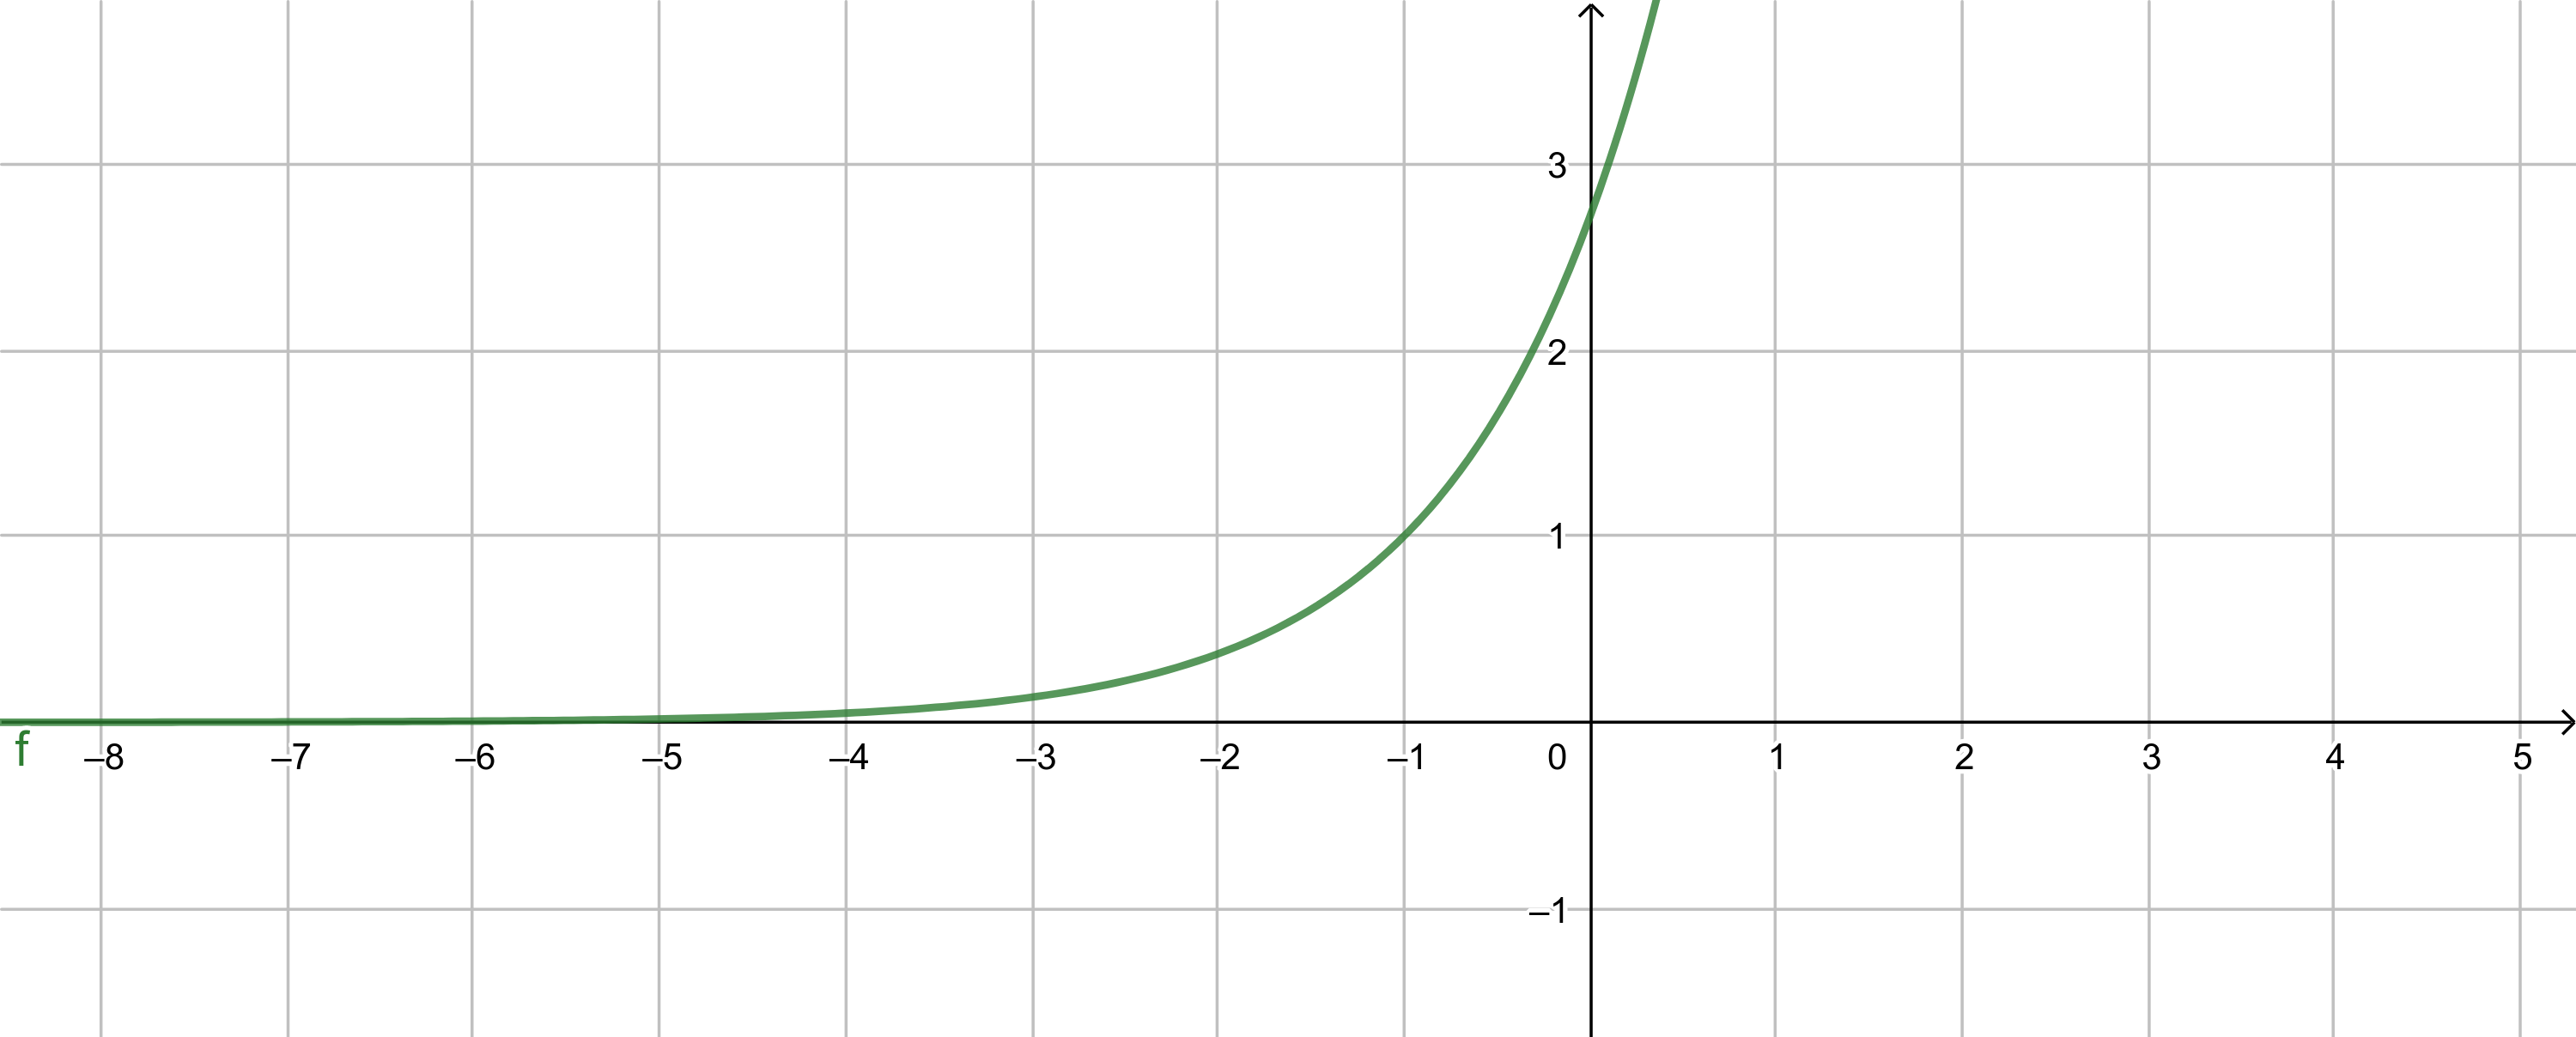
\includegraphics[width=0.5\textwidth]{15-a}
        \end{figure}

    %EJERCICIO B
    \item \(f(x)=e^{\sin(x)}\)\medskip
    
        \textbf{Continuidad: }\medskip

            \(\sin(x)\) y \(e^x\) son continuas en todos los \(\mathbbm{R}\), por lo que su compocisi\'on (\(e^{\sin(x)}\)), es continua en todos los reales.\medskip

        \textbf{Dominio: }\medskip

            Como no hay nig\'un punto en el que la funci\'on est\'e indefinida: \(Dom(f): \mathbbm{R}\)\medskip

        \textbf{Imagen: }
            \begin{equation*}
                -1\leq\sin(x)\leq1 \Longrightarrow e^{-1}\leq e^{\sin(x)}\leq e^1 \Longrightarrow Img(f):\left[\frac{1}{e},e\right]
            \end{equation*}

        \textbf{Ra\'ices: }\medskip

            Como \(\frac{1}{e}>0\), $f(x)$ nunca es 0. Por lo que \(f\) no tiene ra\'ices.\medskip

        \textbf{Paridad: }\medskip

            Sabiendo que seno es par \(\sin(-x)=\sin(x)\)
            \begin{equation*}
                f(-x) = e^{\sin(-x)} = e^{\sin(x)} = f(x) \quad \text{(es par)}
            \end{equation*}

        \textbf{Derivadas: }
            \begin{equation*}
                f'(x) = \frac{d}{dx}e^{\sin(x)}\cdot \frac{d}{dx}\sin(x) = e^{\sin(x)}\cdot\cos(x)
            \end{equation*}

            \begin{align*}
                f''(x) &= \frac{d}{dx}\left(e^{\sin(x)}\cdot\cos(x)\right) = \frac{d}{dx}e^{\sin(x)}\cdot\frac{d}{dx}\sin(x)\cdot\cos(x)+e^{\sin(x)}\cdot\frac{d}{dx}\cos(x)\\
                &= e^{\sin(x)}\cdot\cos^2(x)-e^{\sin(x)}\cdot\sin(x)\\
                &= e^{\sin(x)}\big(\cos^2(x)-\sin(x)\big)
            \end{align*}

        \textbf{Puntos y valores cr\'iticos: }
            \begin{equation*}
                f'(x)=0 \Rightarrow e^{\sin(x)}\cdot\cos(x)=0
            \end{equation*}

            Como sabemos que \(e^{\sin(x)}> \ \forall x\in\mathbbm{R}\), \(f'(x)\) s\'olo ser\'a 0 cuando \(\cos(x)=0\) que sabemos, por la definici\'on de coseno dada en clase, que eso sucede en: \(\displaystyle x=\frac{(2k+1)\pi}{2},k\in\mathbbm{Z}\)\medskip

            Sabemos tambi\'en que \(\cos(\pi/2)=0 \ \wedge \ \sin(\pi/2)=1 \Rightarrow e^{\sin(\pi/2)}=e\) y que \(\cos(3\pi/2)=0 \ \wedge \ \sin(3\pi/2)=-1 \Rightarrow e^{\sin(3\pi/2)}=e^-1\)\medskip

            Comparamos \(f''(x)\) en cada punto para saber si es un m\'inimo o un m\'aximo:
            \begin{equation*}
                f''(\pi/2)=e^{\sin(\pi/2)}\big(\cos^2(\pi/2)-\sin(\pi/2)\big) = e^1(0-1) = -e<0
            \end{equation*}
            \begin{equation*}
                f''(3\pi/2)=e^{\sin(3\pi/2)}\big(\cos^2(3\pi/2)-\sin(3\pi/2)\big) = e^{-1}(0-(-1)) = e^-1>0
            \end{equation*}

            Por lo que \(\pi/2\) es un punto m\'aximo y \(\pi/2\) es un punto m\'inimo.

            Al final usamos el periodo de seno (\(2\pi\)) y su paridad para encontrar todos los m\'aximos y m\'nimos.\medskip

        \textbf{Crecencia: }
            \begin{equation*}
                f'(x)>0 \Rightarrow e^{\sin(x)}\cdot\cos(x)>0
            \end{equation*}

            Como \(e^{\sin(x)}\) es mayor a o siempre, \(f'(x)\) ser\'a mayor a 0 cuando \(\cos(x)>0\)\medskip

            Sabemos, por la definici\'on de \(\cos(x)\), que este es mayor a 0 en \(\left(0,\displaystyle\frac{\pi}{2}\right)\cup\left(\frac{3\pi}{2},2\pi\right)\) y que eso se repite cada \(2\pi\) (Por su periodo).\medskip

            Analogo a lo anterior, \(f'(x)<0\) s\'olo cuando \(\cos(x)<0\), que, por definici\'on, sucede en \(\left(\displaystyle\frac{\pi}{2},\frac{3\pi}{2}\right)\) y se repite cada \(2\pi\). Entonces:\medskip

            $f$ es creciente en: \quad \(\left(-\displaystyle\frac{\pi}{2}+2k\pi,\frac{\pi}{2}+2k\pi\right), k\in\mathbbm{Z}\)\medskip

            $f$ es decreciente en: \quad \(\left(\displaystyle\frac{\pi}{2}+2k\pi,\frac{3\pi}{2}+2k\pi\right), k\in\mathbbm{Z}\)\medskip

        \textbf{Puntos y valores de Inflexi\'on: }\medskip

            Considerando el intervalo \(0<x<2\pi\):
            \begin{align*}
                f''(x)=0 \Longrightarrow e^{\sin(x)}\big(\cos^2(x)-\sin(x)\big)=0
            \end{align*}

            Como \(e^{\sin(x)}>0 \ \forall x\in\mathbbm{R}\), \(f''(x)\) s\'olo va a ser 0 cuando \(\cos^2(x)-\sin(x)=0\). As\'i entonces:
            \begin{equation*}
                \cos^2(x)-\sin(x)=0 \Longrightarrow 1-\sin^2(x)-\sin(x) \Longrightarrow -\sin^2(x)-\sin(x)+1
            \end{equation*}
            Propodenos un cambio de variable tal que: \(\sin(x)=u\): \quad \(-u^2-u+1=0 \Longrightarrow u^2+u-1=0\)\medskip
            Usamos la f\'ormula general con \(a=1, \ b=1, \ c=-1\):
            \begin{equation*}
                u = \frac{-(1)\pm\sqrt{(1)^2-4(1)(-1)}}{2(1)} = \frac{-1\pm\sqrt{5}}{2} 
            \end{equation*}
            \begin{multline*}
                4<5<9 \Longrightarrow \sqrt{4}<\sqrt{5}<\sqrt{9} \Longrightarrow 2<\sqrt{5}<3 \\ \Longrightarrow 1<-1+\sqrt{5}<2 \Longrightarrow 0<\frac{1}{2}<\frac{-1+\sqrt{5}}{2}<1
            \end{multline*}
            \begin{multline*}
                4<5<9 \Longrightarrow \sqrt{4}<\sqrt{5}<\sqrt{9} \Longrightarrow -2>-\sqrt{5}>-3 \\ \Longrightarrow -3<-1-\sqrt{5}<-4 \Longrightarrow -\frac{3}{2}<\frac{-1-\sqrt{5}}{2}<-2 \Rightarrow\!\Leftarrow
            \end{multline*}

            El segundo caso no es posbile porque seno s\'olo est\'a definido entre -1 y 1\medskip

            Como el caso 1 est\'a en el dominio del arcsen \([-1,1]\). As\'i tendremos que:
            \begin{align*}
                \arcsin(0)<\arcsin\left(\frac{1}{2}\right)<\arcsin\left(\frac{-1+\sqrt{5}}{2}\right)<\arcsin(1)
            \end{align*}

            Buscando valores de \(\sin(x)\) que nos den los resultados del \(\arcsin(x)\):
            \begin{align*}
                &\frac{\pi}{2}<\arcsin\left(\frac{1}{2}\right)<\arcsin\left(\frac{-1+\sqrt{5}}{2}\right)<\pi\\
                &\frac{3\pi}{2}<\arcsin\left(\frac{1}{2}\right)<-\arcsin\left(\frac{-1+\sqrt{5}}{2}\right)<2\pi
            \end{align*}
            NOTA: El negativo del segundo arcsin se debe a que analizamos la otra posibilidad del \(\sin(x)\) (En el cuadrante negativo).\medskip

            As\'i podemos decir que los puntos de inflexi\'on de \(f(x)\) son:
            \begin{equation*}
                x_0 = \arcsin\left(\frac{-1+\sqrt{5}}{2}\right) \quad \text{y} \quad x_1 = -\arcsin\left(\frac{-1+\sqrt{5}}{2}\right)
            \end{equation*}
            Sabiendo que: \(\displaystyle\frac{\pi}{2}<x_0<\pi\) y \(\displaystyle\frac{3\pi}{2}<x_1<2\pi\).\medskip

            Los valores de inflexi\'on ser\'ian:
            \begin{equation*}
                f(x_0) = e^{\sin\left(\arcsin\left(\frac{-1+\sqrt{5}}{2}\right)\right)} = e^{\frac{-1+\sqrt{5}}{2}}
            \end{equation*}
            \begin{equation*}
                f(x_1) = e^{\sin\left(-\arcsin\left(\frac{-1+\sqrt{5}}{2}\right)\right)} = e^{-\frac{-1+\sqrt{5}}{2}}
            \end{equation*}

            Extendiendo lo obtenido con el periodo de \(\cos(x)\) tendremos:
            \begin{equation*}
                x_0 = \arcsin\left(\frac{-1+\sqrt{5}}{2}\right)+2k\pi \quad \text{y} \quad x_1 = -\arcsin\left(\frac{-1+\sqrt{5}}{2}\right)+(2k+1)\pi, \ k \in \mathbbm{Z}
            \end{equation*}

        \textbf{Gr\'afica: }\medskip

        \begin{figure}[ht]
            \centering
            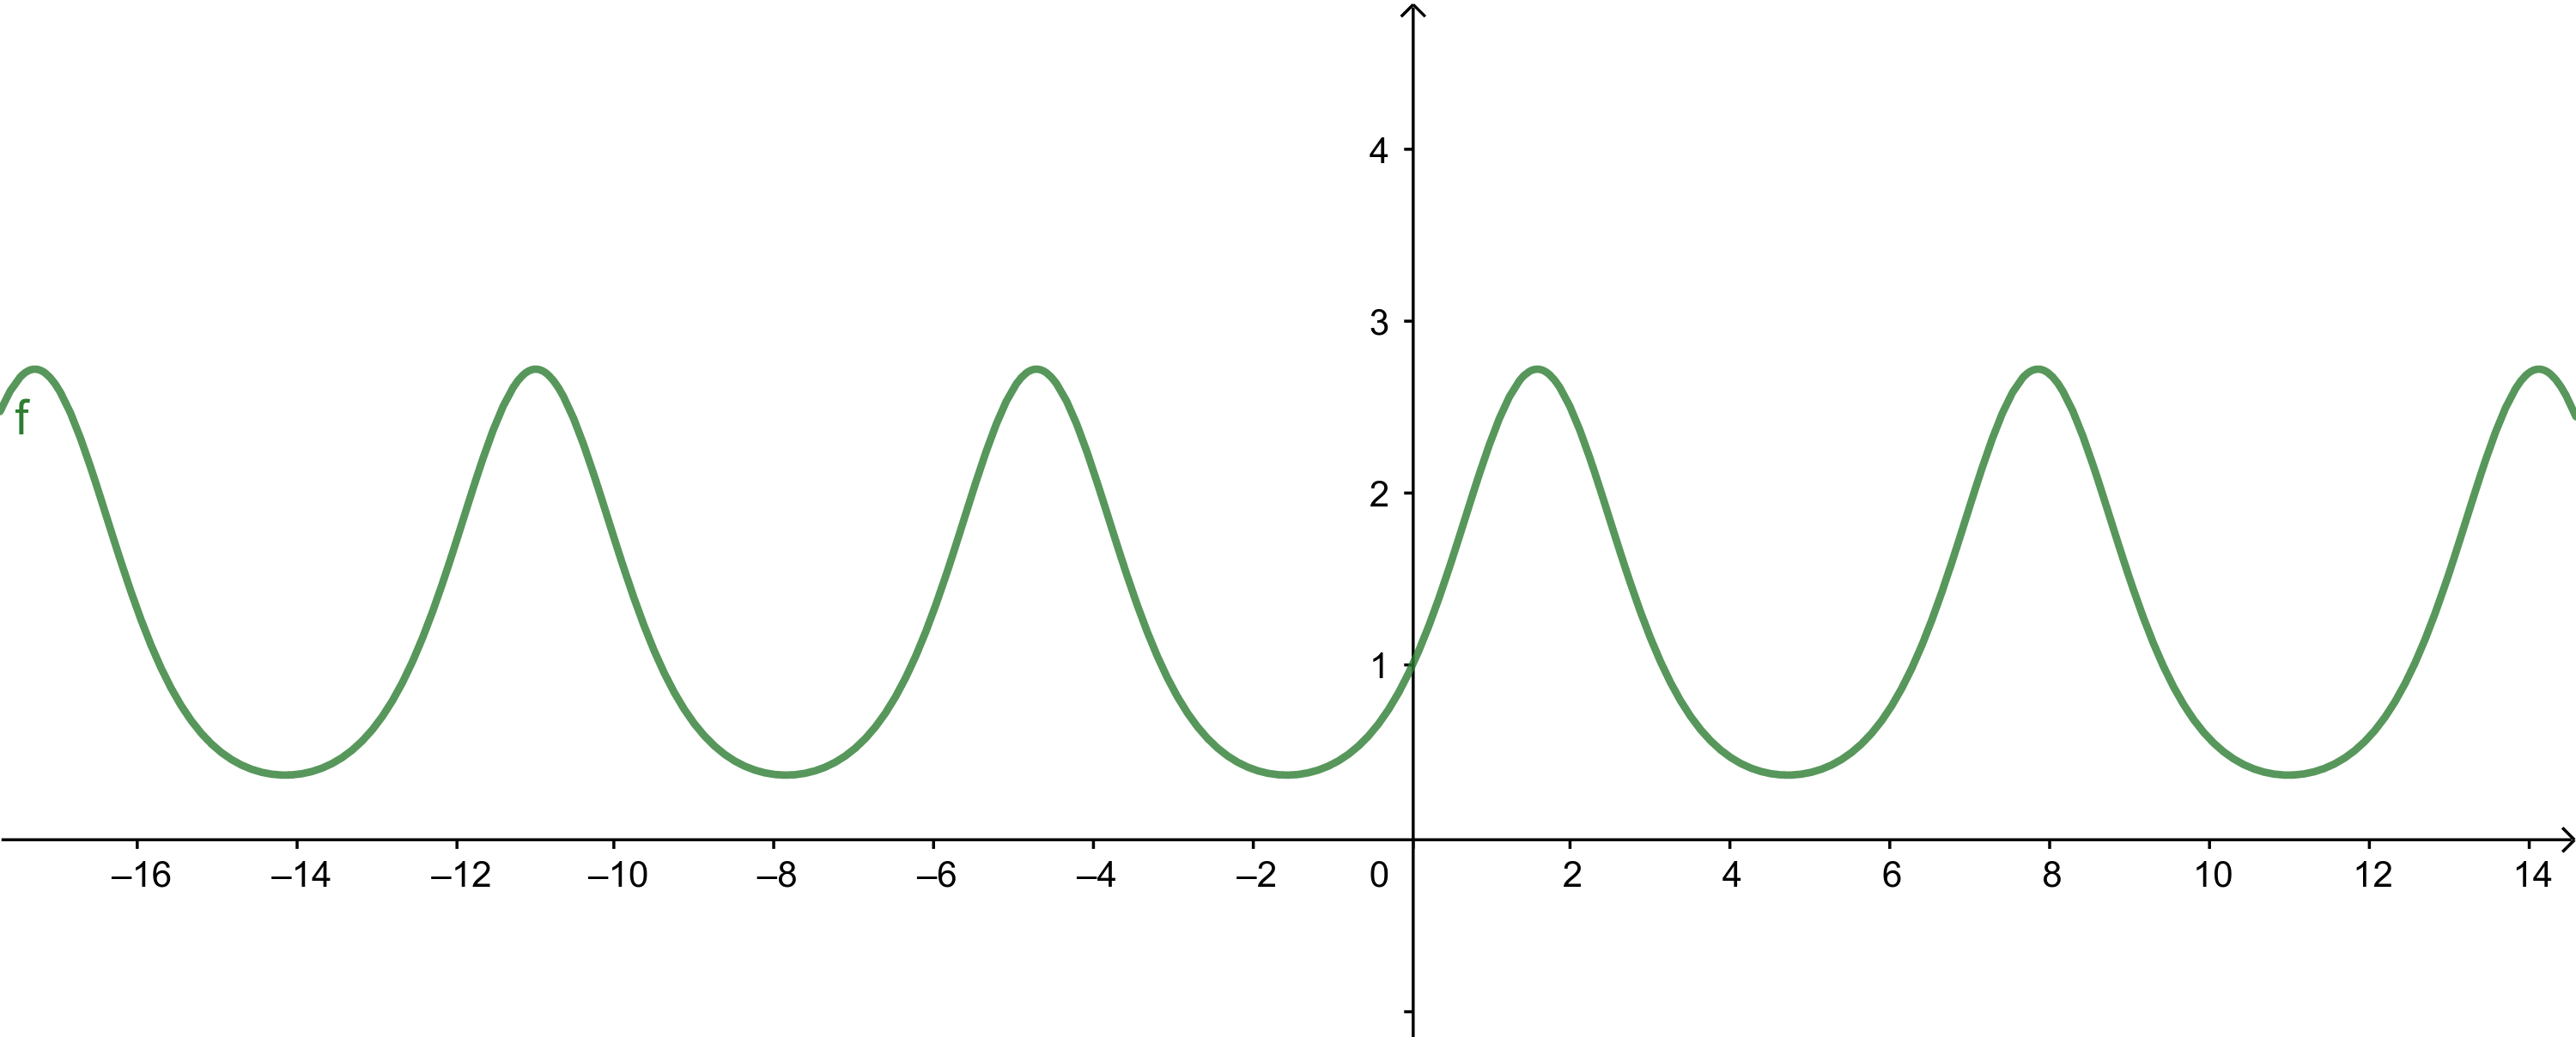
\includegraphics[width=0.5\textwidth]{15-b}
        \end{figure}

    %EJERCICIO C
    \item \(f(x)=e^x+e^{-x}\)\medskip
    
        \textbf{Continuidad: }\medskip

            \(e^x\) y \(e^{-x}\) son funciones continuas en todos los \(\mathbbm{R}\), por lo que su suma (\(e^x+e^{-x}\)), tambi\'en lo es.\medskip

        \textbf{Dominio: }\medskip

            Como no hay valores donde $f(x)$ est\'e indefinida: \(Dom(f):\mathbbm{R}\)\medskip

        \textbf{Imagen: }\medskip

            Como \(e^{-x}>0\), podemos decir que \(0<e^x<e^x+e^-x\), lo que significa que \(e^x\) est\'a por debajo de \(f\) y, como \(e^x\) no est\'a acotada superiormente, \(f\) tampoco lo est\'a. Analogo es el caso con \(0<e^{-x}<e^x+e^-x\). Por lo que sabemos que \(f\) no est\'a acotada superiormente y que est\'a entre \(e^x\) y \(e^{-x}\).\medskip

            En los puntos cr\'iticos demostraremos que: \(Img(f)=\{y\in\mathbbm{R} \ | \ y\geq2\}\)\medskip

        \textbf{Ra\'ices: }\medskip

            Como ya se dijo anteriormente, \(f\) est\'a entre \(e^x\) y \(e^{-x}\) y como cambas con mayores a 0, \(f(x)>0 \forall x \in \mathbbm{R}\), por lo que \(f\) no tiene ra\'ices.\medskip

        \textbf{Paridad: }
            \begin{equation*}
                f(-x) = e^{-x}+e^{-(-x)} = e^{-x}+e^x = e^x+e^{-x} = f(x) \qquad \text{(es par)}
            \end{equation*}

        \textbf{Derivadas: }
            \begin{equation*}
                f'(x) = \frac{d}{dx}\left(e^x+e^{-x}\right) = e^x(1)+e^{-x}(-1) = e^x-e^{-x}
            \end{equation*}

            \begin{equation*}
                f''(x) = \frac{d}{dx}\left(e^x-e^{-x}\right) = e^x(1)-e^{-x}(-1) = e^x+e^{-x}
            \end{equation*}

        \textbf{Puntos y valores cr\'iticos: }
            \begin{equation*}
                f'(x)=0 \Rightarrow e^x-e^{-x}=0 \Rightarrow e^x=e^{-x} \Rightarrow \ln(e^x)=\ln(e^{-x}) \Rightarrow x=-x
            \end{equation*}
            NOTA: Podemos aplicar logaritmo por ambos lados de la ecucaci\'on son siempre positivos.\medskip

            Como en los realies la premisa \(x = -x\) s\'olo se cumple con \(x=0\), por lo que 0 es el \'unico punto cr\'itico de \(f\)
            \begin{equation*}
                f(0)=e^0+e^{-0}=1+1=2 \Longrightarrow (0,2) \quad \text{Valor crítico}
            \end{equation*}

            Analizamos \(f''(0)\): \quad \(f''(0)=e^0+e^{-0}=1+1=2>0\) \(x=0\) es un m\'inimo.\medskip

            Sabiendo que \((0,2)\) es el \'unico punto cr\'itico que obtenemos, que la funci\'on est\'a entre \(e^x\) y \(e^{-x}\) (lo que significa que es mayor a 0), y que es par, podemos afirmar que el m\'inimo valor de \(f(x)\) es 2, as\'i entocnes la imagen de \(f\) es: \([2,\infty)\).

        \textbf{Crecencia: }
        \begin{equation*}
            f'(x)>0 \Rightarrow e^x-e^{-x}>0 \Rightarrow e^x>e^{-x} \Rightarrow \ln(e^x)>\ln(e^{-x}) \Rightarrow x>-x
        \end{equation*}

        Si \(x<0 \Rightarrow x>-x\Rightarrow\!\Leftarrow\) Porque \(-x>0\) y un negativo no puede ser mayor a un positivo.\medskip

        Si \(x>0 \Rightarrow x>-x\) La premisa se cumple. Por lo que \(f\) es creciente en \(x>0\) y, como la funci\'on es par, es decreciente en \(x<0\).\medskip

        \textbf{Puntos y valores de Inflexi\'on: }\medskip

            Sabemos que \(f''(x)=e^x+e^{-x}=f(x)\) y que \(f(x)\geq2>0\), por lo que \(f''(x)\) nunca es 0, asi entonces, la funci\'on no tiene puntos de inflexi\'on.\medskip

        \textbf{Concavidad y Convexidad: }

            Analogo a los puntos de inflexi\'on. Como \(f''(x)=f(x)\) y \(f(x)\geq2>0\), entonces \(f''(x)>0 \ \forall x\in\mathbbm{R}\), por lo que la funci\'on es siempre convexa.\medskip

        \textbf{Gr\'afica: }\medskip

        \begin{figure}[ht]
            \centering
            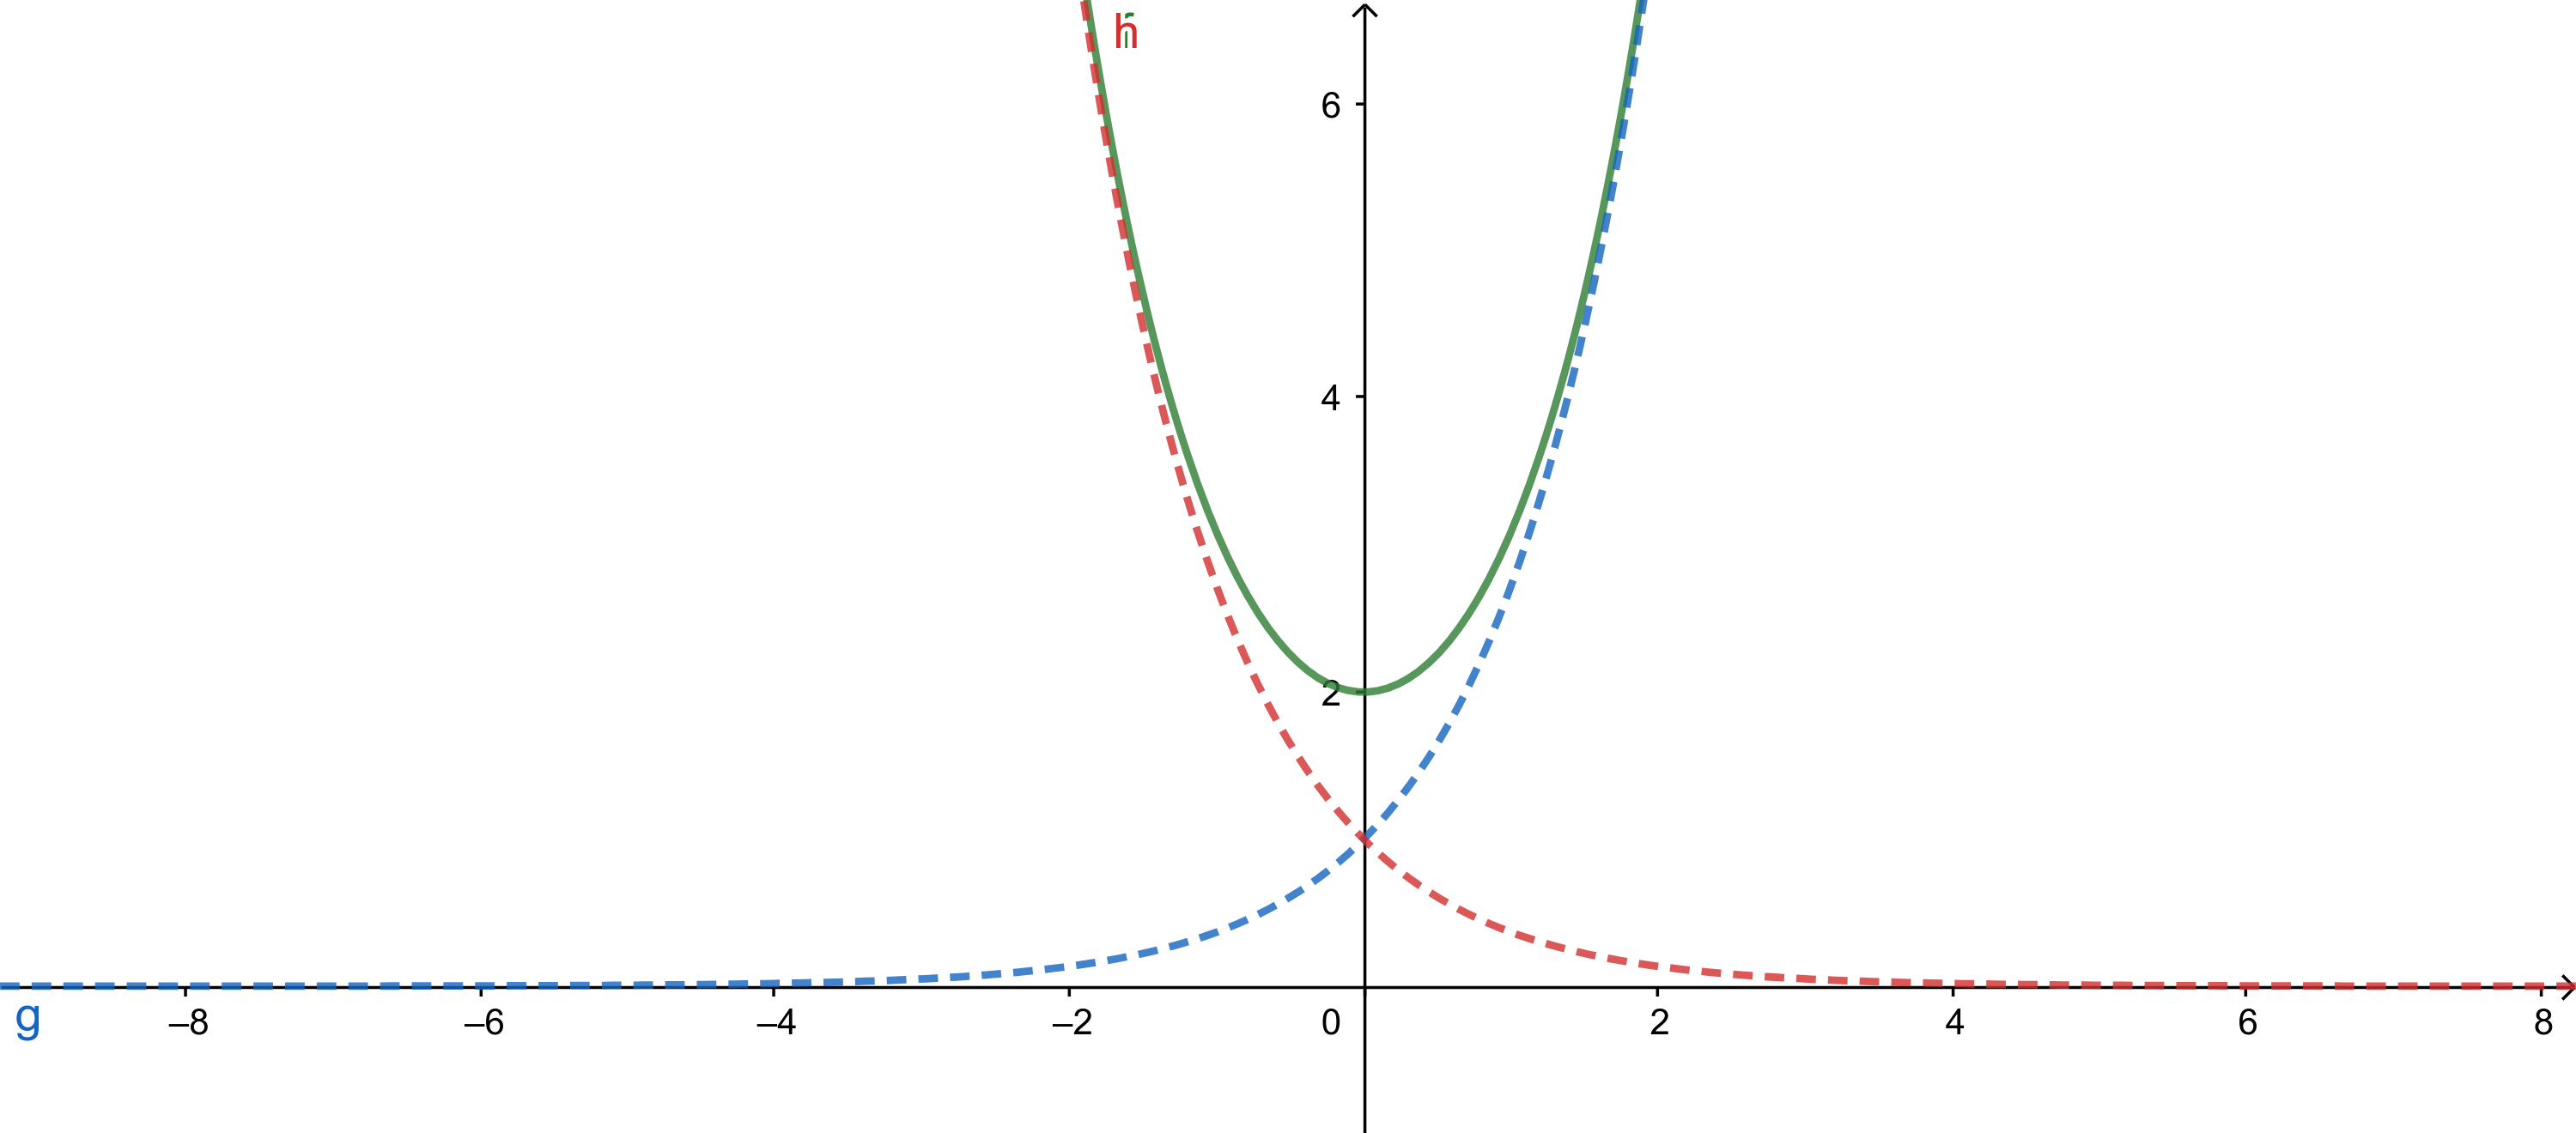
\includegraphics[width=0.5\textwidth]{15-c}
        \end{figure}

    %EJERCICIO D
    \item \(f(x)=e^x-e^{-x}\)\medskip
    
        \textbf{Continuidad: }\medskip

            \(e^x\) y \(e^{-x}\) son funciones continuas en todos los \(\mathbbm{R}\), por lo que su resta (\(e^x-e^{-x}\)), tambi\'en lo es.\medskip

        \textbf{Dominio: }\medskip

            Como no hay valores donde $f(x)$ est\'e indefinida: \(Dom(f):\mathbbm{R}\)\medskip

        \textbf{Imagen: }\medskip

            (Como m\'as adelante demostramos que la funci\'on es impar, nos centraremos solo en las \(x>0\)) Notemos que si \(x>0 \Rightarrow x>-x \Rightarrow e^x>e^{-x} \Rightarrow e^x-e^{-x}>0\)\medskip

            Sabiendo que \(\lim_{x\to\infty}e^x=\infty\), obtenemos su l\'imite al infinito:
            \begin{equation*}
                \lim_{x\to\infty}e^x-e^{-x}=\lim_{x\to\infty}e^x-\frac{1}{e^x}=\lim_{x\to\infty}e^x-\lim_{x\to\infty}\frac{1}{e^x} = \lim_{x\to\infty}e^x-0=\lim_{x\to\infty}e^x=\infty
            \end{equation*}

            Lo que significa que \(x\to0 \Rightarrow f(x)\to0\), por lo que la funci\'on no est\'a acotada en \(x>0\) y tiende a infinito. Dada la paritdad de la funci\'on, sabemos que tampoco est\'a acotada inferiormente y que tiene a \(-\infty\).\medskip

        \textbf{Ra\'ices: }
            \begin{equation*}
                f'(x)=0 \Rightarrow e^x-e^{-x}=0 \Rightarrow e^x=e^{-x} \Rightarrow \ln(e^x)=\ln(e^{-x}) \Rightarrow x=-x
            \end{equation*}
            NOTA: Podemos aplicar logaritmo por ambos lados de la ecucaci\'on son siempre positivos.\medskip

            Como en los realies la premisa \(x = -x\) s\'olo se cumple con \(x=0\), \(f\) tiene una \'unica ra\'iz en \(x=0\).
            \begin{equation*}
                f(0)=e^0-e^{-0}=1-1=0 \Longrightarrow (0,0) \quad \text{Raíz}
            \end{equation*}

        \textbf{Paridad: }
            \begin{equation*}
                f(-x) = e^{-x}-e^{-(-x)} = e^{-x}-e^{x} = -(e^x-e^{-x}) = -f(x) \qquad \text{(es impar)}
            \end{equation*}

        \textbf{Derivadas: }
            \begin{equation*}
                f'(x) = \frac{d}{dx}\left(e^x-e^{-x}\right) = e^x(1)-e^{-x}(-1) = e^x+e^{-x}
            \end{equation*}

            \begin{equation*}
                f''(x) = \frac{d}{dx}\left(e^x+e^{-x}\right) = e^x(1)+e^{-x}(-1) = e^x-e^{-x}
            \end{equation*}

        \textbf{Puntos y valores cr\'iticos: }\medskip

            \(f'(x)=0 \Rightarrow e^x+e^{-x}=0\)\quad Definimos \(e^x+e^{-x}\) en el ejercicio c y demostramos que \(e^x+e^{-x}\geq2 \ \forall x\in\mathbbm{R}\). Por lo que \(f'(x)\) nunca es 0, as\'i entonces, la funci\'on no tiene puntos cr\'iticos.\medskip

        \textbf{Crecencia: }\medskip

            Analogo al anterior, como en el ejericico c demostramos que \(e^x+e^{-x}\geq2 \ \forall x\in\mathbbm{R}\), as\'i \(f'(x)>0\), por lo que la funci\'on siempre es creciente.\medskip

        \textbf{Puntos y valores de Inflexi\'on: }\medskip

            Como \(f''(x)=e^x-e^{-x}=f(x)\) y ya demostramos que \(f(x)=0\) cuando \(x=0 \Rightarrow (0,0)\), \((0,0)\) es un valor de inflexi\'on.

        \textbf{Concavidad y Convexidad: }\medskip

            Como \(f''(x)=e^x-e^{-x}=f(x)\) y ya demostramos que cuando \(x>0 \Rightarrow f(x)>0\), la funci\'on es convexa en \((0,\infty)\), y, como es impar, es c\'oncava en \(x<0\).\medskip

        \textbf{Gr\'afica: }\medskip

        \begin{figure}[ht]
            \centering
            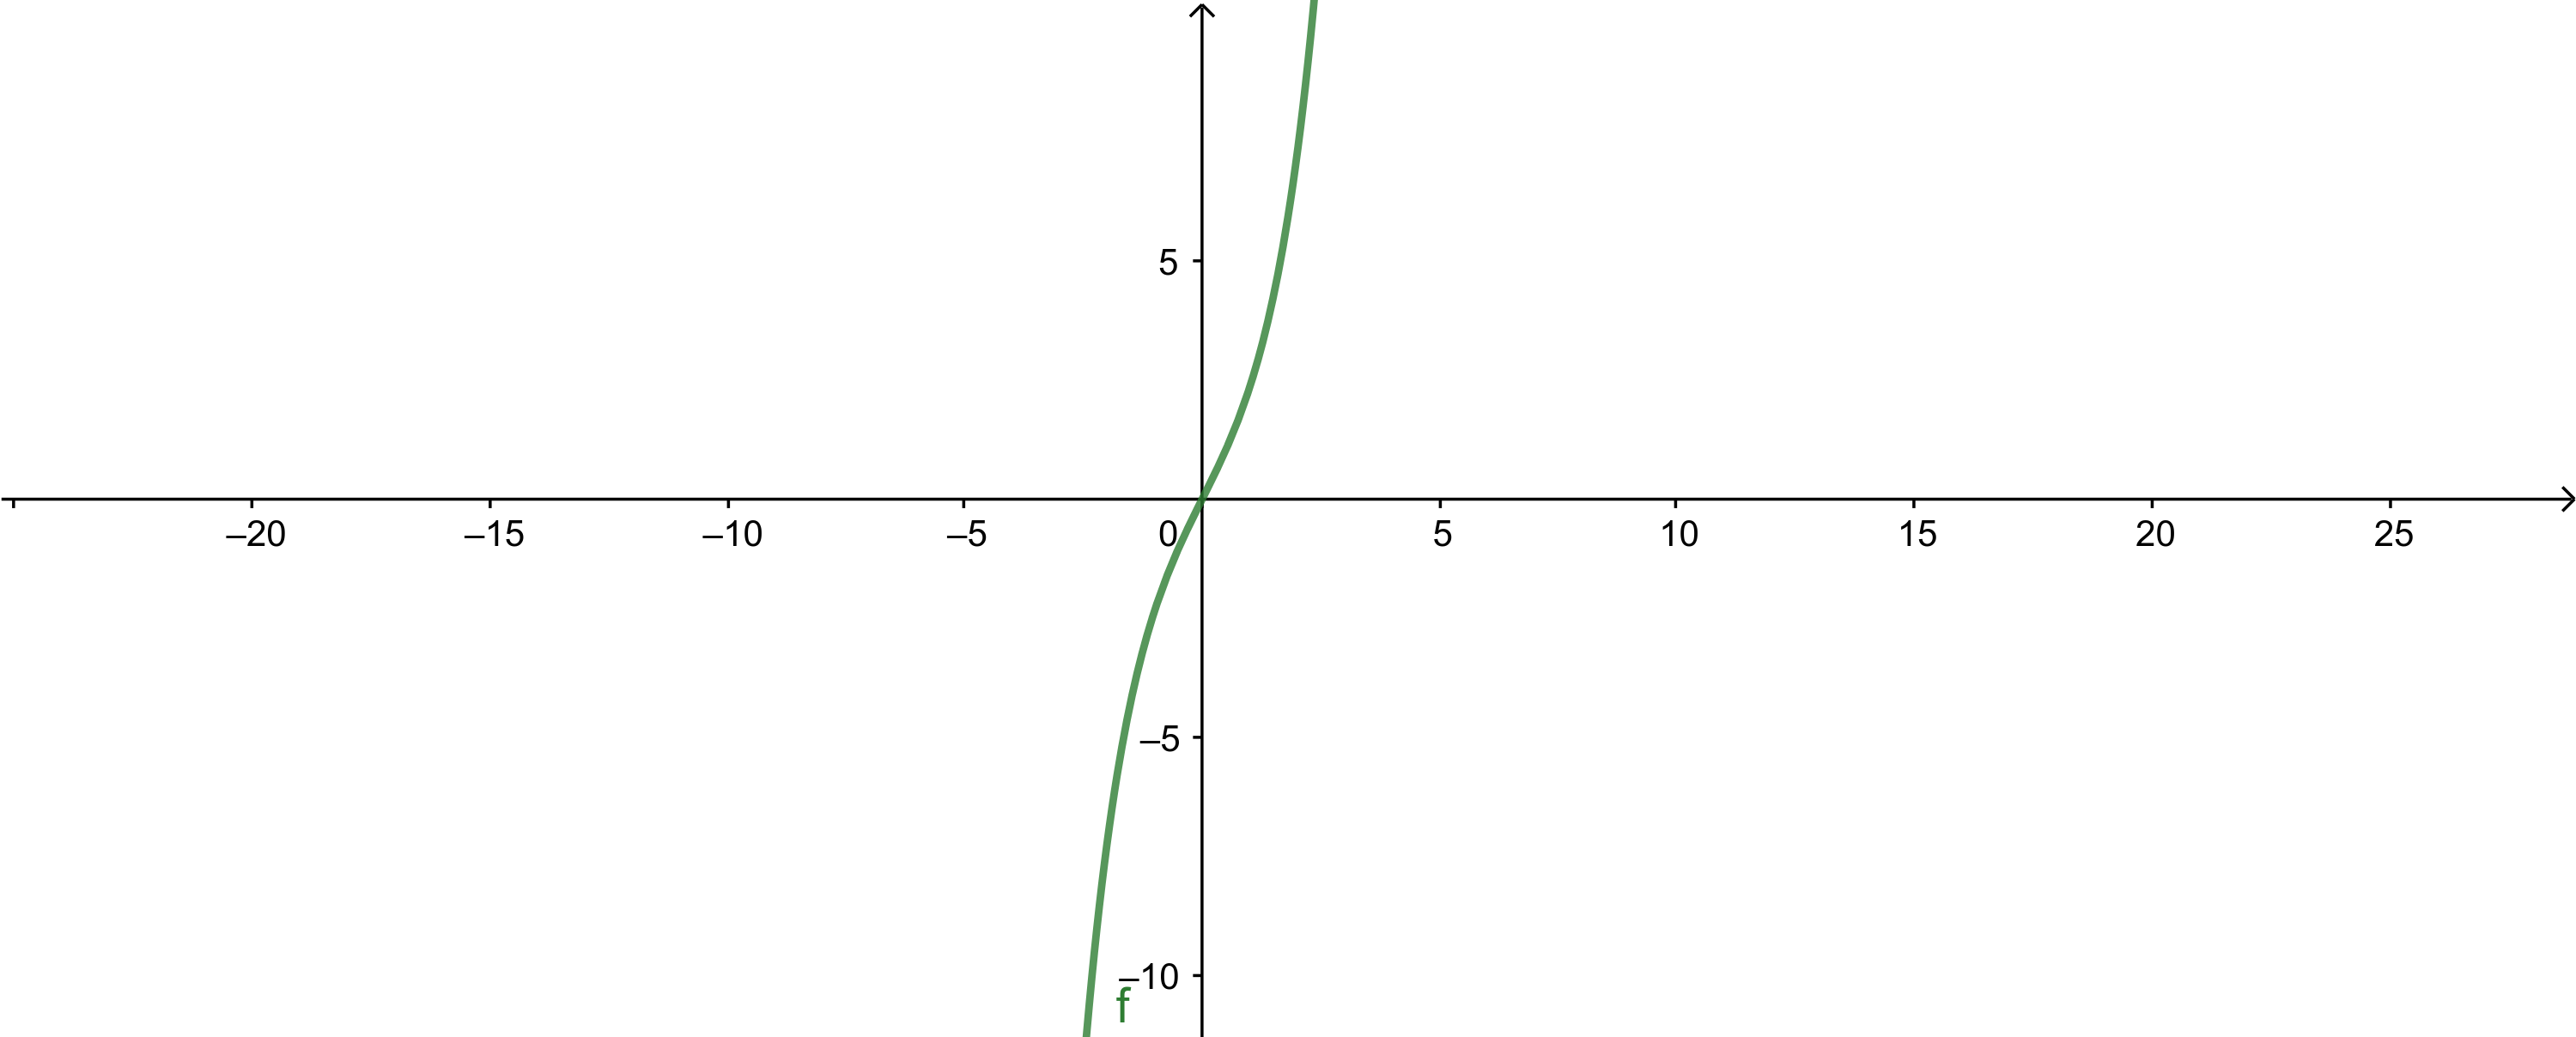
\includegraphics[width=0.5\textwidth]{15-d}
        \end{figure}

    %EJERCICIO E
    \item \(f(x)=\displaystyle\frac{e^x-e^{-x}}{e^x+e^{-x}}=1-\frac{2}{e^{2x}+1}\)\medskip
    
        \textbf{Continuidad: }\medskip

            Como \(f\) es una fracci\'on, el denominador no puede ser 0, es decir \(e^x+e^{-x}\neq0\), pero ya demostramos, en el inciso c, que \(e^x+e^{-x}\geq2>0\), por lo que la funci\'on, al ser una composici\'on de funciones continuas (demostrado en los incisos c y d) y no tener resstricciones, es continua en todos los \(\mathbbm{R}\).\medskip

        \textbf{Dominio: }\medskip

            Como no hay valores donde $f(x)$ est\'e indefinida: \(Dom(f):\mathbbm{R}\)\medskip

        \textbf{Imagen: }\medskip

            Sabemos que \(e^{2x}>0 \Rightarrow e^{2x}+1>1>0\) y, por lo tanto, que \(\displaystyle\frac{1}{e^{2x}+1}>0\). As\'i:
            \begin{align*}
                &e^{2x}+1>1 \Longrightarrow 0<\frac{1}{e^{2x}+1}<\frac{1}{1}=1 \Longrightarrow  0<\frac{2}{e^{2x}+1}<2 \\
                &\Longrightarrow  0>-\frac{2}{e^{2x}+1}>-2 \Longrightarrow  1+0>1-\frac{2}{e^{2x}+1}>1-2 \\ 
                &\Longrightarrow  1>1-\frac{2}{e^{2x}+1}>-1 \Longrightarrow \left|1-\frac{2}{e^{2x}+1}\right|<1
            \end{align*}

            As\'i, $f$  est\'a acotada por $M=1$, por lo que: \(Img(f): [-1,1]\)\medskip

        \textbf{Ra\'ices: }
            \begin{equation*}
                \frac{e^x-e^{-x}}{e^x+e^{-x}}=0 \Longrightarrow e^x-e^{-x}=0
            \end{equation*}

            Sabemos, por el inciso d, que \(e^x-e^{-x}=0\) en \(x=0\). Por lo que tenemos una ra\'iz en ese punto.\medskip

            \(f(0)=\frac{e^0-e^{-0}}{e^0+e^{-0}} = \frac{1-1}{1+1} = \frac{0}{2} = 0 \Longrightarrow (0,0) \quad \text{Raíz}\)

        \textbf{Paridad: }
            \begin{equation*}
                f(-x) = \frac{e^{-x}-e^{-(-x)}}{e^{-x}+e^{-(-x)}} = \frac{e^{-x}-e^x}{e^{-x}+e^x} = \frac{-(e^x-e^{-x})}{e^x+e^{-x}} = -f(x) \quad \text{(impar)}
            \end{equation*}

        \textbf{Derivadas: } \quad Utilizando derivaci\'on logar\'itmica:
            \begin{align*}
                f(x) &= \frac{e^x-e^{-x}}{e^x+e^{-x}} \Longrightarrow \ln(f(x)) = \ln\left(\frac{e^x-e^{-x}}{e^x+e^{-x}}\right)\\
                \frac{d}{dx}\ln(f(x))&=\frac{d}{dx}\ln\left(\frac{e^x-e^{-x}}{e^x+e^{-x}}\right)\\
                \frac{f'(x)}{f(x)}&=\frac{d}{dx}\left[\ln(e^x-e^{-x})-\ln(e^x+e^{-x})\right]\\
                &=\frac{\frac{d}{dx}(e^x-e^{-x})}{e^x-e^{-x}}-\frac{\frac{d}{dx}(e^x+e^{-x})}{e^x+e^{-x}}\\
                &=\frac{e^x+e^{-x}}{e^x-e^{-x}}-\frac{e^x-e^{-x}}{e^x+e^{-x}} \quad \text{(Incisos c y d)}\\
                f'(x)&= f(x)\left[\frac{e^x+e^{-x}}{e^x-e^{-x}}-\frac{e^x-e^{-x}}{e^x+e^{-x}}\right]\\
                &= \frac{e^x-e^{-x}}{e^x+e^{-x}}\left[\frac{e^x+e^{-x}}{e^x-e^{-x}}-\frac{e^x-e^{-x}}{e^x+e^{-x}}\right]\\
                &= \frac{e^x-e^{-x}}{e^x+e^{-x}}\cdot\frac{e^x+e^{-x}}{e^x-e^{-x}} - \frac{e^x-e^{-x}}{e^x+e^{-x}}\cdot\frac{e^x-e^{-x}}{e^x+e^{-x}}\\
                &= 1- \frac{(e^x-e^{-x})^2}{(e^x+e^{-x})^2} = \frac{(e^x+e^{-x})^2}{(e^x+e^{-x})^2} - \frac{(e^x-e^{-x})^2}{(e^x+e^{-x})^2}\\
                &= \frac{(e^x+e^{-x})^2-(e^x-e^{-x})^2}{(e^x+e^{-x})^2}\\
                &= \frac{(e^{2x}+2e^xe^{-x}+e^{-2x})-(e^{2x}-2e^xe^{-x}+e^{-2x})}{(e^x+e^{-x})^2}\\
                &= \frac{e^{2x}+2+e^{-2x}-e^{2x}+2-e^{-2x}}{(e^x+e^{-x})^2}\\
                f'(x)&= \frac{4}{(e^x+e^{-x})^2}
            \end{align*}

            \begin{align*}
                f''(x) &= \frac{d}{dx}\left[\frac{4}{(e^x+e^{-x})^2}\right] = 4\frac{d}{dx}\left[\frac{1}{(e^x+e^{-x})^2}\right] = 4 \frac{d}{dx}\left[(e^x+e^{-x})^{-2}\right]\\
                &= 4\frac{d}{dx}\left[(e^x+e^{-x})^{-2}\right]\frac{d}{dx}\left[(e^x+e^{-x})\right] = 4\cdot-2(e^x+e^{-x})^{-3}\cdot(e^x-e^{-x})\\
                &= -\frac{8(e^x-e^{-x})}{(e^x+e^{-x})^3}
            \end{align*}

        \textbf{Puntos y valores cr\'iticos: }\medskip

            \(f'(x)=0 \Longrightarrow \frac{4}{(e^x+e^{-x})^2}=0 \Longrightarrow 4=0\Rightarrow\!\Leftarrow\)\quad \(f\) no tiene puntos cr\'iticos porque \(f'(x)\) nunca es 0.\medskip

        \textbf{Crecencia: }\medskip

            \(f'(x)=\frac{4}{(e^x+e^{-x})^2}\). Como $4>0$ y $(e^x+e^{-x})^2>0$ (Por el cuadrado) \(f'(x)>0 \ \forall x\in \mathbbm{R}\). Por lo que $f$ es siempre creciente.\medskip

        \textbf{Puntos y valores de Inflexi\'on: }
            \[f''(x)=0 \Longrightarrow -\frac{8(e^x-e^{-x})}{(e^x+e^{-x})^3}=0 \Longrightarrow 8(e^x-e^{-x})=0 \Longrightarrow e^x-e^{-x}=0\]

            Por el inciso d sabemos que \(e^x-e^{-x}=0\) cuando \(x=0 \Longrightarrow f(0)=0\), as\'i pues, $f$ tiene un punto de inflexi\'on en \((0,0)\).\medskip

        \textbf{Concavidad y Convexidad: }\medskip
            \[f''(x)>0 \Longrightarrow -\frac{8(e^x-e^{-x})}{(e^x+e^{-x})^3}>0 \Longrightarrow \frac{8(e^x-e^{-x})}{(e^x+e^{-x})^3}<0\]

            Sabemos, por el inciso c, que \(e^x+e^{-x}>0 \Longrightarrow (e^x+e^{-x})^3>0\), por lo que \(f''(x)\) ser\'a mayor a 0 s\'olo cuando \(8(e^x-e^{-x})<0 \Longrightarrow e^x-e^{-x}<0\).\medskip

            Sabemos tambi\'en, por el inciso d, que \(e^x-e^{-x}<0\) cuando \(x<0\). Por lo que \(f''(x)>0\) ($f$ es convexa) cuando \(x<0\).\medskip

            Como la funci\'on es impar, es c\'oncava en \(x>0\).\medskip

        \textbf{Gr\'afica: }\medskip

        \begin{figure}[ht]
            \centering
            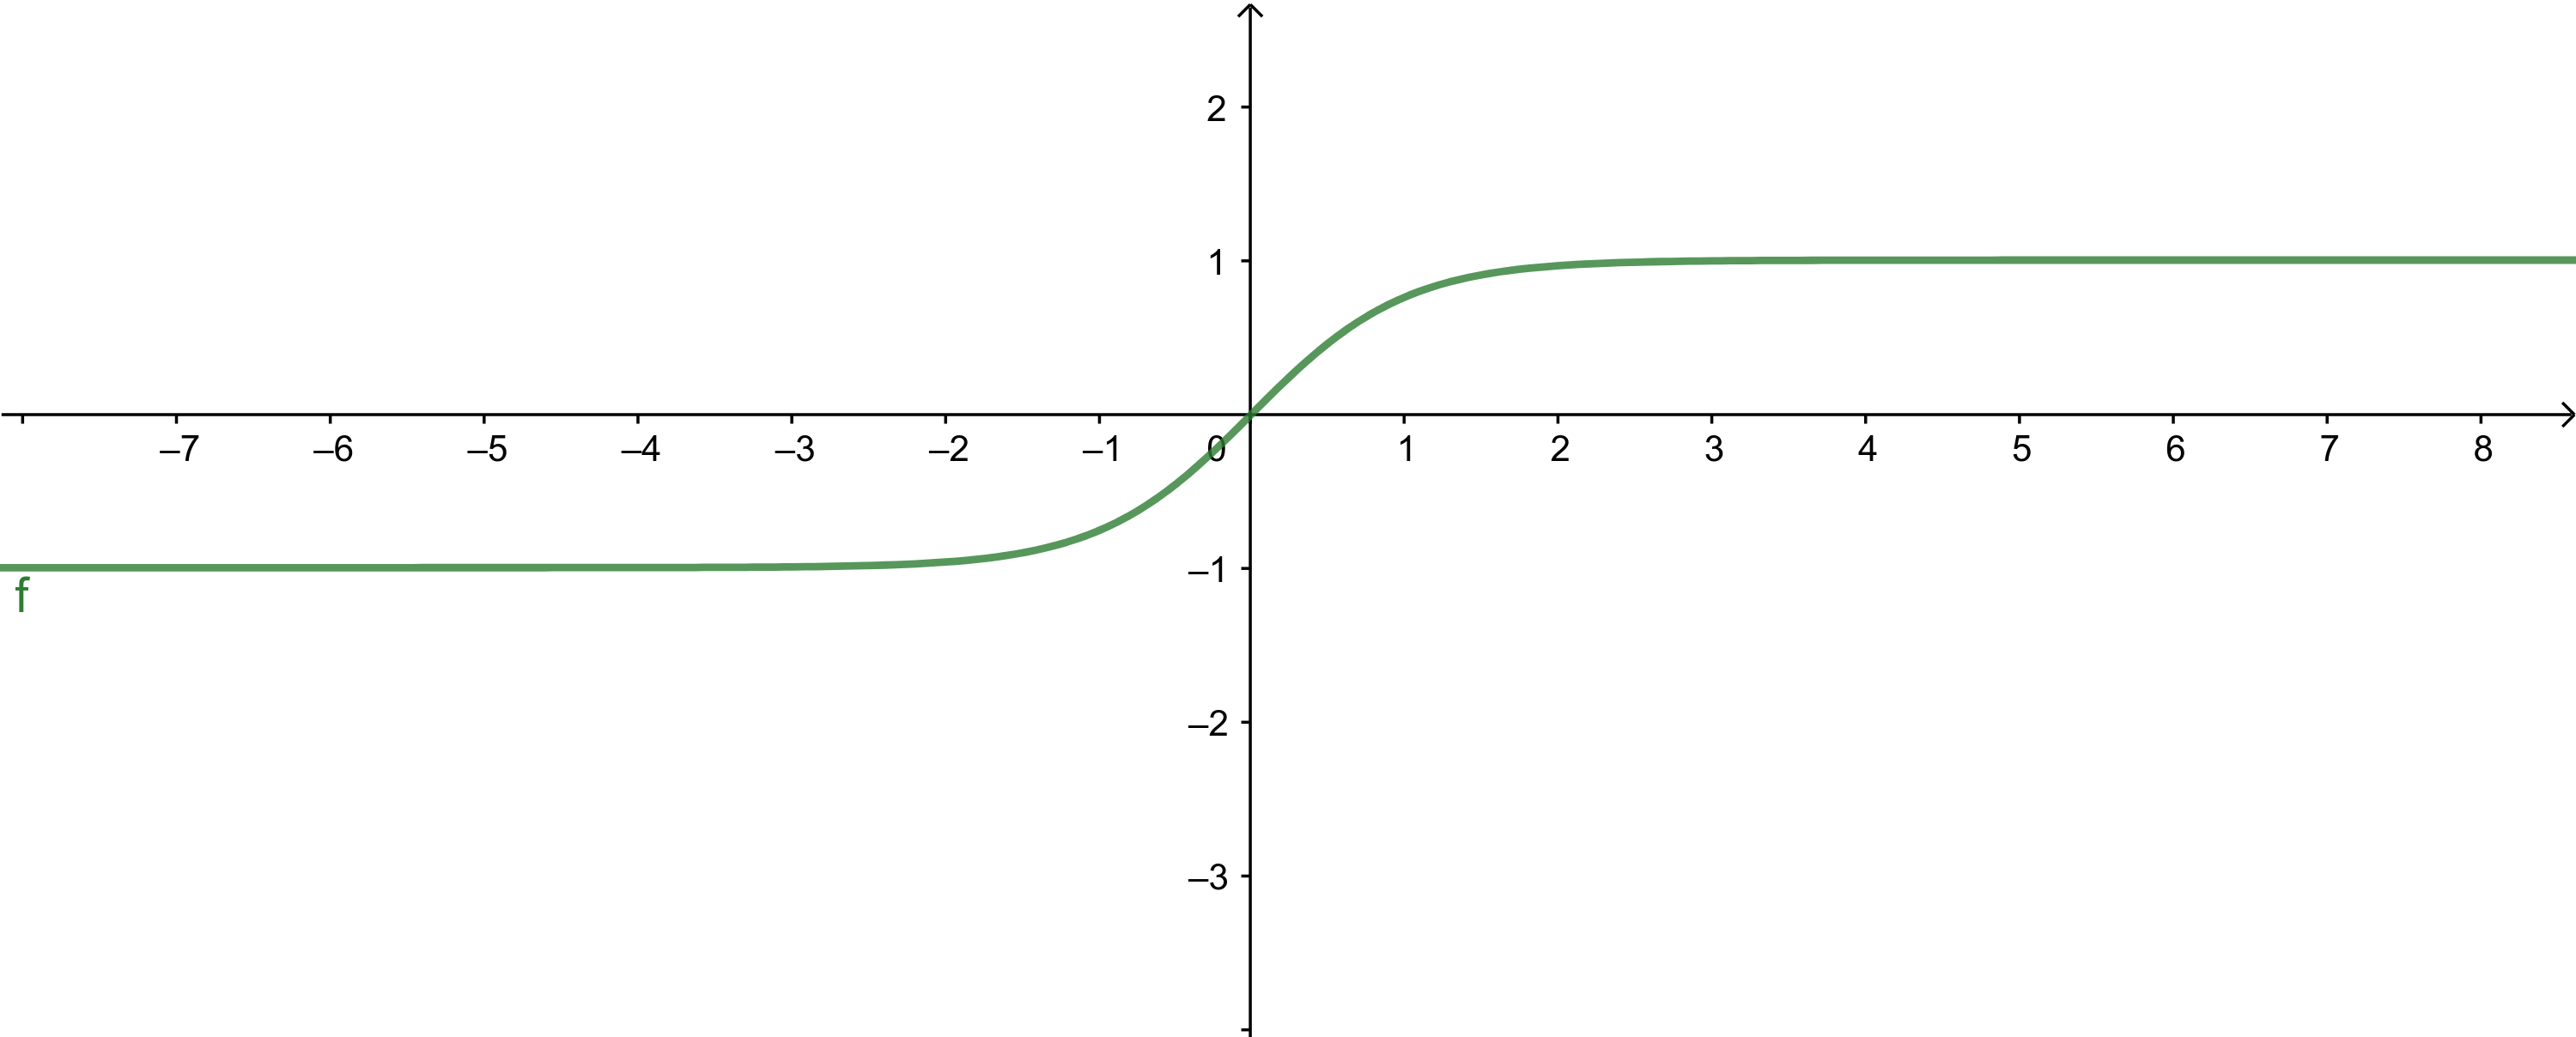
\includegraphics[width=0.5\textwidth]{15-e}
        \end{figure}

\end{enumerate}

%EJERCICIO 16 ----------------------------------------------------------------------------------
16. Las siguientes funciones reciben el nombre de seno hiperb\'olico, coseno hiperb\'olico y tangente hiperb\'olica, respectivamente.

\begin{equation*}
    \sinh(x)=\frac{e^x-e^{-x}}{2}, \ \cosh(x)=\frac{e^x+e^{-x}}{2} \ y \ \tanh(x)=\frac{e^x-e^{-x}}{e^x+e^{-x}}
\end{equation*}

Mostrar que:

\begin{enumerate}[\hspace{9px} a)]
    %EJERCICIO A
    \item \(\cosh^2(x)-\sinh^2(x)=1\)
    
        \begin{proof}[Prueba:]
            \begin{align*}
                \cosh^2(x)-\sinh^2(x) &= \left(\frac{e^x+e^{-x}}{2}\right)^2-\left(\frac{e^x-e^{-x}}{2}\right)^2 = \frac{(e^x+e^{-x})^2}{4} - \frac{(e^x-e^{-x})^2}{4}\\
                &= \frac{(e^x+e^{-x})^2-(e^x-e^{-x})^2}{4} \\
                &= \frac{e^{2x}+2e^xe^{-x}+e^{-2x}-e^{2x}+2e^xe^{-x}-e^{-2x}}{4}\\
                &= \frac{4e^{x-x}}{4} = \frac{4e^0}{4} = \frac{4(1)}{4} = 1
            \end{align*}
        \end{proof}

    %EJERCICIO B
    \item \(\sinh'(x)=\cosh(x)\)
    
        \begin{proof}[Prueba:]
            \begin{align*}
                \frac{d}{dx}\sinh(x) &= \frac{d}{dx}\left[\frac{e^x-e^{-x}}{2}\right] = \frac{1}{2}\cdot\frac{d}{dx}(e^x-e^{-x})\\
                &= \frac{1}{2}(e^x(1)-e^{-x}(-1)) = \frac{e^x+e^{-x}}{2} = \cosh(x)
            \end{align*}
        \end{proof}

    %EJERCICIO C
    \item \(\cosh'(x)=\sinh(x)\) 
    
        \begin{proof}[Prueba:]
            \begin{align*}
                \frac{d}{dx}\cosh(x) &= \frac{d}{dx}\left[\frac{e^x+e^{-x}}{2}\right] = \frac{1}{2}\cdot\frac{d}{dx}(e^x+e^{-x})\\
                &= \frac{1}{2}(e^x(1)+e^{-x}(-1)) = \frac{e^x-e^{-x}}{2} = \sinh(x)
            \end{align*}
        \end{proof}

    %EJERCICIO D
    \item \(\tanh^2(x)+\displaystyle\frac{1}{\cosh^2(x)}=1\)
    
    \begin{proof}[Prueba:]
        \begin{equation*}
            \tanh(x) = \frac{e^x-e^{-x}}{e^x+e^{-x}} = \frac{e^x-e^{-x}}{e^x+e^{-x}}\cdot\frac{1/2}{1/2} = \frac{\displaystyle\frac{e^x-e^{-x}}{2}}{\displaystyle\frac{e^x+e^{-x}}{2}} = \frac{\sinh(x)}{\cosh(x)}
        \end{equation*}

        \begin{multline*}
            \tanh^2(x)+\frac{1}{\cosh^2(x)} = \left(\frac{\sinh(x)}{\cosh(x)}\right)^2+\frac{1}{\cosh^2(x)} \\ = \frac{\sinh^2(x)}{\cosh^2(x)}+\frac{1}{\cosh^2(x)} = \frac{\sinh^2(x)+1}{\cosh^2(x)}
        \end{multline*}

        Recordando el inciso a: \(\cosh^2(x)-\sinh^2(x)=1\). Si despejamos \(\cosh^2(x)\) obtenemos: 
        \[\cosh^2(x) = 1+\sinh^2(x)\]

        Sustituyendo:

        \begin{equation*}
            \frac{\sinh^2(x)+1}{\cosh^2(x)} = \frac{\cosh^2(x)}{\cosh^2(x)} = 1
        \end{equation*}
    \end{proof}

    %EJERCICIO E
    \item \(\tanh'(x)=\displaystyle\frac{1}{\cosh^2(x)}\)
    
    \begin{proof}[Prueba:]
        \begin{align*}
            \tanh(x)=\frac{\sinh(x)}{\cosh(x)} \quad \text{(Demostrado en el inciso c)}
        \end{align*}

        Usando derivaci\'on logar\'itmica:
        \begin{align*}
            \ln(\tanh(x)) &= \ln\left(\frac{\sinh(x)}{\cosh(x)}\right) = \ln(\sinh(x))-\ln(\cosh(x))\\
            \frac{d}{dx}\big(\ln(\tanh(x))\big) &= \frac{d}{dx}\big[\ln(\sinh(x))-\ln(\cosh(x))\big]\\
            \frac{\tanh'(x)}{\tanh(x)} &= \frac{\sinh'(x)}{\sinh(x)} - \frac{\cosh'(x)}{\cosh(x)} =\frac{\cosh(x)}{\sinh(x)} - \frac{\sinh(x)}{\cosh(x)}\\
            \tanh'(x) &= \tanh(x)\left[\frac{\cosh(x)}{\sinh(x)} - \frac{\sinh(x)}{\cosh(x)}\right] = \frac{\sinh(x)}{\cosh(x)}\left[\frac{\cosh(x)}{\sinh(x)} - \frac{\sinh(x)}{\cosh(x)}\right]\\
            &= \frac{\sinh(x)}{\cosh(x)}\cdot\frac{\cosh(x)}{\sinh(x)} - \frac{\sinh(x)}{\cosh(x)}\cdot\frac{\sinh(x)}{\cosh(x)} = 1-\frac{\sinh^2(x)}{\cosh^2(x)}\\
            &= \frac{\cosh^2(x)}{\cosh^2(x)} - \frac{\sinh^2(x)}{\cosh^2(x)} = \frac{\cosh^2(x)-\sinh^2(x)}{\cosh^2(x)}\\
            &= \frac{1}{\cosh^2(x)} \quad \text{(Por el inciso a)}
        \end{align*}
    \end{proof}


    %EJERCICIO F
    \item \(\sinh(x+y)=\sinh(x)\cosh(y)+\sinh(y)\cosh(x)\)
    
    \begin{proof}[Prueba:]
        \begin{align*}
            \sinh(x+y) &= \frac{e^{x+y}-e^{-(x+y)}}{2} = \frac{e^{x+y}-e^{-(x+y)}}{2}\cdot\frac{2}{2} = \frac{2e^{x+y}-2e^{-(x+y)}}{4} \\
            &= \frac{2e^xe^y-2e^{-x}e^{-y}+0+0}{4}\\
            &= \frac{2e^xe^y-2e^{-x}e^{-y}+(e^{x-y}-e^{x-y})+(e^{y-x}-e^{y-x})}{4}\\
            &= \frac{(e^xe^y-e^{-x}e^{-y}+e^{x-y}-e^{y-x})+(e^xe^y-e^{-x}e^{-y}-e^{x-y}+e^{y-x})}{4}\\
            &= \frac{(e^xe^y-e^{-x}e^{-y}+e^xe^{-y}-e^ye^{-x})+(e^xe^y-e^{-x}e^{-y}-e^xe^{-y}+e^ye^{-x})}{4}\\
            &= \frac{[e^x(e^y+e^{-y})-e^{-x}(e^y+e^{-y})]+[e^x(e^y-e^{-y})+e^{-x}(e^y-e^{-y})]}{4}\\
            &= \frac{[(e^x-e^{-x})(e^y+e^{-y})]+[(e^x+e^{-x})(e^y-e^{-y})]}{4}\\
            &= \frac{(e^x-e^{-x})(e^y+e^{-y})}{4}+\frac{(e^x+e^{-x})(e^y-e^{-y})}{4}\\
            &= \frac{e^x-e^{-x}}{2}\cdot\frac{e^y+e^{-y}}{2}+\frac{e^x+e^{-x}}{2}\cdot\frac{e^y-e^{-y}}{2}\\
            &= \sinh(x)\cosh(y)+\cosh(x)\sinh(y)
        \end{align*}
    \end{proof}

    %EJERCICIO G
    \item \(\cosh(x+y)=\cosh(x)\cosh(y)+\sinh(y)\sinh(x)\)
    
    \begin{proof}[Prueba:]
        \begin{align*}
            \cosh(x+y) &= \frac{e^{x+y}+e^{-(x+y)}}{2} = \frac{e^{x+y}+e^{-(x+y)}}{2}\cdot\frac{2}{2} = \frac{2e^{x+y}+2e^{-(x+y)}}{4}\\
            &= \frac{2e^xe^y+2e^{-x}e^{-y}+0+0}{4}\\
            &= \frac{2e^xe^y+2e^{-x}e^{-y}+(e^{x-y}-e^{x-y})+(e^{y-x}-e^{y-x})}{4}\\
            &= \frac{(e^xe^y+e^{-x}e^{-y}+e^{x-y}+e^{y-x})+(e^xe^y+e^{-x}e^{-y}-e^{x-y}-e^{y-x})}{4}\\
            &= \frac{(e^xe^y+e^{-x}e^{-y}+e^xe^{-y}+e^ye^{-x})+(e^xe^y+e^{-x}e^{-y}-e^xe^{-y}-e^ye^{-x})}{4}\\
            &= \frac{[e^x(e^y+e^{-y})+e^{-x}(e^y+e^{-y})]+[e^x(e^y-e^{-y})-e^{-x}(e^y-e^{-y})]}{4}\\
            &= \frac{[(e^x+e^{-x})(e^y+e^{-y})]+[(e^x-e^{-x})(e^y-e^{-y})]}{4}\\
            &= \frac{(e^x+e^{-x})(e^y+e^{-y})}{4}+\frac{(e^x-e^{-x})(e^y-e^{-y})}{4}\\
            &= \frac{e^x+e^{-x}}{2}\cdot\frac{e^y+e^{-y}}{2}+\frac{e^x-e^{-x}}{2}\cdot\frac{e^y-e^{-y}}{2}\\
            &= \cosh(x)\cosh(y)+\sinh(x)\sinh(y)
        \end{align*}
    \end{proof}

\end{enumerate}

%EJERCICIO 17 ----------------------------------------------------------------------------------
17. ELIMINADO.\medskip

%EJERCICIO 18 ----------------------------------------------------------------------------------
18. Evalua los l\'imites usando la regla de L'H\^opital.

\begin{enumerate}[\hspace{9px} a)]
    %EJERCICIO A
    \item \(\displaystyle\lim_{x \to 0}\frac{e^x-1-x-\frac{x^2}{2}}{x^2}\)\bigskip
    
        \begin{equation*}
            \lim_{x \to 0}\frac{e^x-1-x-\frac{x^2}{2}}{x^2} = \frac{e^0-1-0-\frac{0^2}{2}}{0^2} = \frac{1-1}{0} = \frac{0}{0}
        \end{equation*}

        Como el l\'imite se indetermina en \(\displaystyle\frac{0}{0}\), comprobamos el l\'imite de las derivadas para poder utilizar L'H\^opital:

        \begin{equation*}
            \frac{d}{dx}\left(e^x-1-x-\frac{x^2}{2}\right) = e^x-1-\frac{1}{2}\cdot2x = e^x-1-x \qquad \quad \frac{d}{dx}x^2=2x
        \end{equation*}

        \begin{equation*}
            \lim_{x \to 0}\frac{e^x-1-x}{2x} = \frac{e^0-1-0}{2(0)} = \frac{1-1}{0} = \frac{0}{0}
        \end{equation*}

        Dado que el l\'imite de volvio a indeterminar en \(\displaystyle\frac{0}{0}\), volvemos a probar el l\'imite de las derivadas:

        \begin{equation*}
            \frac{d}{dx}(e^x-1-x) = e^x-1 \qquad \quad \frac{d}{dx}2x = 2
        \end{equation*}

        \begin{equation*}
            \lim_{x \to 0}\frac{e^x-1}{2} = \frac{e^0-1}{2} = \frac{1-1}{2} = \frac{0}{2} = 0
        \end{equation*}

        Como el l\'imite de las derivadas existe, podemos decir que el l\'imite existe y que:
        \begin{equation*}
            \lim_{x \to 0}\frac{e^x-1-x-\frac{x^2}{2}}{x^2} = \lim_{x \to 0}\frac{e^x-1-x}{2x} = \lim_{x \to 0}\frac{e^x-1}{2} = 0
        \end{equation*}

    %EJERCICIO B
    \item \(\displaystyle\lim_{x \to 0}\frac{e^x-1-x-\frac{x^2}{2}-\frac{x^3}{6}}{x^3}\)
    
        \begin{equation*}
            \lim_{x \to 0}\frac{e^x-1-x-\frac{x^2}{2}-\frac{x^3}{6}}{x^3} = \frac{e^0-1-0-\frac{0^2}{2}-\frac{0^3}{6}}{0^3} = \frac{1-1}{0} = \frac{0}{0}
        \end{equation*}

        Como el l\'imite se indetermina en \(\displaystyle\frac{0}{0}\), comprobamos el l\'imite de las derivadas para poder utilizar L'H\^opital:

        \begin{equation*}
            \frac{d}{dx}\left(e^x-1-x-\frac{x^2}{2}-\frac{x^3}{6}\right) = e^x-1-\frac{1}{2}\cdot2x-\frac{1}{6}\cdot3x^2 = e^x-1-x-\frac{x^2}{2} \qquad \quad \frac{d}{dx}x^3=3x^2
        \end{equation*}

        \begin{equation*}
            \lim_{x \to 0}\frac{e^x-1-x-\frac{x^2}{2}}{3x^2} = \frac{e^0-1-0-\frac{0^2}{2}}{2(0)^2} = \frac{1-1}{0} = \frac{0}{0}
        \end{equation*}

        Dado que el l\'imite de volvio a indeterminar en \(\displaystyle\frac{0}{0}\), volvemos a probar el l\'imite de las derivadas:

        \begin{equation*}
            \frac{d}{dx}(e^x-1-x-\frac{x^2}{2}) = e^x-1-x \qquad \quad \frac{d}{dx}3x^2 = 6x
        \end{equation*}

        \begin{equation*}
            \lim_{x \to 0}\frac{e^x-1-x}{6x} = \frac{e^0-1-0}{6(0)} = \frac{1-1}{0} = \frac{0}{0}
        \end{equation*}

        De nuevo, el l\'imite indetermin\'o en \(\displaystyle\frac{0}{0}\), por lo que volvemos a probar el l\'imite de las derivadas:

        \begin{equation*}
            \frac{d}{dx}(e^x-1-x) = e^x-1 \qquad \quad \frac{d}{dx}6x = 6
        \end{equation*}

        \begin{equation*}
            \lim_{x \to 0}\frac{e^x-1}{6} = \frac{e^0-1}{6} = \frac{1-1}{6} = \frac{0}{6} = 0
        \end{equation*}

        Como el l\'imite de las derivadas existe, podemos decir que el l\'imite existe y que:
        \begin{equation*}
            \lim_{x \to 0}\frac{e^x-1-x-\frac{x^2}{2}-\frac{x^3}{6}}{x^3} =  \lim_{x \to 0}\frac{e^x-1-x-\frac{x^2}{2}}{3x^2} = \lim_{x \to 0}\frac{e^x-1-x}{6x} =  \lim_{x \to 0}\frac{e^x-1}{6} = 0
        \end{equation*}

    %EJERCICIO C
    \item \(\displaystyle\lim_{x \to 0}\frac{e^x-1-x-\frac{x^2}{2}}{x^3}\)
    
        \begin{equation*}
            \lim_{x \to 0}\frac{e^x-1-x-\frac{x^2}{2}}{x^2} = \frac{e^0-1-0-\frac{0^2}{2}}{0^2} = \frac{1-1}{0} = \frac{0}{0}
        \end{equation*}

        Como el l\'imite se indetermina en \(\displaystyle\frac{0}{0}\), comprobamos el l\'imite de las derivadas para poder utilizar L'H\^opital:

        \begin{equation*}
            \frac{d}{dx}(e^x-1-x-\frac{x^2}{2}) = e^x-1-(\frac{1}{2}\cdot2x) = e^x-1-x \qquad \quad \frac{d}{dx}x^2=2x
        \end{equation*}

        \begin{equation*}
            \lim_{x \to 0}\frac{e^x-1-x}{2x} = \frac{e^0-1-0}{2(0)} = \frac{1-1}{0} = \frac{0}{0}
        \end{equation*}

        Dado que el l\'imite de volvio a indeterminar en \(\displaystyle\frac{0}{0}\), volvemos a probar el l\'imite de las derivadas:

        \begin{equation*}
            \frac{d}{dx}(e^x-1-x) = e^x-1 \qquad \quad \frac{d}{dx}2x = 2
        \end{equation*}

        \begin{equation*}
            \lim_{x \to 0}\frac{e^x-1}{2} = \frac{e^0-1}{2} = \frac{1-1}{2} = \frac{0}{2} = 0
        \end{equation*}

        Como el l\'imite de las derivadas existe, podemos decir que:
        \begin{equation*}
            \lim_{x \to 0}\frac{e^x-1-x-\frac{x^2}{2}}{x^2} = \lim_{x \to 0}\frac{e^x-1-x}{2x} = \lim_{x \to 0}\frac{e^x-1}{2} = 0
        \end{equation*}

    %EJERCICIO D
    \item \(\displaystyle\lim_{x \to 0}\frac{\ln(1+x)-x-\frac{x^2}{2}}{x^2}\)
        
        \begin{equation*}
            \lim_{x \to 0}\frac{\ln(1+x)-x-\frac{x^2}{2}}{x^2} = \frac{\ln(1+0)-0-\frac{0^2}{2}}{0^2} = \frac{\ln(1)}{0} = \frac{0}{0}
        \end{equation*}

        Como el l\'imite se indetermina en \(\displaystyle\frac{0}{0}\), comprobamos el l\'imite de las derivadas para poder utilizar L'H\^opital:

        \begin{equation*}
            \frac{d}{dx}\left(\ln(1+x)-x-\frac{x^2}{2}\right) = \frac{1}{1+x}-1-x \qquad \quad \frac{d}{dx}x^2=2x
        \end{equation*}

        \begin{equation*}
            \lim_{x \to 0}\frac{\frac{1}{1+x}-1-x}{2x} = \frac{\frac{1}{1+0}-1-0}{2(0)} = \frac{1-1}{0} = \frac{0}{0}
        \end{equation*}

        Dado que el l\'imite de volvio a indeterminar en \(\displaystyle\frac{0}{0}\), volvemos a probar el l\'imite de las derivadas:

        \begin{equation*}
            \frac{d}{dx}\left(\frac{1}{1+x}-1-x\right)= -\frac{1}{(1+x)^2}-1 \qquad \quad \frac{d}{dx}2x=2
        \end{equation*}

        \begin{equation*}
            \lim_{x \to 0}\frac{-\frac{1}{(1+x)^2}-1}{2} = \frac{-\frac{1}{(1+0)^2}-1}{2} = \frac{-1-1}{2} = -\frac{2}{2} = -1
        \end{equation*}

        Como el l\'imite de las derivadas existe, podemos decir que:

        \begin{equation*}
            \lim_{x \to 0}\frac{\ln(1+x)-x-\frac{x^2}{2}}{x^2} =  \lim_{x \to 0}\frac{\frac{1}{1+x}-1-x}{2x} =  \lim_{x \to 0}\frac{-\frac{1}{(1+x)^2}-1}{2} = -1
        \end{equation*}

    %EJERCICIO E
    \item \(\displaystyle\lim_{x \to 0}\frac{\ln(1+x)-x-\frac{x^2}{2}}{x^3}\)
        
        \begin{equation*}
            \lim_{x \to 0}\frac{\ln(1+x)-x-\frac{x^2}{2}}{x^3} = \frac{\ln(1+0)-0-\frac{0^2}{2}}{0^3} = \frac{\ln(1)}{0} = \frac{0}{0}
        \end{equation*}

        Como el l\'imite se indetermina en \(\displaystyle\frac{0}{0}\), comprobamos el l\'imite de las derivadas para poder utilizar L'H\^opital:

        \begin{equation*}
            \frac{d}{dx}\left(\ln(1+x)-x-\frac{x^2}{2}\right) = \frac{1}{1+x}-1-x \qquad \quad \frac{d}{dx}x^3=3x^2
        \end{equation*}

        \begin{equation*}
            \lim_{x \to 0}\frac{\frac{1}{1+x}-1-x}{3x^2} = \frac{\frac{1}{1+0}-1-0}{3(0)^2} = \frac{1-1}{0} = \frac{0}{0}
        \end{equation*}

        Dado que el l\'imite de volvio a indeterminar en \(\displaystyle\frac{0}{0}\), volvemos a probar el l\'imite de las derivadas:

        \begin{equation*}
            \frac{d}{dx}\left(\frac{1}{1+x}-1-x\right)= -\frac{1}{(1+x)^2}-1 \qquad \quad \frac{d}{dx}3x^2=6x
        \end{equation*}

        \begin{equation*}
            \lim_{x \to 0}\frac{-\frac{1}{(1+x)^2}-1}{6x} = \frac{-\frac{1}{(1+0)^2}-1}{6(0)} = \frac{-1-1}{0} \Rightarrow\!\Leftarrow
        \end{equation*}

        El l\'imite de las derivadas no existe, por lo que no podemos usar L'H\^opital.\bigskip

\end{enumerate}

%EJERCICIO 19 ----------------------------------------------------------------------------------
19. Sin usar la regla de L'H\^opital, hallar los siguientes l\'imites.

\begin{enumerate}[\hspace{9px} a)]
    %EJERCICIO A
    \item \(\displaystyle\lim_{y \to 0}\frac{\ln(1+y)}{y}\)\bigskip
    
    Manipulando algebraicamente el l\'imite tenemos que:
    \begin{equation*}
        \lim_{y \to 0}\frac{\ln(1+y)}{y} = \lim_{y \to 0}\frac{\ln(1+y)+0}{y} = \lim_{y \to 0}\frac{\ln(1+y)+\ln(1)}{y}
    \end{equation*}

    Que resulta corresponder con la definici\'on de la derivada de \(\ln(x)\) evaluada en 1. Sabemos que \(\ln'(x)=\displaystyle\frac{1}{x}\), as\'i que la evaluamos en \(x=1\): \(\ln'(1)=\displaystyle\frac{1}{1}=1\). \medskip

    As\'i entonces: \[\lim_{y \to 0}\frac{\ln(1+y)}{y} = \ln'(1) = 1\]

    %EJERCICIO B
    \item \(\displaystyle\lim_{x \to \infty}x\ln\left(1+\frac{1}{x}\right)\)\bigskip
    
    Proponemos un cambio de base tal que \(y = 1/x\), asi:

    \begin{itemize}
        \item \(x = 1/y\)
        \item \(\displaystyle\lim_{x \to \infty}\frac{1}{x} = 0\)
        \item Por lo anterior: \(x\to\infty \Rightarrow 1/x\to0 \Rightarrow y\to0\)
    \end{itemize}

    \[\lim_{x \to \infty}x\ln\left(1+\frac{1}{x}\right) = \lim_{y\to0}\frac{1}{y}\ln\left(1+y\right) = \lim_{y\to0}\frac{\ln(1+y)}{y}\]

    Por el inciso a sabemos que \(\displaystyle\lim_{y \to 0}\frac{\ln(1+y)}{y}=1\), por lo que:
    \[\lim_{x \to \infty}x\ln\left(1+\frac{1}{x}\right) = \lim_{y\to0}\frac{\ln(1+y)}{y} = 1\]

    %EJERCICIO C
    \item \(e=\displaystyle\lim_{x \to \infty}\left(1+\frac{1}{x}\right)^x\)\bigskip
    
        Sabiendo que \(e^{\ln(a)}=a\), manipulamos algebraicamente el l\'imite con las propiedades del \(\ln\):
        \begin{equation*}
            \lim_{x \to \infty}\left(1+\frac{1}{x}\right)^x = \lim_{x \to \infty}e^{\displaystyle\ln\left(1+\frac{1}{x}\right)^x} = \lim_{x \to \infty}e^{\displaystyle x\ln\left(1+\frac{1}{x}\right)}
        \end{equation*}

        Como $e$ es una funci\'on continua en todos los $\mathbbm{R}$, el l\'imite puede introducirse en la funci\'on:  
        \begin{equation*}
            \lim_{x \to \infty}e^{\displaystyle x\ln\left(1+\frac{1}{x}\right)} = e^{\displaystyle\lim_{x \to \infty}x\ln\left(1+\frac{1}{x}\right)}
        \end{equation*}

        Por el inciso b sabemos que: \(\displaystyle\lim_{x \to \infty}x\ln\left(1+\frac{1}{x}\right)=1\), as\'i: \quad \(\displaystyle e^{\displaystyle\lim_{x \to \infty}x\ln\left(1+\frac{1}{x}\right)} = e^1 = e\)\bigskip

        Por lo tanto (Por transitividad): \qquad
        \(\displaystyle\lim_{x \to \infty}\left(1+\frac{1}{x}\right)^x=e\)\bigskip

    %EJERCICIO D
    \item \(e^a=\displaystyle\lim_{x \to \infty}\left(1+\frac{a}{x}\right)^x\)\bigskip
    
        Analogo al anterior, manipulamos el l\'imite:

        \begin{equation*}
            \lim_{x \to \infty}\left(1+\frac{a}{x}\right)^x = \lim_{x \to \infty}e^{\displaystyle\ln\left(1+\frac{a}{x}\right)^x} = \lim_{x \to \infty}e^{\displaystyle x\ln\left(1+\frac{a}{x}\right)}
        \end{equation*}

        Proponemos un cambio de variable tal que \(y=x/a\), as\'i:

        \begin{itemize}
            \item \(a/x = 1/y\)
            \item \(x=ay\)
            \item \(\lim_{x \to \infty}\frac{x}{a}=\infty\)
            \item Por lo anteior \(x\to\infty \Rightarrow \frac{x}{a}\to\infty \Rightarrow y\to\infty\)
        \end{itemize}

        \begin{equation*}
            \lim_{x \to \infty}e^{\displaystyle x\ln\left(1+\frac{a}{x}\right)} = \lim_{y \to \infty}e^{\displaystyle ay\ln\left(1+\frac{1}{y}\right)}
        \end{equation*}

        Como $e$ es una funci\'on continua en todos los $\mathbbm{R}$, el l\'imite puede introducirse en la funci\'on:

        \begin{equation*}
            \lim_{y \to \infty}e^{\displaystyle ay\ln\left(1+\frac{1}{y}\right)} = e^{\displaystyle\lim_{y \to \infty}ay\ln\left(1+\frac{1}{y}\right)} = e^{\displaystyle a\lim_{y \to \infty}y\ln\left(1+\frac{1}{y}\right)}
        \end{equation*}

        Por el inciso b sabemos que: \(\displaystyle\lim_{x \to \infty}x\ln\left(1+\frac{1}{x}\right)=1\), as\'i (sustituyendo $x$ por $y$):

        \begin{equation*}
            e^{a\displaystyle\lim_{y \to \infty}y\ln\left(1+\frac{1}{y}\right)} = e^{a\cdot1} = e^a
        \end{equation*}\medskip

        Por lo tanto (Por transitividad): \qquad
        \(\displaystyle\lim_{x \to \infty}\left(1+\frac{a}{x}\right)^x=e^a\)\bigskip

\end{enumerate}

%EJERCICIO 20 ----------------------------------------------------------------------------------
20. Use el hecho que la poblaci\'on mundial en 1950 era de 2560 millones y 3040 millones en 1960 y un modelo de crecimiento poblacional, para responder las siguientes preguntas.

\begin{enumerate}[\hspace{9px} a)]
    %EJERCICIO A
    \item ¿Cuál es la tasa de crecimiento relativa?\medskip
    
        Para calcularla primero obtendremos el modelo poblacional (Que nos rservir\'a para encontrar la soluci\'on y para los incisos posteriores).
    
        Sabemos que: 
        \[\frac{P'(t)}{P(t)}=a \Longrightarrow \frac{dP(t)}{dt}=a\cdot P(t)\]
        Con \(P'(x)\) la tasa de crecimiento poblacional, \(P(x)\) el tamaño poblacional y $a$ la tasa de crecimiento relativa.\medskip

        Sabemos también, por lo demostrado en clase, que: \(\displaystyle\frac{dP(t)}{dt}=a\cdot P(t) \Longrightarrow P(t)=c\cdot e^{at}\)\medskip

        Buscamos la constrante $c$ con el caso al que consideraremos \(t=0\), que ser\'a la poblaci\'on de 1950: \(2560=P(0)=e^{0\cdot a}\cdot c = e^0\cdot c = c\), as\'i tenemos: \(P(t)=2560\cdot e^{at}\)\medskip

        Ahora, para calcular $a$, usaremos el otro dato que tenemos, que es la poblaci\'on de 1960 (Como \(t=0\) es la poblaci\'on de 1950, tendremos que tomar \(t=10\)) y despejaremos $a$:
        \begin{multline*}
            3040=P(10)=2560\cdot e^{10a} \Longrightarrow 0<e^{10a}=\frac{3040}{2560}=\frac{19}{16}>0 \\\Longrightarrow \ln\left(e^{10a}\right)=\ln\left(\frac{19}{16}\right)\Longrightarrow 10a=\ln\left(\frac{19}{16}\right) \Longrightarrow a=\frac{\ln\left(\frac{19}{16}\right)}{10}
        \end{multline*}

        As\'i tenemos que nuestra f\'ormula ser\'a: (Con t en años y P en millones de persona)
        \[P(t)=2560\cdot e^{\frac{\ln\left(19/16\right)}{10}t}\]

        Por lo que la tasa de crecimiento relativa ser\'a: \(a = \displaystyle\frac{\ln\left(\frac{19}{16}\right)}{10}\)\medskip

    %EJERCICIO B
    \item Use el modelo de crecimiento poblacional para estimar cuánta gente habrá en 2020.\medskip
    
        Evaluamos la f\'ormula en \(2020-1950=70\):
        \begin{equation*}
            P(70)=2560\cdot e^{\frac{\ln\left(19/16\right)}{10}(70)}=2560\cdot e^{7\ln\left(19/16\right)}\approx8524.62 \ \text{millones de personas}
        \end{equation*}

    %EJERCICIO C
    \item Indague y diga si ese número se acerca a la población actual. Cite la fuente.\medskip
    
        La poblaci\'on actual es de 7750 millones, lo que significa que la diferencia entre el dato y lo obtenido por la f\'ormula es de 774 millones de personas \medskip
        
        Fuente: https://www.worldometers.info/world-population/\medskip

\end{enumerate}

%EJERCICIO 21 ----------------------------------------------------------------------------------
21. La vida media del radio-226 es de 1590 años.

\begin{enumerate}[\hspace{9px} a)]
    %EJERCICIO A
    \item Una muestra e radio-226 tiene una masa de $100mg$. Encontrar una fórmula para la masa de la muestra que queda después de $t$ años.\medskip
    
        Conocemos la \'ormula del decaimiento radioactivo y sabemos que \(\displaystyle\frac{dA(t)}{dt}=Ak \Longrightarrow A(t) = e^{kt}\cdot c\) (Demostrado en clase).\medskip

        Como lo que buscamos es una funci\'on de $m(t)$ sustituimos $A$ por $m$:
        \[m(t)=e^{kt}\cdot c\]

        Para encontrar nuestra constante, evaluamos la f\'ormula en un caso "base" dado por el problema: \(m(0)=100\):
        \[100=m(0)=e^{k\cdot0}\cdot c \Longrightarrow 100=e^0\cdot c=1\cdot c=c \Longrightarrow c=100\]

        Ahora, para encontrar la constante de proporcionalidad evaluamos la f\'ormula en otro caso, el de la vida media del radio-226: 
        
        Como conocemos la vida media del elemento, la denotamos como: \(m(1590)=100/2=50\), evaluanto la f\'romula con lo anterior:
        \begin{equation*}
            50=m(1590)=100\cdot e^{k\cdot1590} \Longrightarrow e^{k\cdot1590}=\frac{50}{100}=\frac{1}{2}
        \end{equation*}

        Como \(1/2>0\) y \(e^{k\cdot1590}\) tambi\'en es siempre mayor a 0 (por la definic\'on de exponencial), podemos operar $\ln$ de ambos lados:
        \begin{equation*}
            e^{k\cdot1590}=\frac{1}{2} \Longrightarrow \ln\left(e^{k\cdot1590}\right)=\ln\left(\frac{1}{2}\right)
        \end{equation*}

        Usando las propiedades de los logaritmos...
        \begin{equation*}
            \ln\left(e^{k\cdot1590}\right)=\ln\left(\frac{1}{2}\right) \Longrightarrow k\cdot1590 = \ln(2^{-1}) = -(1)\ln(2) \Longrightarrow k = -\frac{\ln(2)}{1590}
        \end{equation*}

        As\'i entonces nuestra f\'ormula para calcular la masa restante en funci\'on del tiempo es (Con t en años y m en mg):
        \[m(t)=100\cdot e^{-\frac{\ln(2)}{1590}t}\]

    %EJERCICIO B
    \item Diga cuál es la masa después de 1000 años, dé su resultado en $mg$.\medskip
    
        Usando la f\'romula del inciso a evaluada en 1000 tenenmos que:
        \[m(1000)=100\cdot e^{-\frac{\ln(2)}{1590}(1000)}\approx64.66\]

        As\'i entonces, la masa despues de 1000 años ser\'ia \(100\cdot e^{-\frac{1000\ln(2)}{1590}}\approx64.66\) (Haciendo uso de calculadora con el \'unico fin de dar un resultado m\'as num\'erico).\medskip

    %EJERCICIO C
    \item En qué tiempo la masa de la muestra se reducirá a $30mg$.\medskip
    
        Sustituimos en la f\'ormula del inciso \(m=30\) y despejamos $t$:
        \begin{align*}
            &30=100\cdot e^{-\frac{\ln(2)}{1590}t} \Longrightarrow 0<e^{-\frac{\ln(2)}{1590}t}=\frac{30}{100}=\frac{3}{10}>0\Longrightarrow \ln\left(e^{-\frac{\ln(2)}{1590}t}\right)=\ln\left(\frac{3}{10}\right)\\
            &\Longrightarrow -\frac{\ln(2)}{1590}t = \ln\left(\frac{3}{10}\right) \Longrightarrow \ln(2)t = -1590\cdot\ln\left(\frac{3}{10}\right) \Longrightarrow t = -\frac{1590\cdot\ln\left(\frac{3}{10}\right)}{\ln(2)}
        \end{align*}

        Entonces, el tiempo en el que la masa de la muestra se reducir\'a a \(30mg\) es:\quad \(t = -\frac{1590\cdot\ln\left(\frac{3}{10}\right)}{\ln(2)}\approx2761.77\) años. (Haciendo uso de calculadora con el \'unico fin de dar un resultado m\'as num\'erico).\medskip

\end{enumerate}

\end{document}
